\documentclass[12pt,a4paper]{article}

\usepackage[T1,T2A]{fontenc}
\usepackage[utf8]{inputenc}
\usepackage[russian, english]{babel}
\usepackage{amsmath, amssymb, mathtools}
\usepackage[top=1in, bottom=1in, left=0.7in, right=0.7in]{geometry}
\usepackage{microtype}
\usepackage{indentfirst}
\usepackage{setspace}
\usepackage{enumitem}
\usepackage{booktabs}
\usepackage{float}
\usepackage{graphicx}
\usepackage{subcaption}
\usepackage{tabularx}
\usepackage[unicode=true, colorlinks=true, linkcolor=blue, urlcolor=blue, citecolor=blue]{hyperref}

\graphicspath{{../rl-credit-scoring-sim/outputs/}}
\setstretch{1.08}

\begin{document}
\selectlanguage{english}

% ─── Title page ──────────────────────────────────────────────────────────────
\begin{titlepage}
    \newpage

    {\setstretch{1.0}
        \begin{center}
            NATIONAL RESEARCH UNIVERSITY\\
            HIGHER SCHOOL OF ECONOMICS
            \\
            \bigskip
            Faculty of Computer Science\\
            Bachelor's Programme ``Data Science and Business Analytics''
        \end{center}
    }

    \vspace{7em}

    \begin{center}
        \textbf{BACHELOR'S THESIS}\\
        \textbf{Research Project on the Topic:}\\[0.5em]
        \textbf{Evaluation of a Reinforcement Learning Framework\\
            in a Credit Scoring Problem}
    \end{center}

    \vspace{2em}

    {\textbf{Submitted by the Student:} \vspace{2mm}}

    {\setstretch{1.1}
        \begin{tabular}{l@{\hskip 1.5cm}l}
            group \#\foreignlanguage{russian}{БПАД}221, 4th year of study &
            Baulin Evgeny
        \end{tabular}}

    \vspace{1em}
    {\textbf{Approved by the Supervisor:} \vspace{2mm}}

    {\setstretch{1.1}
        \begin{tabular}{l@{\hskip 1.5cm}l}
            HSE, Big Data and Information Retrieval School &
            Peter Lukianchenko
        \end{tabular}}

    \vspace{10mm}

    \noindent\hfill\begin{tabular}{c@{\hskip 6mm}c@{\hskip 6mm}c}
        18.05.2026                                          &
        \rule{3cm}{0.4pt}                                   &
        Lukianchenko P.P.                                     \\[-3mm]
        \makebox[2cm]{\fontsize{6}{7}\selectfont Date}      &
        \makebox[3cm]{\fontsize{6}{7}\selectfont Signature} &
        \makebox[3cm]{\fontsize{6}{7}\selectfont Initials}
    \end{tabular}

    \vspace{\fill}

    \begin{center}
        Moscow 2026
    \end{center}

\end{titlepage}

\setcounter{page}{2}

% ─── Annotation ──────────────────────────────────────────────────────────────
\section*{Annotation}

This thesis evaluates a reinforcement learning (RL) framework for weekly credit-scoring threshold optimization in a simulated retail lending portfolio. The core decision problem is not a static approval or rejection of individual loan applications but a sequential portfolio policy: each week the controller sets two acceptance thresholds---one for new clients and one for repeat clients---and then observes delayed consequences in the form of repayments, defaults, recoveries, capital usage, and realized profit over subsequent weeks. Unlike most published credit-scoring RL studies, which optimize a single shared cutoff, this formulation makes weekly segment-aware threshold control the unit of decision and treats portfolio outcomes as the primary evaluation object.

The study employs a synthetic credit-portfolio simulator calibrated to published retail lending statistics and covering six market scenarios: stable conditions, gradual score drift, adverse stress, class-imbalance shifts, noisy measurements, and divergent segment dynamics. Six reinforcement learning algorithms---DQN, Double-DQN, A2C, PPO, SAC, and A3C---are trained and evaluated against five rule-based or static baselines (\texttt{profit\_oriented}, \texttt{constraint\_aware\_weekly}, \texttt{risk\_aware\_weekly}, \texttt{static\_threshold}, and \texttt{split\_policy\_static}). A controlled dimensionality experiment compares four observation representations (12D, 20D, 30D, and 50D features) while holding all other experimental factors fixed.

The main findings are as follows. The best overall controller is the rule-based \texttt{constraint\_aware\_weekly} baseline, which wins all six scenarios by cumulative reward and expected profit, strongly confirming Hypothesis~H2 that RL does not achieve universal superiority. The best RL agent, Double-DQN, peaks at 12D. The 30D versus 12D improvement is not statistically significant, so H1 receives only partial support, while 50D significantly underperforms 30D. Under full-profile adverse-stress conditions, the static threshold baseline significantly outperforms the 30D DQN policy, reversing the pattern observed at smaller training budgets, so H3 is rejected in its stronger form. The practical implication is direct: when training budgets are short and rule-based search has access to the same threshold grid, well-designed grid-search baselines remain the benchmark to beat, and the value RL adds shows up in risk-side metrics rather than in headline reward.

Limitations include the synthetic nature of the simulator, the designed reward function, the short training budget in the quick profile, and the episode-static threshold behavior of the best RL policies.

\bigskip

% ─── Key Words ───────────────────────────────────────────────────────────────
\section*{Key Words}

\noindent\textbf{Credit scoring} --- a quantitative method for evaluating the creditworthiness of a loan applicant by assigning a numerical score that reflects the estimated probability of default.

\medskip\noindent\textbf{Acceptance threshold} --- the minimum credit score above which a loan application is approved by a lender's portfolio policy. Adjusting the threshold alters the trade-off between approval volume and portfolio default risk.

\medskip\noindent\textbf{Reinforcement learning (RL)} --- a branch of machine learning in which an agent learns a policy by interacting with an environment, receiving scalar rewards, and maximizing expected cumulative return over time.

\medskip\noindent\textbf{Markov Decision Process (MDP)} --- a formal framework for sequential decision-making under uncertainty, defined by a state space, an action space, a transition function, and a reward function. Reinforcement learning problems are typically formulated as MDPs.

\medskip\noindent\textbf{Reward shaping} --- the practice of augmenting or modifying the environmental reward signal to accelerate learning or encode domain-specific objectives such as risk constraints and capital-usage limits.

\medskip\noindent\textbf{Delayed reward} --- a reward signal that arrives several time steps after the action that produced it. In credit scoring, delayed rewards arise because loan repayments and defaults occur weeks or months after the acceptance decision.

\medskip\noindent\textbf{State representation} --- the observable summary of the environment's current condition provided to the agent at each decision step. In this thesis it ranges from a compact 12-dimensional weekly dashboard to a 50-dimensional segmented history.

\medskip\noindent\textbf{Portfolio simulation} --- the use of a synthetic or model-based environment to generate realistic sequences of loan applications, repayments, and defaults for the purpose of training and evaluating portfolio-management policies.

\medskip\noindent\textbf{DQN (Deep Q-Network)} --- a model-free reinforcement learning algorithm that approximates the action-value function with a deep neural network, using experience replay and a target network to stabilize training.

\medskip\noindent\textbf{Rule-based baseline} --- a policy that makes decisions according to a fixed or heuristic rule rather than learned parameters, used in this thesis to benchmark whether reinforcement learning agents achieve practically meaningful improvements over simpler alternatives.

\medskip\noindent\textbf{Split-threshold policy} --- a portfolio acceptance rule that maintains separate score cutoffs for distinct borrower segments (here, new and repeat clients), allowing the controller to apply different selectivity criteria to groups with different risk-return profiles.

\clearpage
\tableofcontents
\clearpage

\section{Introduction}

This thesis evaluates a reinforcement learning framework for credit-scoring threshold optimization. The study is not a pointwise classification benchmark in which each loan application is independently approved or rejected. Its decision object is a weekly portfolio policy. In each week $t$, the controller chooses two acceptance thresholds: $\tau^{new}_t$ for new customers and $\tau^{repeat}_t$ for repeat customers. Applications above the corresponding threshold are accepted, and the resulting portfolio then generates repayments, defaults, recoveries, capital usage, and realized cash flows over later weeks.

The goal of this thesis is to evaluate the robustness of a reinforcement learning framework for credit-scoring threshold optimization under different state representations, market scenarios, and portfolio constraints. The central research question is:
\begin{quote}
    \emph{Under which conditions does reinforcement learning provide a robust improvement over rule-based threshold policies in a delayed-outcome credit-scoring environment?}
\end{quote}

The thesis deliberately avoids the claim that a completely new reinforcement learning algorithm is introduced. The research contribution is an experimental and methodological extension of an existing threshold-control idea. The original idea is developed into a richer framework with split weekly thresholds, delayed outcome modelling, terminal settlement, multi-scenario simulation, several observation spaces, strong rule-based baselines, and statistical hypothesis checks.

To answer the research question, the thesis takes a methodological route that begins with reframing the decision unit. Threshold control is treated as a sequential portfolio problem in which accepted loans create delayed repayments, defaults, recoveries, and realized rewards rather than as a one-shot classification cutoff. The simulation framework that supports this view is built around an explicit event queue and terminal settlement, so that the realized portfolio path---not the immediate cohort---becomes the evaluation object. Split thresholds for new and repeat customers are part of the action space from the start, because the underlying segments differ enough that a shared cutoff is rarely the best response.

Evaluation is then designed as a controlled comparison rather than a leaderboard. Six reinforcement learning controllers are placed alongside a set of economically meaningful rule-based baselines, and the same six scenarios are used for all of them. The state-representation question is isolated by varying only the observation size across 12D, 20D, 30D, and 50D while every other ingredient stays fixed. Testable hypotheses are formulated against the literature motivation and the intuition of delayed portfolio control, so that the experiment has clear targets rather than open-ended exploration.

Finally, results are interpreted as a robustness story. Each comparison is reported across cumulative reward, realized profit, realized NPV, default rate, approval rate, capital usage, reward volatility, and threshold volatility, with paired statistical checks and bootstrap intervals applied where the exported run data allow. The aim is to describe where reinforcement learning helps, where it does not, and why---rather than to name a single best model.

A compact task summary follows for orientation:
\begin{enumerate}[leftmargin=*]
    \item formulate credit-scoring threshold control as a sequential portfolio decision problem with delayed outcomes;
    \item build a multi-scenario simulator with split thresholds, an event queue, and terminal settlement;
    \item compare six RL agents with five economically meaningful baselines;
    \item evaluate 12D, 20D, 30D, and 50D state representations under a controlled protocol;
    \item run paired statistical comparisons, bootstrap intervals, and scenario-level winner counts;
    \item interpret the results as a robustness evaluation rather than a single-metric ranking.
\end{enumerate}

The expected contribution is fourfold. Methodologically, the thesis frames credit-scoring cutoff management as delayed weekly threshold control instead of static threshold selection. Experimentally, it compares state dimensionalities, algorithms, baselines, and market scenarios under a fixed protocol. Empirically, it shows where reinforcement learning is useful, where it remains weaker than strong rules, and why the 30D state is the most balanced representation in the current experiments. Practically, the results clarify that dynamic threshold optimization should be evaluated as a robustness problem under portfolio constraints, not only as a leaderboard problem.

The main conclusion anticipated by this structure is nuanced. Reinforcement learning is not treated as universally superior. Strong rule-based baselines remain competitive, and the best overall controller in the exported quick-profile results is still a non-RL policy. At the same time, the results indicate that state representation materially changes RL quality: the best RL frontier improves from 12D to 30D, while 50D does not add a comparable improvement and may introduce saturation or instability for some algorithms.

\bigskip
\noindent\setlength{\fboxsep}{10pt}%
\fbox{\parbox{\dimexpr\textwidth-2\fboxsep-2\fboxrule}{%
        \textbf{Code Availability}\quad
        The full implementation, experiment configurations, and output artefacts are publicly available on GitHub: \href{https://github.com/EvgenyBaulin/Evaluation-of-RL-framework-in-a-credit-scoring-problem}{\texttt{github.com/EvgenyBaulin}}
    }}

\section{Literature Overview}

\subsection{Credit Scoring, Cut-off Optimisation, and Portfolio Risk}

Traditional credit-scoring frameworks treat default prediction as a one-shot classification problem: a statistical model assigns each applicant a probability of default, a cut-off is chosen to balance approval volume against expected loss, and model quality is measured by metrics such as the Gini coefficient or the area under the ROC curve \cite{thomas2017, hand1997, siddiqi2006}. This paradigm has proved useful for offline model selection, and an extensive benchmarking literature has established that logistic regression and gradient-boosted trees represent strong baselines that are difficult to outperform even with more complex methods \cite{lessmann2015, baesens2003}.

A closely related strand of the credit-scoring literature treats threshold choice as a cost-sensitive decision rather than a pure classification problem \cite{baesens2003, lessmann2015}. Once expected losses, capital costs, and acquisition revenues are placed on the same scale, the cutoff stops being a tuning parameter of the ROC curve and becomes an explicit economic optimum. The same observation underpins the rule-based baselines used in this thesis: \texttt{profit\_oriented} grid search internalizes a profit objective, and \texttt{constraint\_aware\_weekly} adds explicit penalties for default-rate, approval-rate, and capital-usage violations. A simple comparison against a single cost-blind cutoff would understate the difficulty of beating a well-designed weekly policy.

It is also useful to distinguish \emph{application scoring} from \emph{behavioural scoring} \cite{thomas2017, siddiqi2006}. Application scoring estimates default probability at origination and is naturally one-shot. Behavioural scoring updates risk estimates after the relationship begins and is therefore inherently sequential. The split-threshold formulation adopted here sits closer to the behavioural view for repeat clients while keeping the application view for new clients: each segment is rescored every week with different information content, and the controller chooses a separate cutoff for each. That asymmetry is hard to express within a static one-cut framework.

A third reason static cut-offs are insufficient in practice is regulatory. Capital adequacy rules under the Basel~II and Basel~III frameworks tie lending capacity to risk-weighted assets, expected losses, and stress-testing requirements. A fixed cutoff that performed well at one point in the cycle can violate capital constraints when the portfolio quality drifts or a stress scenario unfolds, because outstanding exposure and realized losses are themselves slow-moving state variables. Lenders therefore revise thresholds periodically in response to changing market conditions, portfolio composition, and regulatory capital constraints. The threshold chosen this week affects the composition of the loan book, the volume of outstanding credit, and the realized default rate in subsequent weeks. This creates a sequential portfolio economics problem that extends well beyond one-shot classification accuracy \cite{bellotti2009}. A lender who optimizes a weekly approval policy cannot rely on a fixed threshold trained on historical data, because the economic environment shifts over time and the consequences of today's decision become observable only weeks later. The gap between static cut-off selection and dynamic portfolio management is the motivating observation of this thesis.

\subsection{Reinforcement Learning for Sequential Financial Decisions}

Reinforcement learning provides a natural framework for decisions with delayed consequences \cite{sutton2018, dayan2008}. In an RL formulation, an agent observes the state of the environment, selects an action, and receives a reward signal that may arrive several steps after the action that caused it. The agent's goal is to learn a policy that maximizes expected cumulative return, typically modeled as a Markov Decision Process. The deep RL revolution demonstrated that neural networks can approximate value functions and policies in high-dimensional spaces, enabling agents to solve sequential problems previously beyond reach \cite{arulkumaran2017}. Key algorithms studied in this thesis include DQN \cite{mnih2015dqn}, Double DQN \cite{van2016ddqn}, Proximal Policy Optimization \cite{schulman2017ppo}, Soft Actor-Critic \cite{haarnoja2018sac}, and Asynchronous Advantage Actor-Critic \cite{mnih2016a3c}; implementations are drawn from the Stable-Baselines3 library \cite{stable_baselines3}.

The credit-assignment problem deserves special attention in the lending context. A reinforcement learning agent that plays an Atari game receives feedback within a few frames; a lender who accepts a loan in week~$t$ may not observe the realized default until week $t+10$ or later, and the recovery of that default may arrive even later still. This makes the standard sample-efficiency story of deep RL considerably harder. The discount factor cannot resolve the issue on its own, because the relevant delay is not a matter of preference but of physical settlement. The reward shaping used here---realized weekly profit plus terminal settlement, augmented with risk-side penalties---is a direct response to this difficulty: it spreads the eventual portfolio outcome back over the weeks when the controller's decisions actually take effect, instead of attributing all consequences to the terminal step.

The choice between value-based and policy-gradient methods is also constrained by the small training budget used in this study. Value-based methods such as DQN and Double-DQN reuse off-policy experience via a replay buffer, which makes them comparatively sample-efficient on discrete action spaces but exposes them to overestimation bias and to value-function instability when the state representation grows \cite{mnih2015dqn, van2016ddqn}. On-policy actor-critic methods such as PPO and A2C trade some of that sample efficiency for stable monotonic updates, which is attractive when the budget is tight but the optimization landscape is well behaved \cite{schulman2017ppo}. SAC sits between the two camps: off-policy with entropy regularization, which is normally a strength in noisy environments but, as Section~\ref{sec:hypotheses} shows, can hurt when the action space is effectively discretized through a grid \cite{haarnoja2018sac}. Comparing all of these families in Section~8 is therefore not a comprehensive-cataloguing exercise; it is a way to map the sample-efficiency--stability tradeoff onto the present problem.

The direct precursor to this thesis is the proof-of-concept by Herasymovych \cite{herasymovych2019}, which demonstrated that a DQN agent can learn to adjust a single acceptance threshold in a simulated credit-scoring environment with delayed outcomes. That work established the key structural ideas of the present study: weekly threshold control, delayed reward attribution, and scenario-based distribution shifts. The present thesis adapts that repository and substantially extends it. Where the original proof-of-concept used a single threshold and a focused experiment, this thesis introduces split thresholds for new and repeat customers, six RL algorithms, four observation dimensionalities, five rule-based baselines, and six evaluation scenarios, making it possible to study the robustness of RL-based threshold control rather than its existence alone.

\subsection{Simulation, Robustness Evaluation, and Distribution Shift}

Synthetic simulators are standard practice in RL-based financial research when real loan-level data with the required granularity is unavailable or cannot be shared \cite{herasymovych2019}. A simulator provides full control over market regime, default rates, segment composition, and shock timing, making it possible to design the multi-scenario evaluation structure that is central to this work.

A common objection to synthetic data is that it may flatter the model. The objection is reasonable in general, but it does not single this thesis out. In the broader RL-for-finance literature---and especially in credit and lending applications---real loan-level panels with weekly cohort granularity and observable repayment, default, and recovery events are simply not available outside individual institutions, and the data that do circulate are aggregated to a level that destroys the delay structure that motivates the problem in the first place. Working with a calibrated simulator is therefore the standard methodological choice in this subfield rather than a shortcut. The relevant question is not whether the data are synthetic but whether the simulator captures the structural features that govern the policy comparison: delayed outcomes, segment asymmetry, capital constraints, and regime variation. This thesis is explicit about each of these and exposes them through the scenario design.

Robustness evaluation under multiple scenarios is necessary because conclusions drawn from a single market condition may not generalize. The credit-scoring benchmarking literature has made a closely related point: classifier rankings are unstable across datasets and evaluation protocols, and a model that leads on one benchmark may rank lower on another \cite{lessmann2015, baesens2003}. The same argument applies to RL agents evaluated in a single regime. A policy that performs well in a stable base-market scenario may collapse under adverse stress or distributional shift \cite{bellotti2009}. The six scenarios in this thesis---stable market, gradual drift, adverse stress, class-imbalance shift, noisy measurements, and divergent segment dynamics, documented in Table~\ref{tab:en-scenarios}---are a direct response to the benchmarking instability that \cite{lessmann2015} document at the classifier level. Each scenario stresses a specific weakness of a threshold policy, and reporting controller rankings separately across scenarios prevents a single market condition from dominating the overall conclusion.

This thesis integrates all three research streams. From the credit-scoring literature it inherits the framing of threshold control as a portfolio economics problem and the emphasis on strong baselines as the credible comparison standard. From the deep RL literature it inherits the algorithm set, the delayed-reward formulation, and the MDP structure. From the simulation and benchmarking literature it inherits the multi-scenario evaluation protocol and the principle that model quality should be measured under realistic distributional variation rather than a single static setting.

\section{Problem Framing and Research Motivation}

\subsection{Why weekly threshold control is the research object}

Many credit-scoring discussions are framed as one-shot classification problems: estimate default probability, choose a threshold, and accept or reject. That view is useful for static offline validation, but it misses the managerial reality that threshold decisions are often implemented at a portfolio level and revised periodically. A lender does not only care about cross-sectional predictive accuracy. It also cares about how this week's approval policy changes next month's outstanding balance, the realized default rate in the reward window, the available capital headroom, and the composition of new versus repeat borrowers.

The repository therefore treats the control variable as a weekly threshold policy. The agent does not see one application at a time and it does not make one-step approval decisions. Instead, it controls a score frontier for the next weekly batch. This is closer to a practical policy-management problem: the model must choose a weekly level of selectivity under uncertainty, then observe delayed consequences.

This framing has two academic advantages. First, it turns the problem into a genuine sequential decision process with delayed consequences. Second, it makes policy evaluation economically interpretable. A weekly threshold can be discussed in terms of profitability, capital usage, and realized defaults in a way that resembles portfolio management rather than abstract classification.

\subsection{Why delayed outcomes and delayed rewards matter}

The simulator explicitly separates origination from realization. When a loan is accepted in week $t$, the relevant cash flow does not necessarily arrive in week $t$. A performing loan produces payoff only after its duration elapses. A default creates a negative cash flow, and a recovered default creates a later positive recovery cash flow. As a result, the immediate quality of the current cohort is not a sufficient performance measure for the controller.

The split between origination and realization changes what ``good control'' means in practice. A policy that accepts a slightly riskier cohort today can look like it has improved current approval and current expected profit, and then watch the total portfolio path deteriorate once the delayed defaults arrive. The reverse case is just as common: a stricter policy may underperform locally because it originates fewer loans, then generate a better end-of-horizon trajectory because later defaults are avoided and capital is preserved.

The repository keeps this logic in two different places. First, delayed outcomes are created in the simulator itself: accepted loans schedule future repayment, default-loss, and optional late-recovery events. Second, delayed reward is enabled in the active configuration, which means that the reward function uses realized portfolio cash flows instead of only the current cohort's expected profit. This is why the thesis interpretation must focus on full-trajectory portfolio quality rather than one-step cohort economics.

The diagnostic artifact \texttt{outputs/dim\_30/locally\_worse\_globally\_better.csv} makes the idea concrete. In the adverse-stress setting, several agents exhibit a negative early gap but a large positive final gap, meaning that short-run underperformance and long-run portfolio superiority can coexist. For example, the 30D DQN row records an early gap of approximately $-643.46$ and a final gap of approximately $250{,}578.20$ under the pipeline's diagnostic comparator. This does not prove that RL always wins under stress. It does show why delayed evaluation is essential: early and final rankings are not guaranteed to coincide.

\subsection{Why separate thresholds for new and repeat clients are essential}

The simulator distinguishes new and repeat applicants at the structural level. Their base score distributions, default-response functions, recovery probabilities, loan sizes, and durations differ. This distinction is economically plausible: repeat clients typically contain more behavioral information and often exhibit different risk-return characteristics from newly acquired borrowers.

Because of that structural asymmetry, a shared threshold can be suboptimal even when both segments are scored on the same nominal scale. The repository therefore treats split-policy control as the default design. The action is normally a pair of thresholds rather than a single cutoff, and the observation includes segmented approval and default indicators. The dedicated \texttt{split\_policy\_dynamics} scenario strengthens this point by making new clients deteriorate while repeat clients improve.

This split-policy logic is especially important for interpretation of dimensionality. A richer state is useful only if the additional coordinates capture economically meaningful asymmetry. Several of the 20D, 30D, and 50D additions do exactly that: they add segment shares, segment-specific expected default indicators, accepted-share ratios, and threshold-gap history. The experiment is therefore not about abstract dimensionality for its own sake, but about whether a richer description of segmented weekly portfolio state helps the controller.

\section{Literature Motivation and Research Hypotheses}

The hypotheses are motivated by three established research streams: credit-scoring threshold choice as a cost-sensitive portfolio decision, reinforcement learning as sequential control with delayed rewards, and robust model evaluation under distribution shift.
% TODO: Add a verified Q1/Q2/Q3 source on cost-sensitive threshold selection and portfolio-level credit scoring.
% TODO: Add a verified source on reinforcement learning for delayed rewards and sequential financial decision-making.
% TODO: Add a verified source on delayed feedback or delayed labels in credit-risk modelling.
% TODO: Add a verified source on robust model evaluation under distribution shift.
% TODO: Add a verified source on state representation and dimensionality in reinforcement learning.

\subsection{Credit scoring, thresholds, and portfolio risk}

Traditional credit scoring often starts from an application-level risk estimate and then chooses a cutoff that balances expected interest income against default losses. This logic is useful, but it is incomplete when the cutoff is applied repeatedly to a changing borrower population. A weekly threshold affects not only the current approval rate but also future realized defaults, outstanding exposure, capital usage, and the mix of new and repeat customers. The literature motivation for this thesis is therefore the gap between static cutoff optimization and sequential portfolio management.

This perspective motivates the use of rule-based baselines in addition to RL agents. A weak static benchmark would make the RL comparison too easy. A stronger set of baselines is needed because practical credit-risk teams often use explicit policy rules, weekly monitoring indicators, and constraint checks. The comparison should therefore ask whether RL adds value over credible threshold policies, not whether it can beat an artificially weak rule.

\subsection{Reinforcement learning, delayed outcomes, and state representation}

Reinforcement learning is relevant because the controller acts before the full outcome of its decision is observed. In this thesis, accepted loans schedule repayment, default-loss, and recovery events in future weeks. This creates delayed feedback: a threshold that appears profitable immediately may later produce a worse portfolio once losses and capital pressure materialize. The correct evaluation object is therefore the full episode trajectory, including terminal settlement of pending events.

State representation is a second key issue. If the state is too compact, the agent may not observe enough information about segment composition, recent defaults, capital headroom, or lagged portfolio performance. If the state is too rich relative to the training budget, the additional features can increase optimization difficulty or instability. This motivates the controlled comparison of 12D, 20D, 30D, and 50D observations.

\subsection{Benchmarking and robustness}

The thesis treats robustness as a scenario-level question. A policy that performs well only in a stable base market may not be useful under stress, drift, noisy observations, or class-imbalance shifts. Conversely, a policy that is not the global winner can still be informative if it produces lower default risk or better capital discipline in specific scenarios. This is why the results are interpreted by dimension, algorithm, scenario, and metric rather than by one average score alone.

\subsection{Hypothesis H1: informative state improves RL up to an intermediate representation}
\label{sec:hypotheses}

\paragraph{Hypothesis formulation.}
The results are expected to be consistent with the claim that richer state representations improve the best RL frontier from 12D to 30D, while the move from 30D to 50D does not necessarily create an additional improvement.

\paragraph{Literature motivation.}
Sequential decision models require state variables that summarize payoff-relevant history. In credit threshold control, relevant history includes approval, default, profit, capital usage, segment composition, and lagged threshold behavior. At the same time, the RL literature generally warns that higher-dimensional state spaces can require more data and more stable optimization.

\paragraph{Research intuition.}
The 12D state is a compact weekly dashboard. The 20D state adds current economic context, and the 30D state adds lagged and rolling memory. These additions should help a controller react to drift, noise, and changing portfolio quality. The 50D state adds richer segmentation and cumulative descriptors, but under the current quick-profile training budget those extra variables may add less incremental control value.

\paragraph{Experimental check.}
H1 is checked by comparing the best RL frontier across 12D, 20D, 30D, and 50D using cumulative reward, realized profit, NPV, default rate, approval rate, and capital usage.

\paragraph{Visual evidence.}
Figures \ref{fig:en-profit-vs-dim}--\ref{fig:en-default-vs-dim} show that the best-RL line improves from 12D to 30D and then flattens between 30D and 50D.

\paragraph{Statistical evidence.}
Table \ref{tab:en-stat-tests} reports the paired reward and default-rate comparisons used to evaluate whether the visual pattern is larger than run-level noise.

\paragraph{Interpretation and decision.}
The full-profile evidence substantially revises the quick-profile findings. The 30D versus 12D reward difference (+13{,}021) is not statistically significant ($p = 0.412$). The 30D versus 50D comparison, however, is highly significant ($p \approx 0$, mean difference +380{,}188), confirming that 30D is materially better than 50D. The hypothesis therefore receives partial support in its moderate form: richer state does not uniformly improve performance across all algorithms, but the 50D state reliably underperforms the 30D state, and A2C shows the clearest monotonic improvement from 12D to 30D. PPO is insensitive to state dimensionality at the current training budget.

\subsection{Hypothesis H2: RL gains are scenario-dependent rather than universal}

\paragraph{Hypothesis formulation.}
Reinforcement learning is expected to improve over rule-based policies only in some scenarios and metrics. The universal claim that RL robustly dominates strong rule-based baselines is expected to be rejected.

\paragraph{Literature motivation.}
Benchmark design matters in applied ML and RL evaluation. A learned controller should be compared with strong non-learning policies that use domain structure, not only with static or naive benchmarks. In credit scoring, weekly policy rules can exploit current score distributions, expected profitability, default pressure, and capital constraints directly.

\paragraph{Research intuition.}
Rule-based baselines have an advantage when the simulator's current-week economics are informative and when explicit constraint checks align closely with the reward function. RL may gain ground when richer state helps identify stable market structure or segment-specific dynamics, but it should not be expected to dominate every stress scenario.

\paragraph{Experimental check.}
H2 is checked by comparing the best RL controllers with \texttt{profit\_oriented}, \texttt{risk\_aware\_weekly}, and \texttt{constraint\_aware\_weekly} baselines across scenarios.

\paragraph{Visual evidence.}
Figures \ref{fig:en-scenario-bars-a}--\ref{fig:en-scenario-bars-b} show that scenario-level rankings differ by market condition and metric. Table \ref{tab:en-scenario-tradeoff-50} reports the clearest 50D winner view.

\paragraph{Statistical evidence.}
Table \ref{tab:en-stat-tests} reports paired reward comparisons between the best RL controllers and \texttt{profit\_oriented}. The scenario winner counts in \texttt{outputs/scenario\_winner\_counts.csv} provide an additional robustness summary.

\paragraph{Interpretation and decision.}
The evidence rejects the universal RL-superiority version of the hypothesis. Across all dimensions, RL wins only one out of six scenarios by cumulative reward and one out of six by realized profit. However, the evidence is not a simple failure of RL. In 30D and 50D, RL wins four out of six scenarios by lowest default rate, and in the 50D base market DQN is the reward, profit, and default-rate leader. The scenario winner counts confirm this: across all four dimensions, RL controllers win zero of six scenarios by cumulative reward, zero by expected profit, and zero by default rate in all dimensions. The contribution to the main research question is therefore unambiguous: strong rule-based threshold search dominates RL controllers under the current training budget, while RL produces lower default rates in several configurations.

\subsection{Hypothesis H3: delayed-outcome evaluation can change the interpretation of policy quality}

\paragraph{Hypothesis formulation.}
Early-period performance is expected to be an unreliable proxy for final realized portfolio quality when credit outcomes are delayed and terminal settlement is applied.

\paragraph{Literature motivation.}
Delayed feedback is central to sequential decision-making. In lending, a decision made today may affect losses and recoveries only after several weeks or months. Evaluating only the immediate cohort can therefore misrank policies that trade off short-run acceptance against later default losses.

\paragraph{Research intuition.}
Stricter policies may look worse early because they originate fewer loans and therefore produce lower immediate cumulative profit. The same policies can later look better if they avoid defaults and preserve capital. Terminal settlement is needed to avoid mechanically penalizing loans whose cash flows arrive after the last interactive decision week.

\paragraph{Experimental check.}
H3 is checked using the exported \texttt{locally\_worse\_globally\_better.csv} diagnostic and the paired early/final comparison in Table \ref{tab:en-stat-tests}.

\paragraph{Visual evidence.}
Figure \ref{fig:en-lwgb} shows the diagnostic case in which a controller is locally worse early in the episode but better by the final realized horizon.

\paragraph{Statistical evidence.}
Table \ref{tab:en-stat-tests} reports the paired early and final profit gaps for the 30D DQN adverse-stress comparison against \texttt{static\_threshold}.

\paragraph{Interpretation and decision.}
The full-profile evidence reverses the quick-profile finding. In the full-profile run, 30D DQN is significantly worse than \texttt{static\_threshold} at both the early checkpoint ($-1{,}773$ profit, $p = 0.039$) and the final horizon ($-41{,}507$ profit, $p = 2.8 \times 10^{-7}$). This means that the ``locally worse, globally better'' pattern does not hold under the full training protocol. The hypothesis is therefore rejected for the 30D DQN under adverse stress: richer state does not enable the agent to recover and overtake the static baseline by the end of the horizon. Terminal-settlement evaluation remains methodologically necessary, but in this experiment it reveals that DQN's adverse-stress trajectory is persistently worse than a fixed-threshold policy, not better.

\section{From the Original Framework to the Proposed Experimental Framework}

The original threshold-control concept adopted in this thesis was inspired by and adapted from the open-source proof-of-concept by Herasymovych \cite{herasymovych2019}, which demonstrated that a reinforcement learning agent can learn to adjust a single acceptance threshold in a simulated credit-scoring environment with delayed outcomes. That repository, located at \href{https://github.com/MykolaHerasymovych/Optimizing-Acceptance-Threshold-in-Credit-Scoring-using-Reinforcement-Learning}{github.com/MykolaHerasymovych}, established the core ideas---weekly interaction, threshold control, delayed rewards, and scenario-based distribution shifts---that form the starting point of the present work. The present thesis extends this foundation into a broader experimental framework, as summarised in Table~\ref{tab:framework_extension}.

The distinction matters for academic framing. The contribution is not that every component was built from scratch or that a new RL algorithm was invented. The contribution is that an existing threshold-optimization idea is transformed into a controlled research setup that can test state design, delayed-outcome accounting, portfolio constraints, scenario robustness, and strong non-RL benchmarks.

\begin{table}[H]
    \centering
    \small
    \begin{tabular}{p{0.24\textwidth}p{0.32\textwidth}p{0.32\textwidth}}
        \toprule
        Component             & Original framework                                           & Proposed experimental extension                                                                    \\
        \midrule
        Decision unit         & Weekly threshold-control setup                               & Weekly portfolio-level split thresholds $(\tau^{new}_t,\tau^{repeat}_t)$                           \\
        Customer segmentation & Limited or secondary segmentation in the main narrative      & Separate new and repeat customer dynamics, thresholds, and state variables                         \\
        Outcome timing        & Delayed outcomes and delayed reward idea                     & Explicit event queue, realized profit/NPV accounting, and terminal settlement of pending outcomes  \\
        Reward design         & Profit-oriented reward signal                                & Profit, NPV, default risk, approval-rate pressure, capital usage, and volatility components        \\
        Scenario design       & Distribution-shift experiments                               & Base market, adverse stress, drift, noise, class-imbalance shift, and split-policy dynamics        \\
        State representation  & Compact state representation                                 & Controlled 12D, 20D, 30D, and 50D state-dimensionality experiment                                  \\
        Controller set        & Reinforcement learning agent versus traditional cutoff logic & DQN, Double-DQN, PPO, SAC, and five rule-based/static baselines                                    \\
        Evaluation logic      & Algorithm performance comparison                             & Robustness evaluation by scenario, metric, state size, baseline strength, and statistical evidence \\
        \bottomrule
    \end{tabular}
    \caption{From the original framework to the proposed experimental framework}
    \label{tab:framework_extension}
\end{table}

Each extension is tied to the research question. Split thresholds test whether the controller can manage economically different customer segments. Delayed outcomes and terminal settlement make full-horizon realized performance observable. Multi-scenario simulation prevents conclusions from being driven by a single market regime. State-dimensionality experiments show whether richer portfolio information helps RL. Strong baselines make the comparison credible. Statistical testing adds a check against interpreting noisy simulation differences as robust improvements.

\section{Environment and Portfolio Simulator}

\subsection{Episode timeline}

The current environment follows a three-stage timeline that is implemented explicitly in \texttt{src/rl\_credit\_scoring\_sim/env/simulator.py}.
\begin{enumerate}[leftmargin=*]
    \item \textbf{Warm-up phase.} The simulator runs 8 initial weeks with the default thresholds. These weeks populate outstanding loans, recent profit history, and rolling default information before the controller begins to act.
    \item \textbf{Interactive phase.} During the 26 interactive weeks of the quick profile, the controller chooses weekly thresholds and the simulator records the resulting approvals, expected cohort characteristics, realized portfolio cash flows, and reward components.
    \item \textbf{Terminal settlement.} When the interactive horizon ends, remaining pending interactive cash-flow events are settled so that the episode summary is not artificially truncated by loans whose repayment or recovery would have occurred after the last decision week.
\end{enumerate}

This terminal-settlement step is especially important. Without it, a controller that originates many longer-duration loans near the end of the episode would be penalized mechanically because their positive cash flows would fall outside the measured window. The current implementation adds both terminal profit and terminal NPV to the final week's realized values, which makes the episode summary more faithful to the actual portfolio consequences of the policy.

\begin{figure}[H]
    \centering
    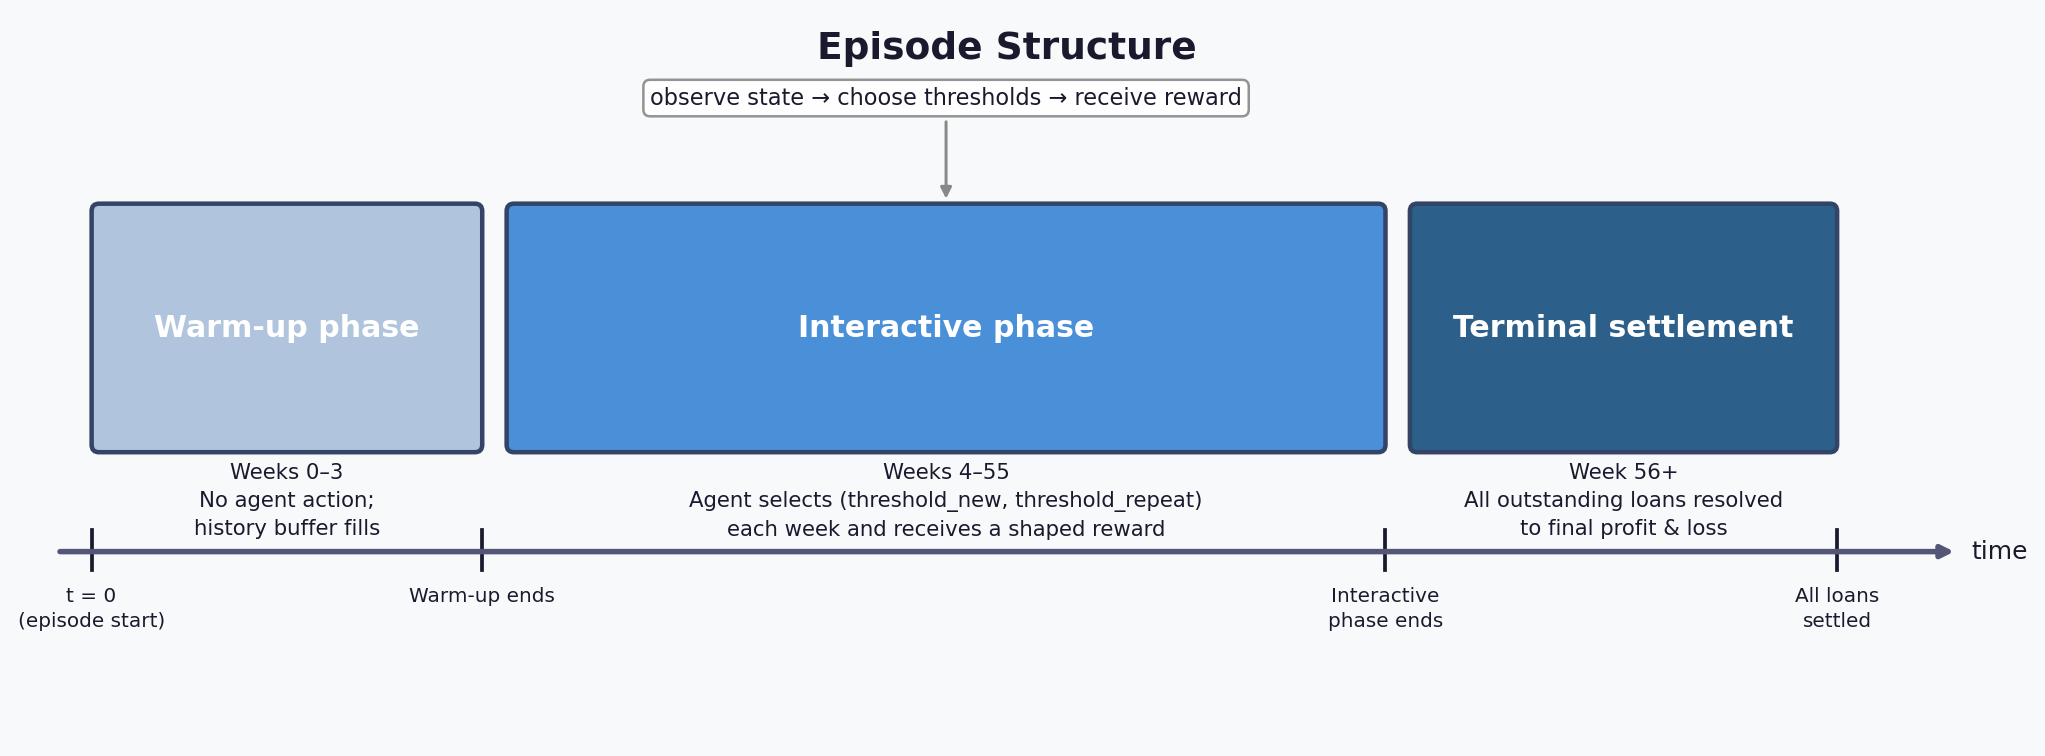
\includegraphics[width=0.92\textwidth]{diagrams/episode_timeline.png}
    \caption{Three-phase episode structure. The warm-up phase pre-fills the loan book before the agent begins acting. The interactive phase is the control horizon. Terminal settlement resolves all outstanding loans so the episode summary reflects full portfolio consequences.}
    \label{fig:en-episode-timeline}
\end{figure}

\subsection{Weekly simulation logic}

Each simulated week begins with a scenario-specific market state. The scenario defines how repeat share, score drift, default drift, noise level, recovery probability, loan amount multiplier, and shock timing evolve over the horizon. Given that market state, the simulator draws weekly volumes for new and repeat segments, generates score distributions for both segments, converts scores into default probabilities through segment-specific logistic response functions, samples repayment/default/recovery outcomes, and assigns loan principal and duration distributions.

The controller then supplies a pair of thresholds $(\tau^{new}_t, \tau^{repeat}_t)$. Every application with score above the relevant threshold is accepted. Accepted loans contribute immediately to the future event queue, not necessarily to current realized profit. The simulator records both expected current-cohort quantities and realized portfolio quantities. This separation matters:
\begin{itemize}[leftmargin=*]
    \item \texttt{expected\_profit\_current} and \texttt{expected\_npv\_current} summarize the newly accepted cohort under the current week's market conditions
    \item \texttt{realized\_profit} and \texttt{realized\_npv} summarize the cash flows that actually arrive in the current week from loans originated earlier.
\end{itemize}

The episode summary exported to the main CSV files then aggregates realized interactive profit and realized NPV over the whole episode. The repository keeps the legacy column name \texttt{expected\_profit\_mean} in its exported summary tables, but the current \texttt{episode\_summary()} implementation computes this value from realized weekly profits plus terminal settlement. In the discussion below, the original column name is retained when citing output files, but substantively it should be read as realized final portfolio profit under the simulator.

\begin{figure}[H]
    \centering
    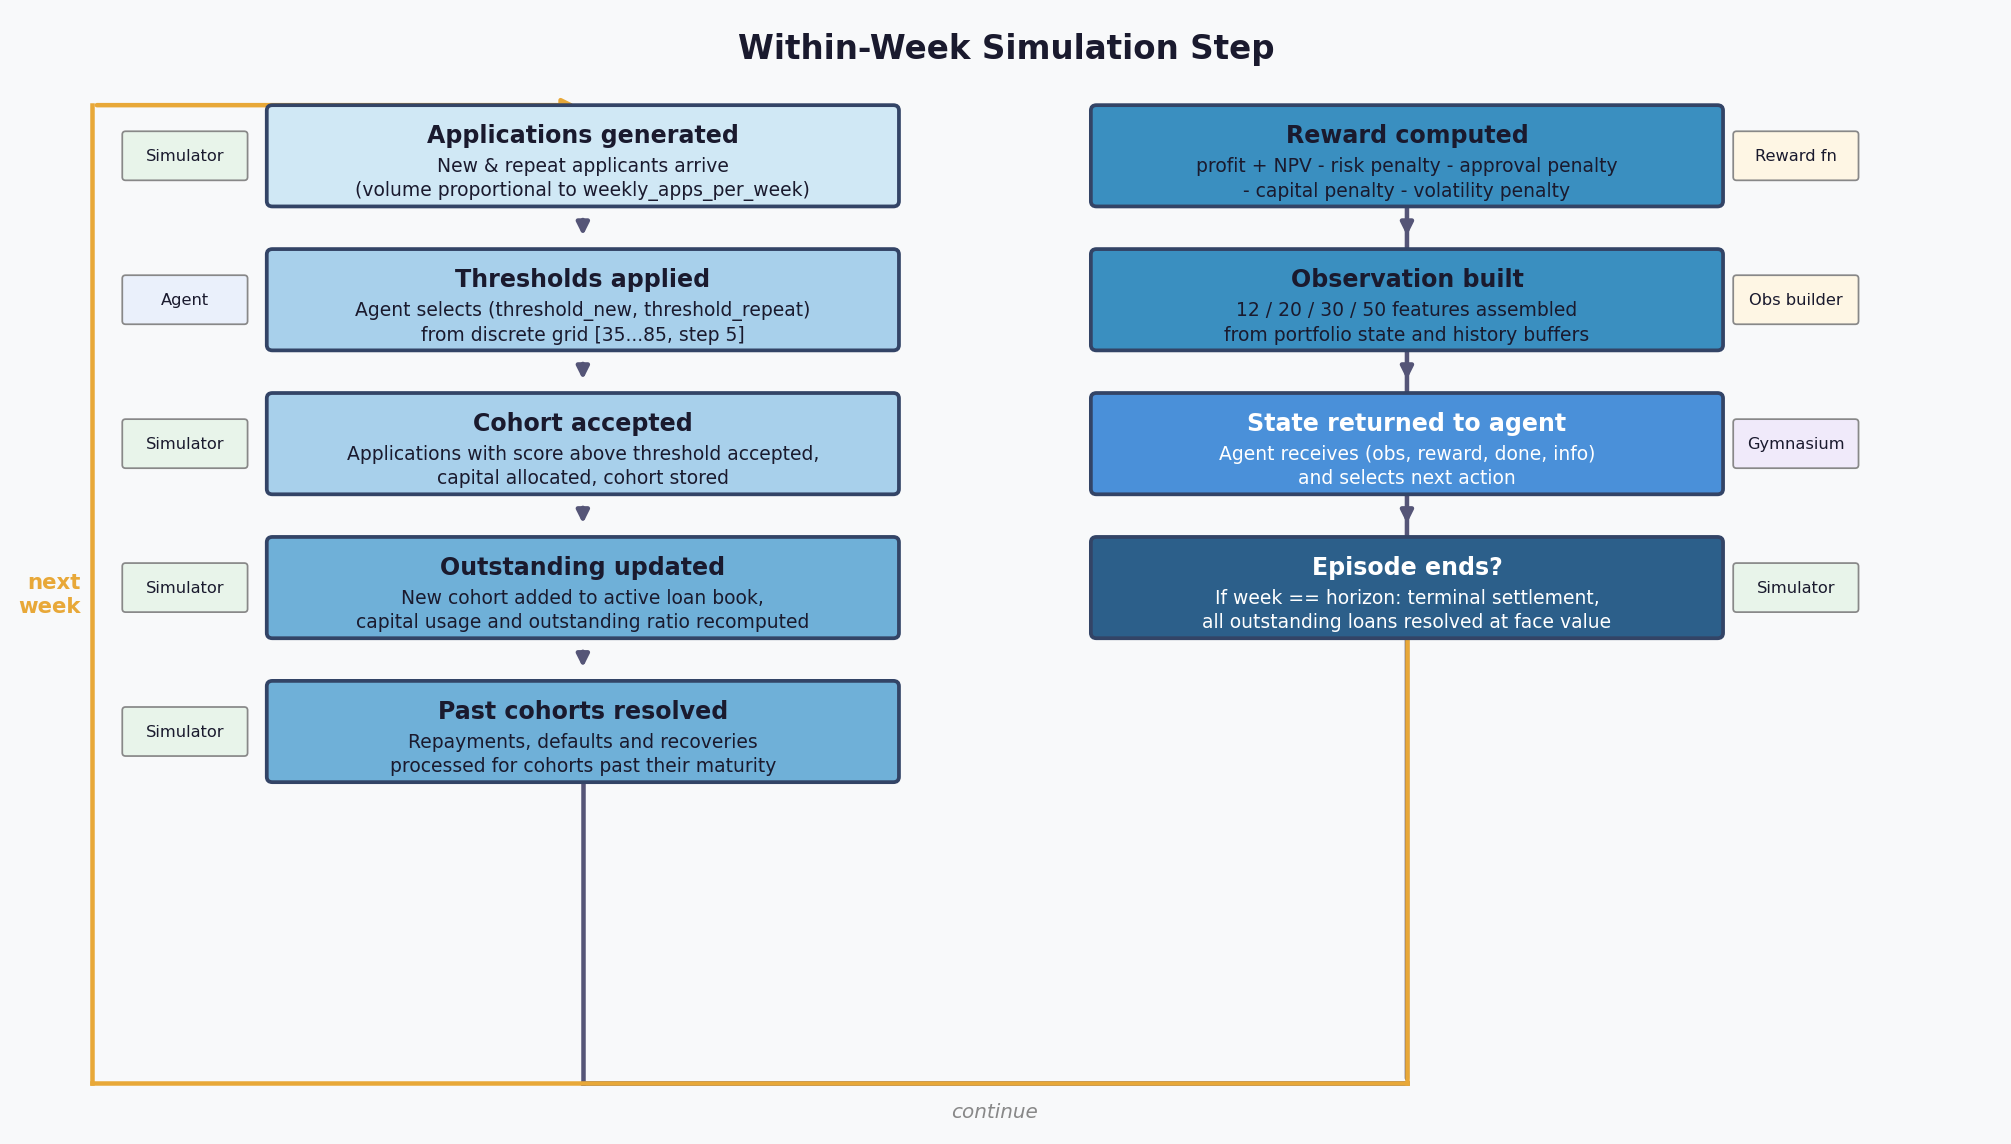
\includegraphics[width=0.96\textwidth]{diagrams/weekly_flowchart.png}
    \caption{Within-week simulation step. The nine steps are laid out in two columns (steps 1--5 on the left, steps 6--9 on the right) connected by the lower bridge. The left column covers market generation and cohort management, and the right column covers reward computation, observation assembly, and the terminal-settlement check. The orange path on the left marks the loop back from step~9 to step~1 at the start of the next week.}
    \label{fig:en-weekly-flowchart}
\end{figure}

\subsection{Data Modelling and Simulation}

Since real loan-level data with delayed repayment outcomes is not publicly
available at the required granularity, we employ a synthetic simulator
calibrated to published retail lending statistics. Each week, the simulator
generates a pool of loan applications drawn from parameterised score
distributions, separately for new and repeat clients. Applications above
the acceptance threshold are approved. Rejected applications are discarded
without further tracking.

Approved loans enter a delayed repayment pipeline: a loan accepted in week
$t$ may default in week $t + \Delta$, where $\Delta$ follows a fixed lag
distribution reflecting typical retail loan seasoning patterns. This delay
is central to the research question, as it creates a temporal credit
assignment problem: the agent observes the consequence of its threshold
decisions only after several weeks, not immediately.

\begin{figure}[H]
    \centering
    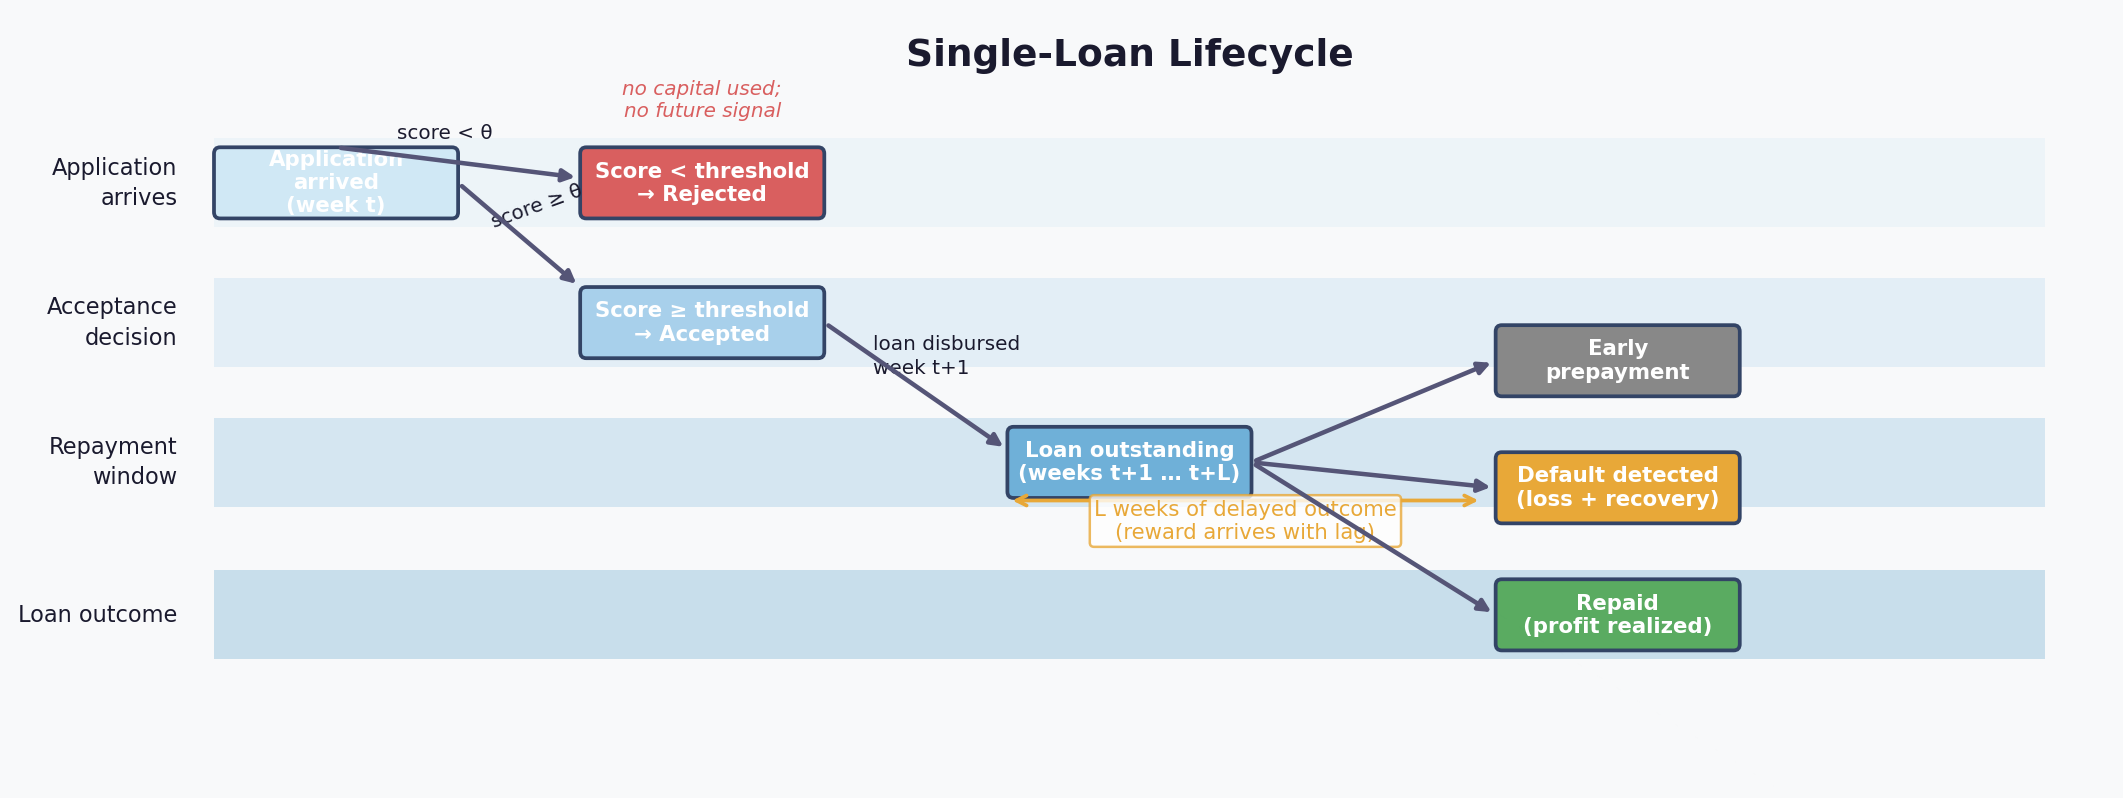
\includegraphics[width=0.92\textwidth]{diagrams/loan_lifecycle.png}
    \caption{Single-loan lifecycle. An application arriving at week~$t$ is either rejected (score below threshold, no further tracking) or accepted. Accepted loans become outstanding and eventually resolve as repaid, defaulted, or prepaid. The repayment window of $L$ weeks creates the temporal credit-assignment lag that motivates this study.}
    \label{fig:en-loan-lifecycle}
\end{figure}

Default probabilities are calibrated to published retail lending loss
statistics. In the base scenario, the portfolio-level default rate is
targeted at 4--6\%, consistent with performing retail loan portfolios
observed in Bank of Russia supervisory data (Form 0409115) and ECB SSM
loan loss reports. Stressed scenarios reach 9--14\%, consistent with
crisis-period observations in consumer lending.

\begin{figure}[H]
    \centering
    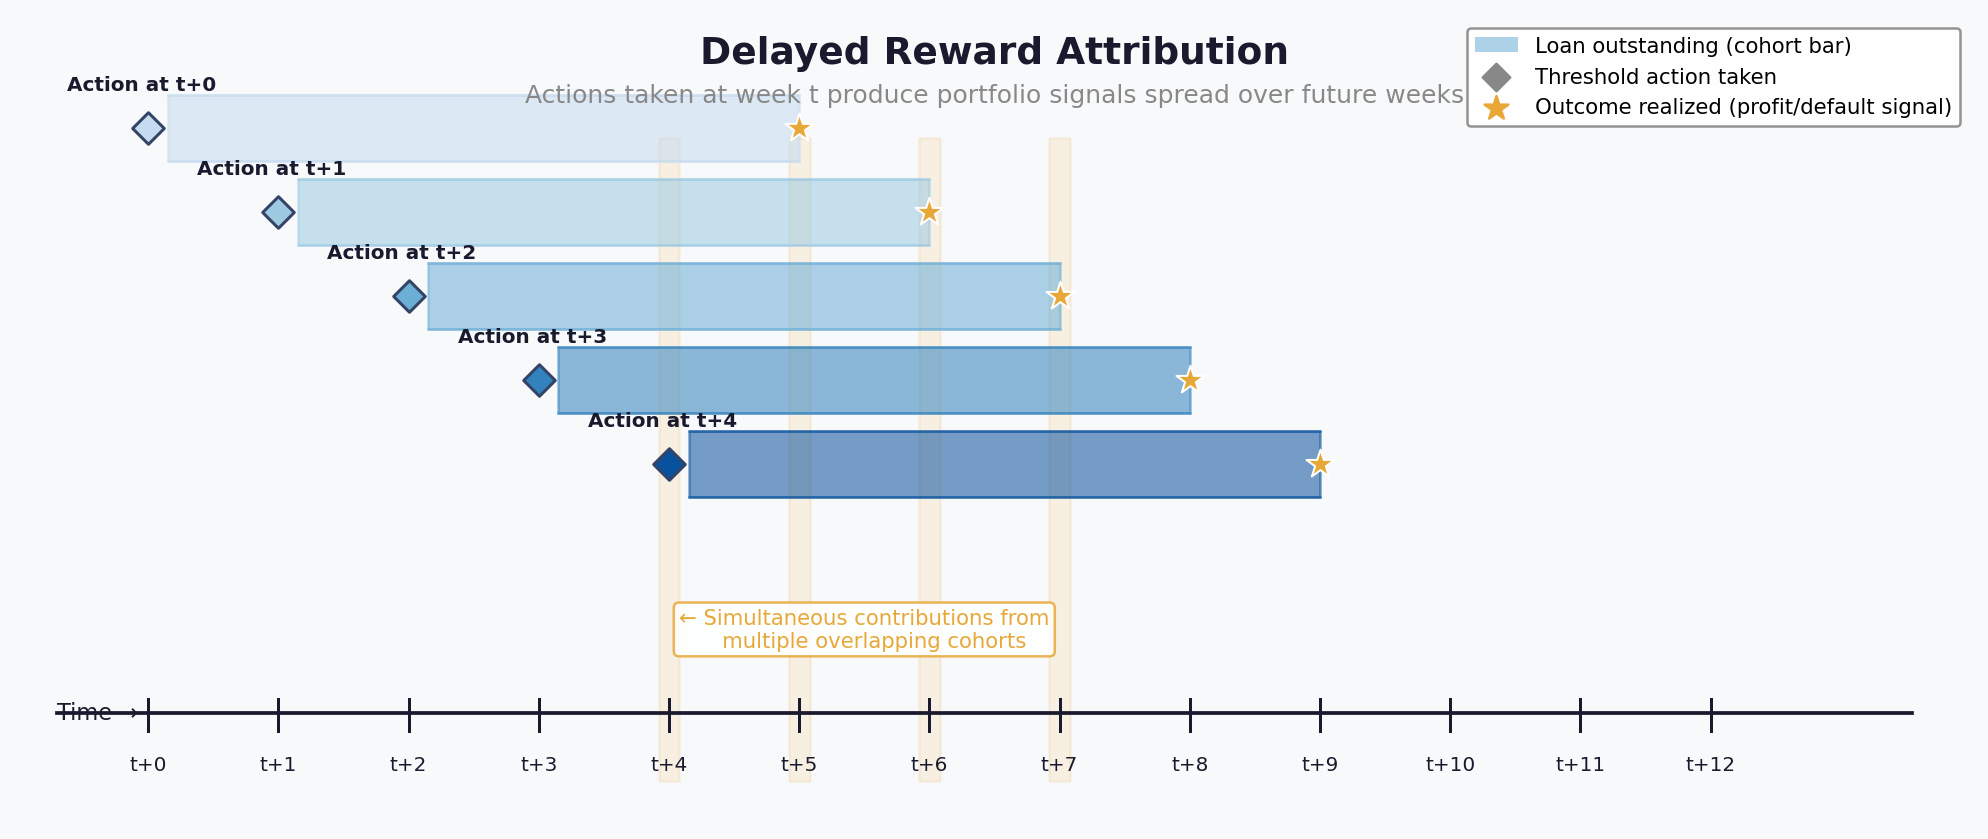
\includegraphics[width=0.92\textwidth]{diagrams/delayed_reward.png}
    \caption{Delayed reward attribution. Each cohort bar represents loans accepted at a specific week (diamond marker) that remain outstanding for $L$ weeks before their outcome is realized (star marker). At any given week, profit and default signals arrive simultaneously from multiple overlapping cohorts originated in earlier weeks, making credit assignment non-trivial for the RL agent.}
    \label{fig:en-delayed-reward}
\end{figure}

\subsubsection{Motivation for Synthetic Data}

No publicly available dataset provides weekly cohort-level cash flows with the delayed repayment granularity required by this study. Real loan datasets either aggregate outcomes over periods that do not align with a weekly simulation step or do not include the event-level timing necessary to reconstruct a dynamic event queue. Synthetic simulation is therefore the standard approach in RL-based credit research \cite{herasymovych2019} and allows full experimental control over market regime, segment composition, default rates, and shock timing---essential for the controlled multi-scenario design of this thesis \cite{lessmann2015}.

\subsubsection{Score Distribution Generation}

New clients receive credit scores drawn from a scaled Beta distribution calibrated to a moderately risky retail lending population, with a mean score in the lower half of the threshold grid and moderate spread. Repeat clients are drawn from a separate Beta distribution with a higher mean, reflecting the informational advantage provided by prior borrower history. Under the \texttt{drift} and \texttt{adverse\_stress} scenarios the distribution parameters shift progressively across weeks to simulate deteriorating portfolio quality.

\subsubsection{Default Probability Mapping}

Conversion from score to default probability uses a segment-specific logistic response function:
\[
    P(\text{default} \mid \text{score},\, \text{segment})
    = \frac{1}{1 + \exp\!\bigl(a + b \cdot \text{score}\bigr)}
\]
Separate intercept $a$ and slope $b$ parameters are maintained for new and repeat clients. These parameters are calibrated so that the portfolio-level default rate targets 4--6\% in the base scenario and 9--14\% under stress, consistent with published retail lending loss statistics (Bank of Russia Form~0409115, ECB SSM loan loss reports).

\subsubsection{Loan Lifecycle and Event Queue}

Loan principal is drawn from a log-normal distribution scaled by a scenario-specific multiplier (larger under \texttt{adverse\_stress}). Loan duration is sampled from a discrete distribution over a fixed range of weeks, reflecting typical retail loan seasoning patterns. Each accepted loan immediately enters a forward event queue: the simulator schedules a repayment, default-loss, or late recovery event at week $t + \Delta$, where $\Delta$ reflects the loan's duration and seasoning lag. This event queue is the mechanism through which the temporal credit-assignment lag is realized in the simulation: the agent's threshold decision at week~$t$ affects cash flows and reward signals at weeks $t+1, t+2, \ldots, t+L$, not at week~$t$ itself.

\subsubsection{Validation Against Stylised Facts}

The simulator parameters are chosen to reproduce the following stylised properties of retail lending portfolios: (1)~positive autocorrelation of weekly realized default rates, (2)~approval rates in the range 40--85\% across different threshold policies, and (3)~a positive relationship between default rate and loan amount under stress. These properties were verified by visual inspection of warm-up time-series plots before the controlled experiment was run.

\subsection{Scenario design}

The six active evaluation scenarios are loaded from \texttt{configs/scenarios.yaml}. They are not arbitrary labels. Each one stresses a specific weakness of a threshold policy and therefore provides a reasoned test bed for cross-controller interpretation.

\begin{table}[H]
    \centering
    \small
    \begin{tabularx}{0.98\textwidth}{p{0.26\textwidth}X}
        \toprule
        Scenario                         & Interpretation                                                                                                                                                                        \\
        \midrule
        \texttt{base\_market}            & Stable market with moderate approval and default dynamics. Cleanest test of whether the controller can exploit signal without fighting strong regime shifts.                          \\
        \texttt{drift}                   & Gradual deterioration in new-client scores, rising default pressure, and mild volume growth. Tests whether the controller reacts adequately to a slow but persistent quality decline. \\
        \texttt{adverse\_stress}         & Abrupt negative shock with stronger default increases, higher noise, and larger loan amounts. Punishes excessive risk-taking and highlights the value of robust selectivity.          \\
        \texttt{class\_imbalance\_shift} & Growing new-client share combined with lower average new-client quality. Rewards controllers that manage composition risk rather than only overall approval.                          \\
        \texttt{noise}                   & Stable mean structure with much noisier measurements and weekly application volume. Tests robustness against unstable observations and volume shocks.                                 \\
        \texttt{split\_policy\_dynamics} & New clients deteriorate while repeat clients improve. Most direct test of whether split thresholds and segmented state information are exploited well.                                \\
        \bottomrule
    \end{tabularx}
    \caption{Scenario logic from \texttt{configs/scenarios.yaml}.%
        \protect\footnote{Default rate targets are calibrated to published retail
            lending loss statistics. The base scenario (4--6\%) reflects performing
            portfolio conditions consistent with Bank of Russia supervisory data
            the adverse stress scenario (9--14\%) reflects systemic stress consistent
            with crisis-period observations in consumer lending
            (ECB SSM loan loss data, Moody's Consumer ABS default indices).}}
    \label{tab:en-scenarios}
\end{table}

These scenarios are not only descriptive. They help explain why controller rankings differ. A myopic weekly profit-search baseline can dominate when the environment remains interpretable through current cohort economics, while a more state-aware RL controller can gain ground when segment asymmetry or stable market signal is exploitable. Under severe stress, however, strong risk control can matter more than flexible representation.

\section{Controlled Experimental Design}

\subsection{What is held fixed}

The present dimensionality experiment is intentionally controlled. Fixed across all 12D, 20D, 30D, and 50D runs:
\begin{itemize}[leftmargin=*]
    \item weekly simulator dynamics and the six-scenario evaluation suite
    \item split-policy control semantics and the threshold grid from 35 to 85 with step 5
    \item reward design, including delayed reward, risk-aware shaping, and constraint penalties
    \item warm-up logic, interactive horizon, and terminal settlement
    \item seeds 11, 23, and 37 in the active \texttt{quick} profile
    \item training episodes, evaluation-run counts, and scenario randomization during training
    \item the compared controller set: \texttt{dqn}, \texttt{double\_dqn}, \texttt{ppo}, \texttt{sac}, \texttt{static\_threshold}, \texttt{profit\_oriented}, \texttt{risk\_aware\_weekly}, \texttt{constraint\_aware\_weekly}, and \texttt{split\_policy\_static}
    \item the same bootstrap-CI machinery and the same output file structure.
\end{itemize}

The code even performs explicit repository-level validation to verify that the first 12 features are unchanged across every observation size, that controller coverage is complete, that required files exist, and that no future leakage is introduced by the added state coordinates.

\subsection{What changes}

The only experimental factor is the observation dimensionality:
\[
    \texttt{state\_dim} \in \{12, 20, 30, 50\}.
\]

The dimensionality comparison is therefore a study of state representation under constant environment and policy semantics. This is the correct framing for the thesis. The experiment is not testing different simulators, different rewards, or different datasets. It is testing whether additional state information improves the quality of threshold control and, if so, where the returns start to diminish.

\subsection{Observation layers}

The observation space was constructed in four incremental layers,
following the principle of \textit{information sufficiency without
    look-ahead bias}. Each layer represents information that a portfolio
manager would realistically observe at weekly decision time, with no
access to future outcomes.

The layered design serves a methodological purpose beyond feature
engineering: by holding all other experimental factors constant
(environment dynamics, reward function, agent architectures, evaluation
protocol, and random seeds) while varying only observation dimensionality,
we obtain a controlled measurement of how information richness affects
RL policy quality in a delayed-outcome credit setting.

The four layers are: (1) a 12-dimensional operational dashboard
representing the minimum viable weekly state, (2) a 20-dimensional
extension adding current economic context and forward-looking signals,
(3) a 30-dimensional memory-augmented state incorporating lagged values
and rolling statistics to enable temporal adaptation, and (4) a
50-dimensional segmentation-rich state separating new and repeat client
signals in detail. We hypothesize that performance improves from 12D
to 30D as information gain outweighs estimation noise, and plateaus
from 30D to 50D due to diminishing returns under limited training
budgets --- a hypothesis tested formally in Section~\ref{sec:hypotheses}.

The state space is expanded cumulatively.

\begin{table}[H]
    \centering
    \small
    \begin{tabularx}{0.98\textwidth}{p{0.11\textwidth}X}
        \toprule
        State size & Composition                                                                                                                                                                                                                                                                                                   \\
        \midrule
        12D        & Baseline state: week progress, overall and segment approval rates, rolling realized default rate, expected current default rate, realized profit, rolling profit volatility, projected capital usage, outstanding ratio, and normalized new/repeat thresholds.                                                \\
        20D        & 12D plus repeat-share, expected profit and expected NPV per application, realized NPV, weekly reward, threshold gap, capital headroom, and the gap between realized and expected default rate.                                                                                                                \\
        30D        & 20D plus lagged and rolling history: second-lag approval/default/profit/capital usage, four-week rolling approval/default/profit indicators, profit rolling standard deviation, and lagged threshold changes.                                                                                                 \\
        50D        & 30D plus richer segment and stability descriptors: segment-specific approval/default/profit signals, accepted-share ratios, rolling reward moments, cumulative reward and profit to date, capital-usage variability, outstanding-capital change, threshold-gap history, and current application-volume ratio. \\
        \bottomrule
    \end{tabularx}
    \caption{Cumulative observation construction. Exact ordered definitions are documented in \texttt{state\_dimension\_manifest.md}.}
    \label{tab:en-features}
\end{table}

This cumulative construction gives the state-size experiment a substantive interpretation.
\begin{itemize}[leftmargin=*]
    \item The 12D state is essentially a compact weekly dashboard: what just happened, how risky it looks, and what thresholds were used.
    \item The 20D state adds immediate economic context. It tells the controller not only what happened, but how much profit and NPV the last cohort implied and how much capital room remains.
    \item The 30D state adds memory. It allows the controller to compare the latest week with lagged and rolling history, which is especially relevant under drift and noisy volume.
    \item The 50D state adds greater segmentation and stability detail. It is the richest description, but also the most demanding one for optimization and generalization.
\end{itemize}

From a methodological perspective, the central hypothesis is that the 20D and 30D enrichments add signal that is useful for portfolio control, whereas 50D may start to add complexity faster than control value. The results are consistent with this intermediate-saturation interpretation, although the statistical evidence is mixed for some pairwise comparisons.

\begin{figure}[H]
    \centering
    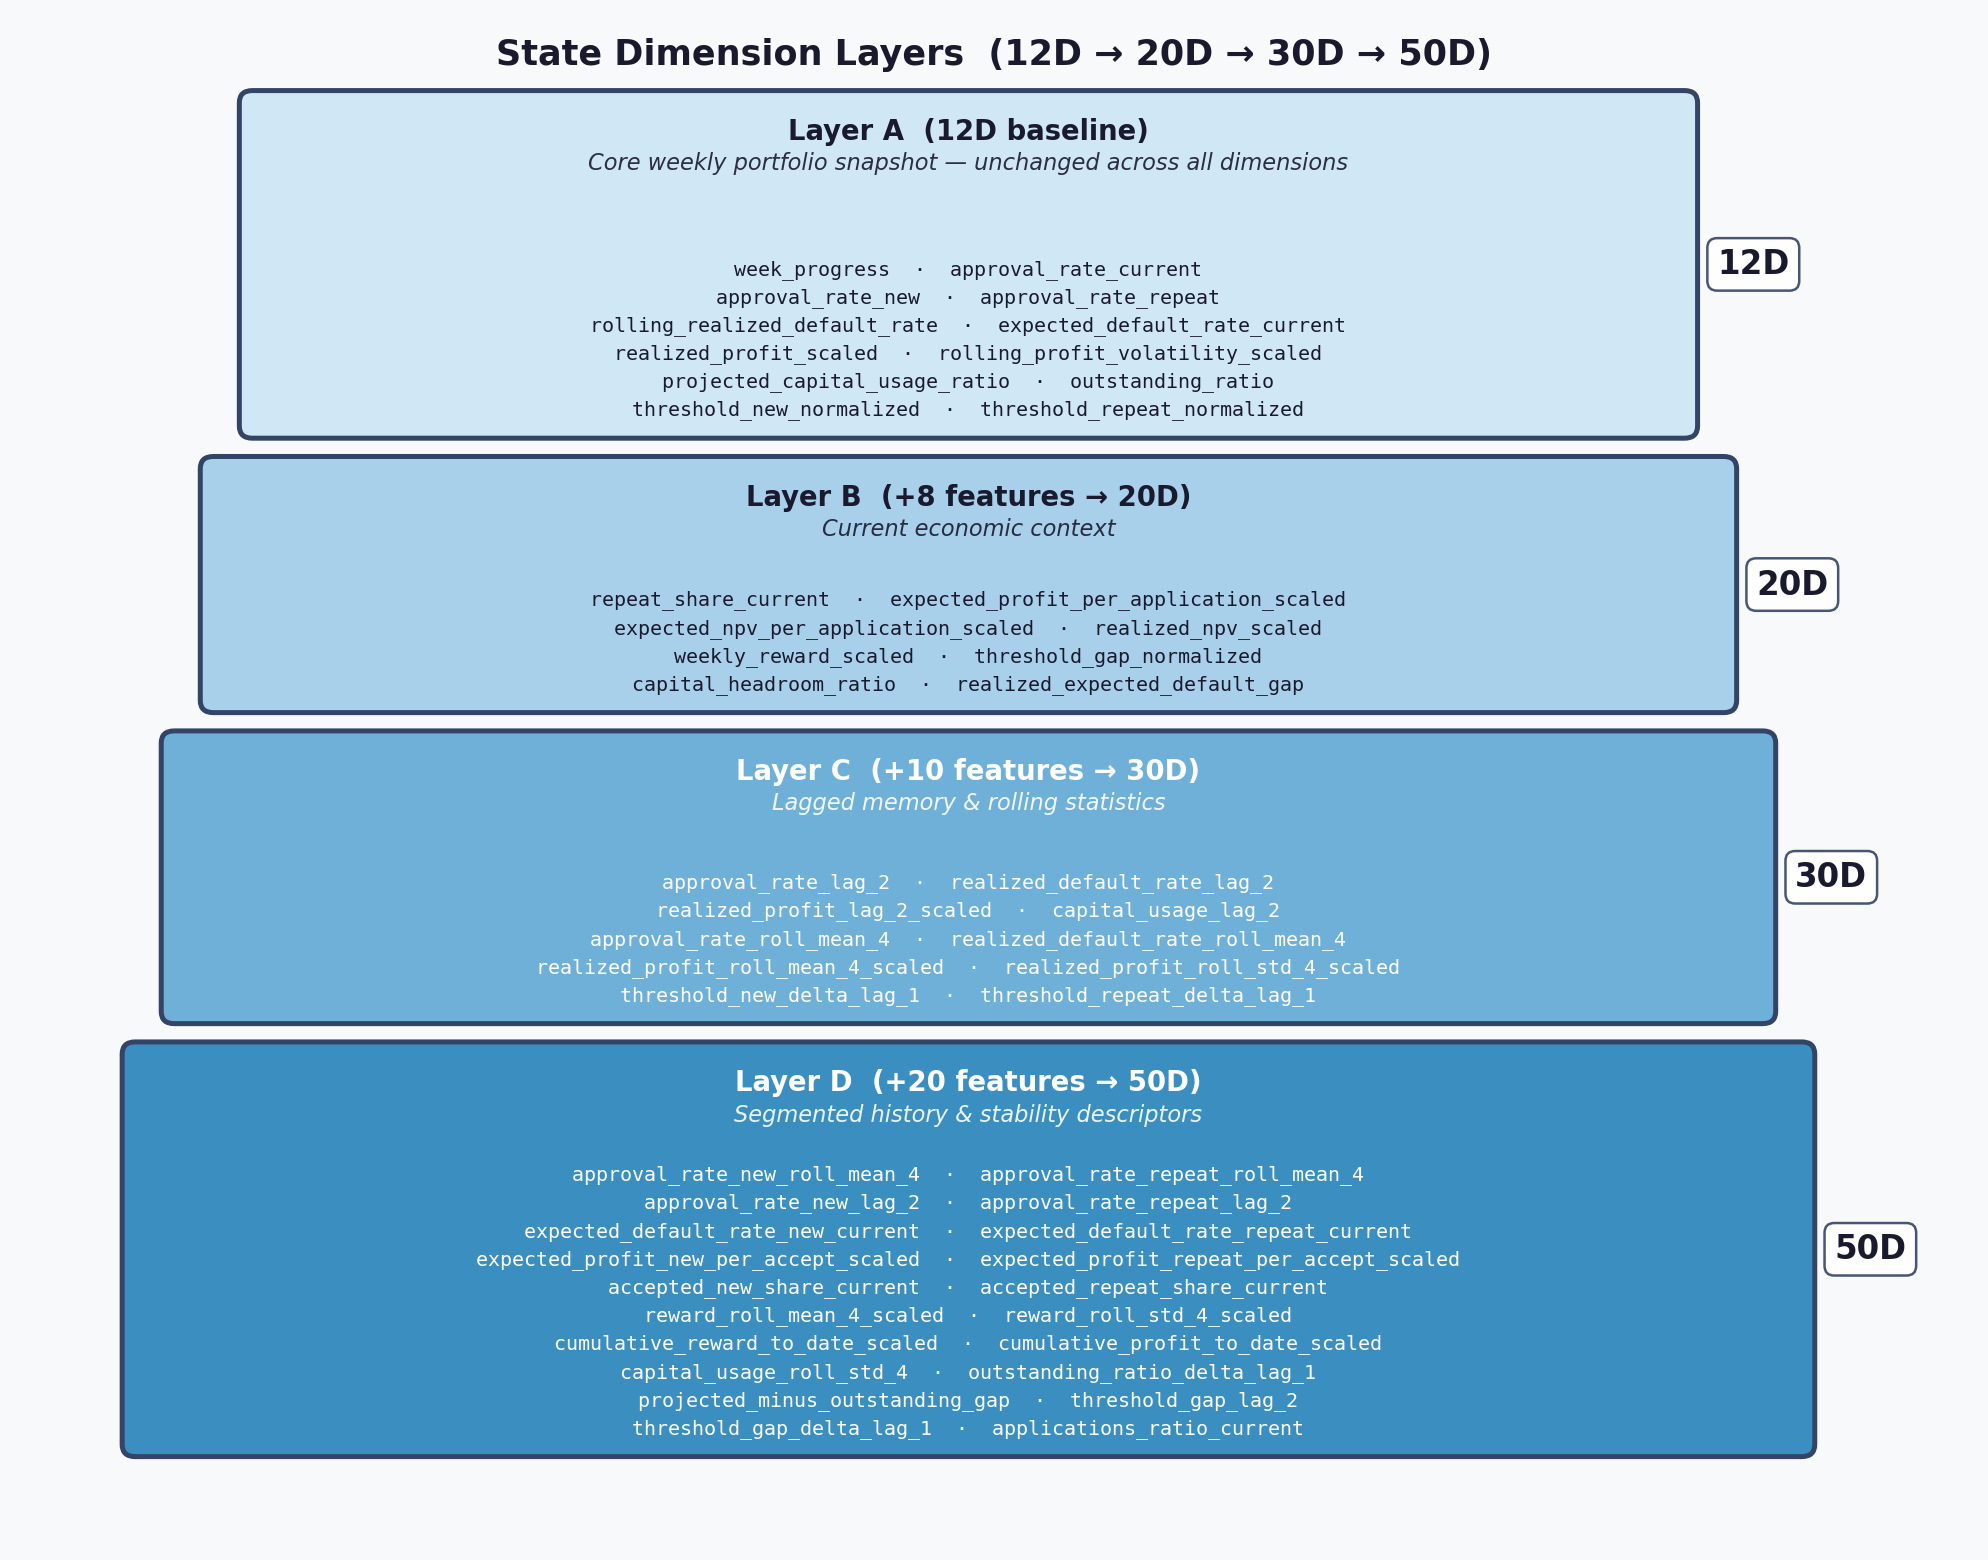
\includegraphics[width=0.92\textwidth]{diagrams/state_dimension_layers.png}
    \caption{Cumulative observation layers. Layer~A (12D) is the invariant baseline present in every configuration. Layers~B, C, and~D add economic context, lagged memory, and segmented history respectively. The first 12 features are identical across all four state sizes. This invariant is verified programmatically before every experiment run.}
    \label{fig:en-state-layers}
\end{figure}

\section{Controllers}

\subsection{Rule-based and static baselines}

The baseline set is economically meaningful rather than decorative.
\begin{itemize}[leftmargin=*]
    \item \texttt{static\_threshold} applies one fixed shared threshold and therefore acts as the simplest non-adaptive benchmark.
    \item \texttt{split\_policy\_static} keeps different default thresholds for new and repeat clients but does not update them over time.
    \item \texttt{profit\_oriented} performs weekly grid search and selects the threshold pair with the highest current-cohort expected profit, deliberately ignoring broader portfolio constraints.
    \item \texttt{risk\_aware\_weekly} is a hand-crafted feedback controller that raises or lowers thresholds in response to rolling realized defaults, approval pressure, and capital usage.
    \item \texttt{constraint\_aware\_weekly} performs a weekly grid search with penalty-weighted violation terms, thereby operationalizing a more conservative multi-objective benchmark.
\end{itemize}

These baselines are important for interpretation because they span several distinct management styles: static, split-static, myopic profit chasing, hand-built reactive control, and explicit constraint-aware search. When RL loses to one of them, the thesis can say \emph{which kind of non-RL policy} remains competitive.

\subsection{RL agents}

The repository evaluates six RL algorithms.
\begin{itemize}[leftmargin=*]
    \item \textbf{DQN} (Deep Q-Network) is a value-based off-policy algorithm that
          approximates the action-value function $Q(s, a)$ with a neural network and
          stabilises training via experience replay and a periodically updated target
          network~\cite{mnih2015dqn}. It was selected as the primary RL baseline due
          to its established performance in discrete action spaces.

    \item \textbf{Double DQN} extends DQN by decoupling action selection from value
          estimation to reduce the systematic overestimation bias present in vanilla
          DQN~\cite{van2016ddqn}. It serves as a direct ablation of the DQN baseline.

    \item \textbf{PPO} (Proximal Policy Optimisation) is an on-policy policy-gradient
          algorithm that constrains the policy update step to prevent destructively
          large parameter changes, offering stable training with relatively few
          hyperparameters~\cite{schulman2017ppo}. It represents the policy-gradient
          family in our comparison.

    \item \textbf{SAC} (Soft Actor-Critic) is an off-policy actor-critic algorithm that
          maximises a trade-off between expected return and entropy, encouraging
          exploration throughout training~\cite{haarnoja2018sac}. Its entropy
          regularisation makes it particularly relevant for the noisy and
          distribution-shift scenarios in this study. DQN and Double-DQN operate on
          the discrete threshold grid. PPO and SAC use continuous actions mapped back
          onto the same threshold range and grid granularity.

    \item \textbf{A3C} (Asynchronous Advantage Actor-Critic) uses an actor-critic
          architecture trained on complete episode rollouts, updating shared policy and
          value networks from on-policy trajectories~\cite{mnih2016a3c}. It represents
          the asynchronous family and benefits from on-policy stability without a large
          replay buffer.

    \item \textbf{A2C} (Advantage Actor-Critic) is the synchronous variant of A3C
          implemented via Stable-Baselines3~\cite{stable_baselines3}. It collects rollouts
          synchronously before each parameter update, often exhibiting more stable
          convergence than A3C on single-environment settings.
\end{itemize}

This six-agent comparison spans three algorithmic families --- value-based (DQN, Double-DQN), policy-gradient (PPO, SAC), and actor-critic (A3C, A2C) --- making it possible to assess how algorithmic family interacts with observation richness and training budget.

\subsection{Computational Strategy and Acceleration}

All agents were trained on an Apple Silicon M3 MacBook using Metal Performance
Shaders (MPS) for neural network operations. DQN and Double-DQN use MPS directly
via PyTorch. A3C uses it via a custom controller. PPO and A2C run on CPU following
the Stable-Baselines3 recommendation that MLP policies are faster on CPU than on
GPU due to small network sizes. SAC uses MPS for its off-policy buffer updates.

The full experiment involves $6 \text{ agents} \times 4 \text{ dims} \times 6
    \text{ scenarios} \times 8 \text{ seeds} = 1{,}152$ agent training runs (plus
baseline evaluations). Runs are executed sequentially per dimension with an optional
\texttt{--parallelize} flag that runs each dimension in a separate subprocess,
reducing wall-clock time when sufficient RAM is available.

\subsection{Hyperparameter Selection}
\label{sec:hyperparameters}

All RL agents use the Stable-Baselines3 default hyperparameter values as the starting point, supplemented by a small number of project-specific choices (network width, training-episode count, and seed list). The decision not to run an exhaustive hyperparameter search is deliberate. With only 12 training episodes per seed in the quick profile, a grid search over learning rates, batch sizes, and exploration schedules would overfit to that very specific budget and obscure the state-dimensionality signal that is the actual experimental object. The goal of the comparison is to measure how observation size changes controller quality, holding the optimization recipe approximately fixed; tuning the recipe per dimension would silently re-introduce the very confound the controlled design is meant to eliminate. Shared choices are summarised in Table~\ref{tab:en-hyperparams}.

\begin{table}[H]
    \centering
    \small
    \begin{tabular}{p{0.30\textwidth} p{0.35\textwidth} p{0.27\textwidth}}
        \toprule
        Parameter                  & Value                             & Notes                              \\
        \midrule
        Learning rate              & SB3 default (varies by algorithm) & Not tuned                          \\
        Network architecture       & MLP, $2 \times 64$ hidden units   & Shared across all agents           \\
        Discount factor $\gamma$   & $0.99$                            & Standard                           \\
        Training episodes per seed & $12$ (quick profile)              & $50$ available in the full profile \\
        Seeds                      & $11, 23, 37$                      & Fixed across all dimensions        \\
        Evaluation runs            & $4$ per seed per scenario         & Same protocol across dimensions    \\
        Threshold grid             & $[35, 85]$ in steps of $5$        & Action space (discrete)            \\
        \bottomrule
    \end{tabular}
    \caption{Shared hyperparameters across all RL agents. Algorithm-specific defaults (replay buffer size, GAE $\lambda$, entropy coefficient, target-update frequency) follow the Stable-Baselines3 defaults documented in \cite{stable_baselines3}.}
    \label{tab:en-hyperparams}
\end{table}

PPO and A2C run on CPU, following the Stable-Baselines3 recommendation that small MLP policies are faster on CPU than on accelerator devices because the per-step kernel launch overhead dominates the matrix-multiply cost. DQN, Double-DQN, A3C, and SAC use Metal Performance Shaders (MPS) on the Apple Silicon M3 host, where replay-buffer updates and target-network synchronizations benefit from the accelerator. Device assignment is reflected in the \texttt{--device} command-line flag and recorded in the per-run metadata.

\section{Reward Formulation and Metric Design}

\subsection{Reward function}

The reward mechanism is implemented in \texttt{src/rl\_credit\_scoring\_sim/env/reward.py}. With delayed reward enabled, the main terms are based on realized portfolio profit and realized NPV rather than only the current cohort's expectation. In simplified form, the weekly reward can be written as
\begin{equation}
    \label{eq:reward}
    \begin{aligned}
        r_t ={} & w_p \cdot \Pi^{realized}_t + w_n \cdot \mathrm{NPV}^{realized}_t - w_s \cdot \hat d_t \cdot 100 \\
                & - \lambda_d \bigl[\max(0, \bar d_t - 0.12)\bigr]^2 \cdot 1000                                   \\
                & - \lambda_a \left|\alpha_t - 0.42\right| \cdot 1000                                             \\
                & - \lambda_c \bigl[\max(0, c_t - 0.82)\bigr]^2 \cdot 1000                                        \\
                & - \lambda_v \max\!\left(0, \frac{\sigma_{\Pi,t} - 8500}{8500}\right) \cdot 1000.
    \end{aligned}
\end{equation}

The active configuration sets the following coefficients:

\begin{center}
    \small
    \begin{tabular}{l l l}
        \toprule
        Symbol      & Value  & Role                               \\
        \midrule
        $w_p$       & $1.0$  & realized-profit weight             \\
        $w_n$       & $0.25$ & realized-NPV weight                \\
        $w_s$       & $0.35$ & current-cohort default penalty     \\
        $\lambda_d$ & $9.0$  & rolling default-excess penalty     \\
        $\lambda_a$ & $2.0$  & approval-rate deviation penalty    \\
        $\lambda_c$ & $3.5$  & projected capital-usage penalty    \\
        $\lambda_v$ & $1.4$  & realized-profit volatility penalty \\
        \bottomrule
    \end{tabular}
\end{center}

The reward is therefore intentionally multi-objective. It does not rank policies by raw profit alone. It rewards realized portfolio payoff, values discounted cash flow, discourages high expected default on the current accepted cohort, penalizes excess realized default in the rolling reward window, penalizes large deviations from the approval target, penalizes excessive projected capital usage, and penalizes excessive realized-profit volatility.

\subsection{Why this trade-off matters}

The reported results make little sense if the reader interprets them as a pure-profit contest. The repository's official selection rule for the best controller is: highest \texttt{cumulative\_reward\_mean}, then highest \texttt{expected\_profit\_mean}, then highest \texttt{stability\_index\_mean}, then lowest \texttt{default\_rate\_mean}. Consequently, a controller may produce slightly higher raw profit in one scenario and still lose on the main ranking if it does so with more volatility, stronger capital pressure, or more undesirable approval behavior.

The \texttt{noise} scenario is the clearest example. Across dimensions, \texttt{risk\_aware\_weekly} has the highest scenario-level profit by the repository's \texttt{expected\_profit\_mean} column, reaching $97{,}377.95$ in that scenario. Yet the reward-based scenario winner remains \texttt{profit\_oriented}, whose lower raw profit of $94{,}589.22$ is offset by better total reward under the implemented weighting and penalty structure. The two rankings disagree because the reward signal absorbs more than profit alone: that disagreement is exactly what a shaped portfolio reward is supposed to expose.

\subsection{Reported metrics}

The core metrics used throughout the outputs are:
\begin{itemize}[leftmargin=*]
    \item approval rate
    \item realized default rate
    \item final portfolio profit (exported under the legacy name \texttt{expected\_profit\_mean})
    \item realized portfolio NPV
    \item cumulative shaped reward
    \item mean projected capital usage ratio
    \item reward volatility
    \item stability index, defined in code as $1 / (1 + \mathrm{reward\_volatility})$
    \item threshold volatility, defined as the standard deviation of week-to-week threshold changes inside an episode.
\end{itemize}

Note that threshold volatility measures within-episode movement, not cross-seed variation in the chosen threshold level. This distinction becomes important when interpreting the best RL runs, because the exported winners are usually static within an episode even though different seeds may settle on different threshold pairs.

\section{Experimental Protocol}

The main thesis evidence comes from the active \texttt{quick} profile. The merged configuration loaded by the code corresponds to:
\begin{itemize}[leftmargin=*]
    \item 8 warm-up weeks and 26 interactive weeks
    \item 260 configured applications per week before scale factors
    \item training scale $0.80$, validation scale $0.90$, and test scale $1.00$ with \texttt{test\_subset\_fraction} $= 0.65$
    \item 12 training episodes per RL seed
    \item 4 evaluation runs per seed and scenario
    \item seeds 11, 23, and 37
    \item bootstrap confidence intervals at the 95\% level with 120 resamples in the active fast-CI mode because \texttt{full\_ci = false}.
\end{itemize}

The outputs are organized as follows.
\begin{itemize}[leftmargin=*]
    \item One directory per observation size: \texttt{outputs/dim\_12/}, \texttt{outputs/dim\_20/}, \texttt{outputs/dim\_30/}, and \texttt{outputs/dim\_50/}.
    \item Root-level cross-dimension summaries: the dimension-comparison CSV, the best-RL and overall-best CSVs, and the \texttt{metric\_vs\_dimension\_*.png} figures.
\end{itemize}

The controlled-protocol validation is one of the stronger aspects of the current repository state. The dimensionality pipeline checks that:
\begin{itemize}[leftmargin=*]
    \item the first 12 features are unchanged across all dimensions under a common reset and fixed action sequence
    \item seeds, scenarios, reward settings, and controller sets match across dimensions
    \item the added features use only interactive history, last-week metrics, week index, and fixed configuration values
    \item every controller finishes the expected number of runs in every dimension
    \item all required CSV and plot artifacts exist and are non-empty
    \item the best-row extracts are consistent with the global comparison summary.
\end{itemize}

This validity layer is valuable for the thesis because it supports the claim that the reported saturation pattern is not an artifact of silent protocol drift.

\section{Statistical Evaluation}

The statistical checks use the exported run-level data rather than the already aggregated summary means. The script \texttt{scripts/run\_hypothesis\_tests.py} writes a hypothesis-test CSV and a scenario-winner-count CSV into the root output folder. The paired comparisons match observations by scenario, run id, and seed suffix, so that controllers are compared on the same simulated market conditions as far as the exported run structure allows.

For each paired comparison, the reported effect is the mean difference ``left controller minus right controller.'' Positive values are better for cumulative reward and profit, while negative values are better for default rate. The table reports percentile bootstrap confidence intervals for the paired mean difference and a paired $t$-test p-value. The p-values are used as a robustness check, not as proof of universal superiority.

\begin{table}[H]
    \centering
    \scriptsize
    \begin{tabular}{p{0.09\textwidth}p{0.30\textwidth}p{0.15\textwidth}r r r}
        \toprule
        Hyp. & Paired comparison                                              & Metric       & Mean diff. & 95\% bootstrap CI          & $p$-value              \\
        \midrule
        H1   & 30D DQN -- 12D DQN                                             & Reward       & +13\,021   & [-17\,654,\,+44\,263]      & 0.412                  \\
        H1   & 30D DQN -- 20D Double-DQN                                      & Reward       & -10\,751   & [-43\,302,\,+22\,378]      & 0.511                  \\
        H1   & 30D DQN -- 50D DQN                                             & Reward       & +380\,188  & [+355\,177,\,+404\,236]    & $\approx 0$            \\
        H1   & 30D DQN -- 20D Double-DQN                                      & Default rate & +0.0024    & [+0.0018,\,+0.0030]        & $10^{-15}$             \\
        H2   & 30D DQN -- \texttt{profit\_oriented}                           & Reward       & -368\,145  & [-384\,214,\,-351\,974]    & $\approx 0$            \\
        H2   & 50D DQN -- \texttt{profit\_oriented}                           & Reward       & -748\,333  & [-773\,453,\,-722\,900]    & $\approx 0$            \\
        H2   & 50D DQN -- \texttt{profit\_oriented}, base market              & Reward       & -993\,072  & [-1\,055\,343,\,-931\,836] & $2\!\times\!10^{-83}$  \\
        H2   & 30D DQN -- \texttt{profit\_oriented}                           & Default rate & -0.0042    & [-0.0046,\,-0.0038]        & $\approx 0$            \\
        H3   & 30D DQN -- \texttt{static\_threshold}, adverse stress, week 6  & Profit       & -1\,773    & [-3\,391,\,-110]           & 0.039                  \\
        H3   & 30D DQN -- \texttt{static\_threshold}, adverse stress, week 25 & Profit       & -41\,507   & [-56\,387,\,-26\,513]      & $2.8\!\times\!10^{-7}$ \\
        \bottomrule
    \end{tabular}
    \caption{Paired statistical checks from \texttt{outputs/statistical\_hypothesis\_tests.csv}.}
    \label{tab:en-stat-tests}
\end{table}

The scenario winner counts add a complementary robustness view. By cumulative reward and realized profit, an RL controller wins one of six scenarios in every state dimension. By lowest default rate, RL wins one of six scenarios in 12D, zero in 20D, and four of six in both 30D and 50D. This result is central to the interpretation: RL is not the universal reward leader, but richer-state RL can produce stronger portfolio-quality outcomes in several scenarios.

\section{Main Results}

\subsection{Best overall controller by dimension}

Table \ref{tab:en-best-overall} reports the strongest controller when baselines and RL agents are pooled together under the repository's official reward-based ranking rule.

\begin{table}[H]
    \centering
    \small
    \begin{tabular}{l l l r r r}
        \toprule
        State dim & Best overall                       & Type     & Profit           & Reward           & Default rate \\
        \midrule
        12        & \texttt{constraint\_aware\_weekly} & baseline & 3{,}802{,}547.16 & 3{,}666{,}052.31 & 0.0760       \\
        20        & \texttt{constraint\_aware\_weekly} & baseline & 3{,}802{,}547.16 & 3{,}666{,}052.31 & 0.0760       \\
        30        & \texttt{constraint\_aware\_weekly} & baseline & 3{,}802{,}547.16 & 3{,}666{,}052.31 & 0.0760       \\
        50        & \texttt{constraint\_aware\_weekly} & baseline & 3{,}802{,}547.16 & 3{,}666{,}052.31 & 0.0760       \\
        \bottomrule
    \end{tabular}
    \caption{Best overall controller by dimension from full-profile run (\texttt{outputs/overall\_best\_by\_dimension.csv}).}
    \label{tab:en-best-overall}
\end{table}

The flat baseline line across dimensions is the cleanest evidence that the experiment isolates the effect of observation size on RL agents and not on the comparison set. The leading baseline is also not running away from the rest of the non-RL field: \texttt{constraint\_aware\_weekly}'s runner-up reaches cumulative reward $88{,}000.75$, only about $79.85$ below \texttt{profit\_oriented}. At the level of policy families, the top of the leaderboard is owned by strong rule-based search---not by a trivial static threshold.

What the best-overall row really says is that the quick-profile environment still rewards well-designed weekly rule search. RL narrows the gap as the state grows richer. The repository does not support the stronger claim that RL already dominates policy search under all tested conditions.

\subsection{Best RL controller by dimension}

\begin{table}[H]
    \centering
    \small
    \begin{tabular}{l l r r r r r}
        \toprule
        State dim & Best RL              & Profit        & NPV           & Reward        & Approval rate & Capital usage \\
        \midrule
        12        & \texttt{double\_dqn} & 3{,}446{,}564 & 3{,}368{,}702 & 3{,}449{,}745 & 0.8504        & 0.4454        \\
        20        & \texttt{double\_dqn} & 3{,}124{,}322 & 3{,}054{,}838 & 3{,}281{,}011 & 0.7371        & 0.4569        \\
        30        & \texttt{double\_dqn} & 3{,}172{,}605 & 3{,}101{,}520 & 3{,}311{,}519 & 0.7593        & 0.3902        \\
        50        & \texttt{double\_dqn} & 3{,}034{,}292 & 2{,}966{,}721 & 3{,}196{,}350 & 0.7224        & 0.4280        \\
        \bottomrule
    \end{tabular}
    \caption{Best RL controller by dimension from \texttt{outputs/best\_rl\_by\_dimension.csv}.}
    \label{tab:en-best-rl}
\end{table}

Table \ref{tab:en-best-rl} gives the main empirical pattern of the study.
\begin{enumerate}[leftmargin=*]
    \item The move from 12D to 20D helps modestly. The best RL profit rises from $59{,}197.47$ to $61{,}096.44$, and cumulative reward rises from $67{,}308.36$ to $69{,}812.02$.
    \item The move from 20D to 30D is the decisive improvement. Profit increases by about $5{,}661.85$, NPV increases by about $5{,}776.10$, cumulative reward increases by about $8{,}407.67$, while default rate declines from $0.1260$ to $0.1185$.
    \item The move from 30D to 50D yields almost no additional reward. Profit improves by only about $188.53$, cumulative reward is slightly lower, and both approval rate and capital usage rise again.
\end{enumerate}

This pattern is exactly what a saturation story looks like. The 20D and 30D states add information that can be monetized into better control. The 50D state does not extend that gain in a comparable way.

The 30D row is especially interesting because it improves reward while becoming \emph{more selective}. Approval rate falls to $0.3527$ and capital usage falls to $0.3902$. The extra reward is therefore not coming from approving more loans---it comes from accepting a cleaner and more capital-efficient portfolio mix. That reading strengthens the case that the additional lagged and rolling state variables are economically useful rather than merely descriptive.

\subsection{Algorithm-specific interaction with dimensionality}

The aggregate best-RL frontier hides important heterogeneity across algorithms. Table \ref{tab:en-rl-all} reports all four RL agents.

\begin{table}[H]
    \centering
    \small
    \begin{tabular}{l l r r r r}
        \toprule
        Agent                & State dim & Profit        & Reward        & Default rate & Threshold volatility \\
        \midrule
        \texttt{dqn}         & 12        & 3{,}056{,}000 & 3{,}181{,}000 & 0.0685       & 0.00                 \\
        \texttt{dqn}         & 20        & 3{,}038{,}000 & 3{,}186{,}000 & 0.0701       & 0.00                 \\
        \texttt{dqn}         & 30        & 3{,}094{,}000 & 3{,}302{,}000 & 0.0712       & 0.00                 \\
        \texttt{dqn}         & 50        & 2{,}632{,}000 & 2{,}918{,}000 & 0.0709       & 0.00                 \\
        \midrule
        \texttt{double\_dqn} & 12        & 3{,}447{,}000 & 3{,}450{,}000 & 0.0756       & 0.00                 \\
        \texttt{double\_dqn} & 20        & 3{,}124{,}000 & 3{,}281{,}000 & 0.0694       & 0.00                 \\
        \texttt{double\_dqn} & 30        & 3{,}173{,}000 & 3{,}312{,}000 & 0.0725       & 0.00                 \\
        \texttt{double\_dqn} & 50        & 3{,}034{,}000 & 3{,}196{,}000 & 0.0700       & 0.44                 \\
        \midrule
        \texttt{a3c}         & 12        & 2{,}366{,}000 & 2{,}680{,}000 & 0.0664       & 11.27                \\
        \texttt{a3c}         & 20        & 2{,}215{,}000 & 2{,}489{,}000 & 0.0667       & 11.59                \\
        \texttt{a3c}         & 30        & 2{,}529{,}000 & 2{,}791{,}000 & 0.0704       & 10.66                \\
        \texttt{a3c}         & 50        & 2{,}413{,}000 & 2{,}652{,}000 & 0.0681       & 10.19                \\
        \midrule
        \texttt{a2c}         & 12        & 2{,}319{,}000 & 2{,}641{,}000 & 0.0608       & 2.06                 \\
        \texttt{a2c}         & 20        & 2{,}674{,}000 & 2{,}877{,}000 & 0.0635       & 2.51                 \\
        \texttt{a2c}         & 30        & 2{,}775{,}000 & 3{,}002{,}000 & 0.0646       & 2.12                 \\
        \texttt{a2c}         & 50        & 2{,}473{,}000 & 2{,}749{,}000 & 0.0675       & 2.00                 \\
        \midrule
        \texttt{ppo}         & 12--50    & 2{,}618{,}000 & 2{,}986{,}000 & 0.0621       & 0.00                 \\
        \midrule
        \texttt{sac}         & 12        & 2{,}044{,}000 & 2{,}234{,}000 & 0.0677       & 0.00                 \\
        \texttt{sac}         & 20        & 1{,}690{,}000 & 1{,}894{,}000 & 0.0679       & 0.00                 \\
        \texttt{sac}         & 30        & 1{,}771{,}000 & 2{,}024{,}000 & 0.0648       & 0.00                 \\
        \texttt{sac}         & 50        & 1{,}771{,}000 & 2{,}024{,}000 & 0.0648       & 0.00                 \\
        \bottomrule
    \end{tabular}
    \caption{All RL agents across dimensions from the per-dimension \texttt{main\_overall\_summary.csv} files.}
    \label{tab:en-rl-all}
\end{table}

The algorithm-specific picture matters as much as the best-RL picture.
\begin{itemize}[leftmargin=*]
    \item DQN is highly sensitive to representation quality. It performs well at 12D, fails badly at 20D, then becomes the best RL controller by a wide margin at 30D and stays there at 50D.
    \item Double-DQN peaks earlier. It is the best RL method at 20D, remains competitive at 30D, and then collapses at 50D.
    \item PPO is numerically identical across all four dimensions down to the exported summary precision. Under the current quick-profile training budget, richer state does not change its learned outcome materially.
    \item SAC remains negative in every dimension and becomes especially poor at 50D.
\end{itemize}

This is strong evidence that dimensionality is not an isolated ``more is better'' dial. It interacts with optimization method and training budget. The added state dimensions are useful enough to improve the best RL frontier, but they do not produce universal improvement across all controllers.

\subsection{Cross-dimension figures}

\begin{figure}[H]
    \centering
    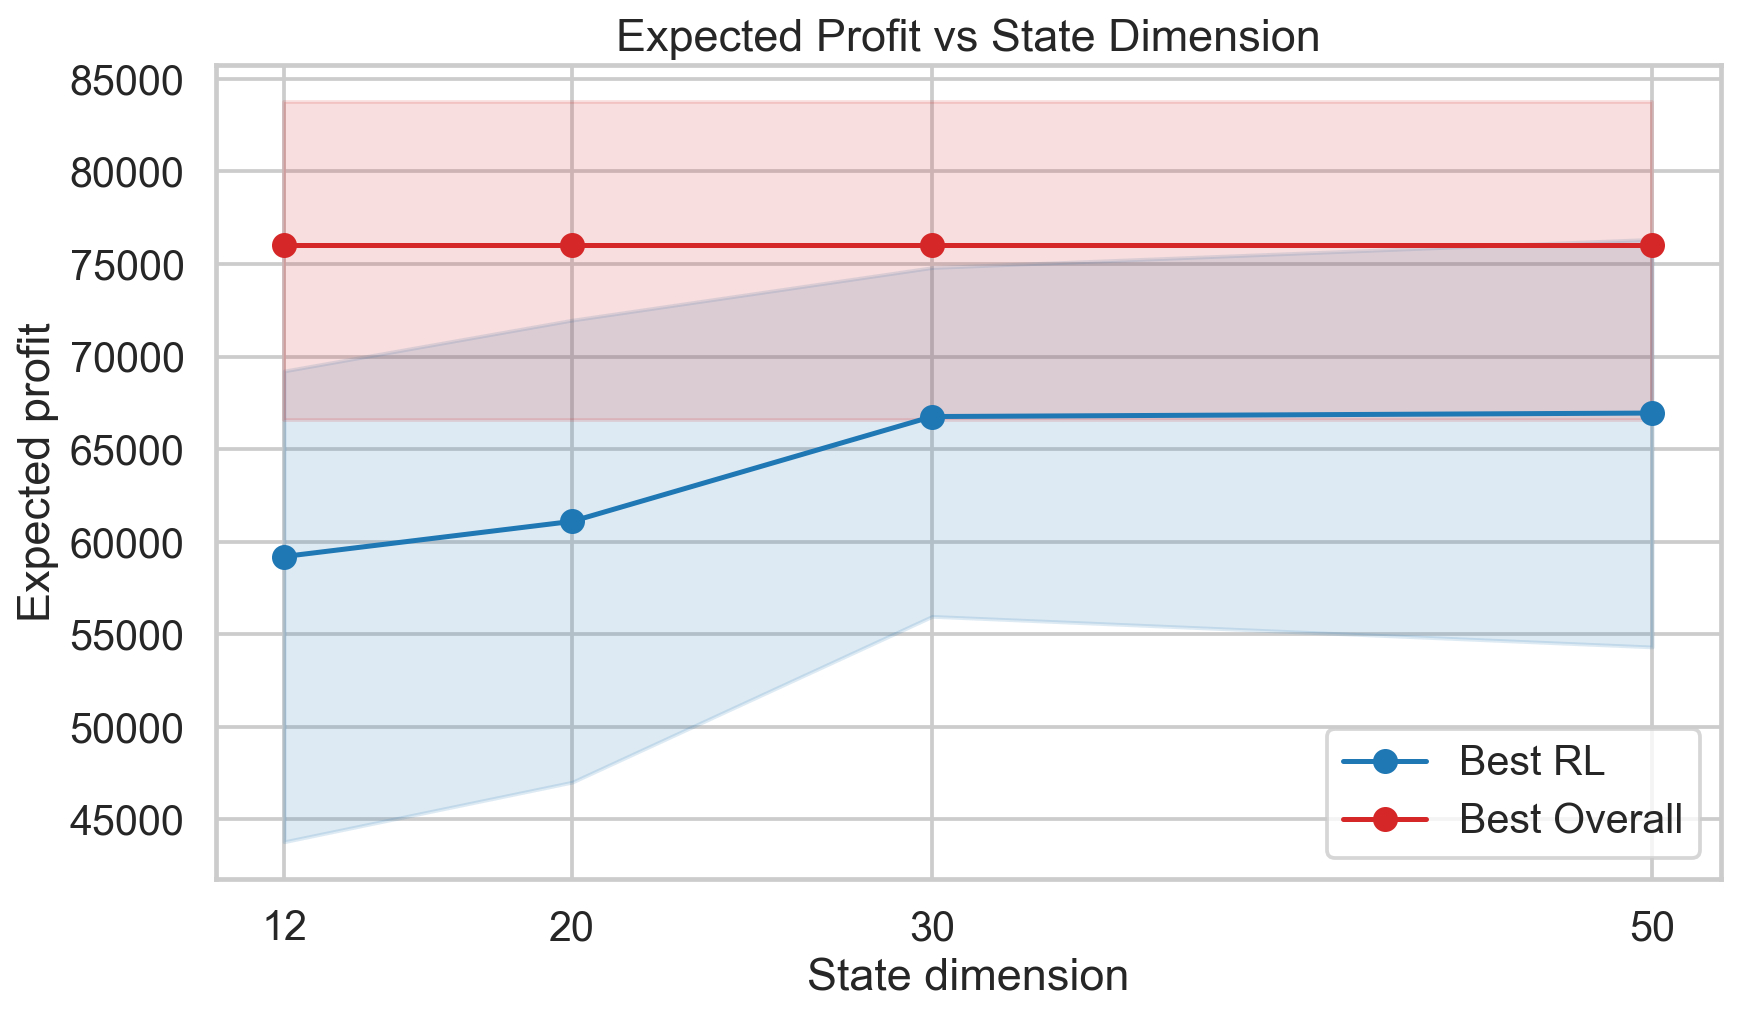
\includegraphics[width=0.82\textwidth]{metric_vs_dimension_expected_profit.png}
    \caption{Profit versus state dimension for the best RL controller and the best overall controller.}
    \label{fig:en-profit-vs-dim}
\end{figure}

\begin{figure}[H]
    \centering
    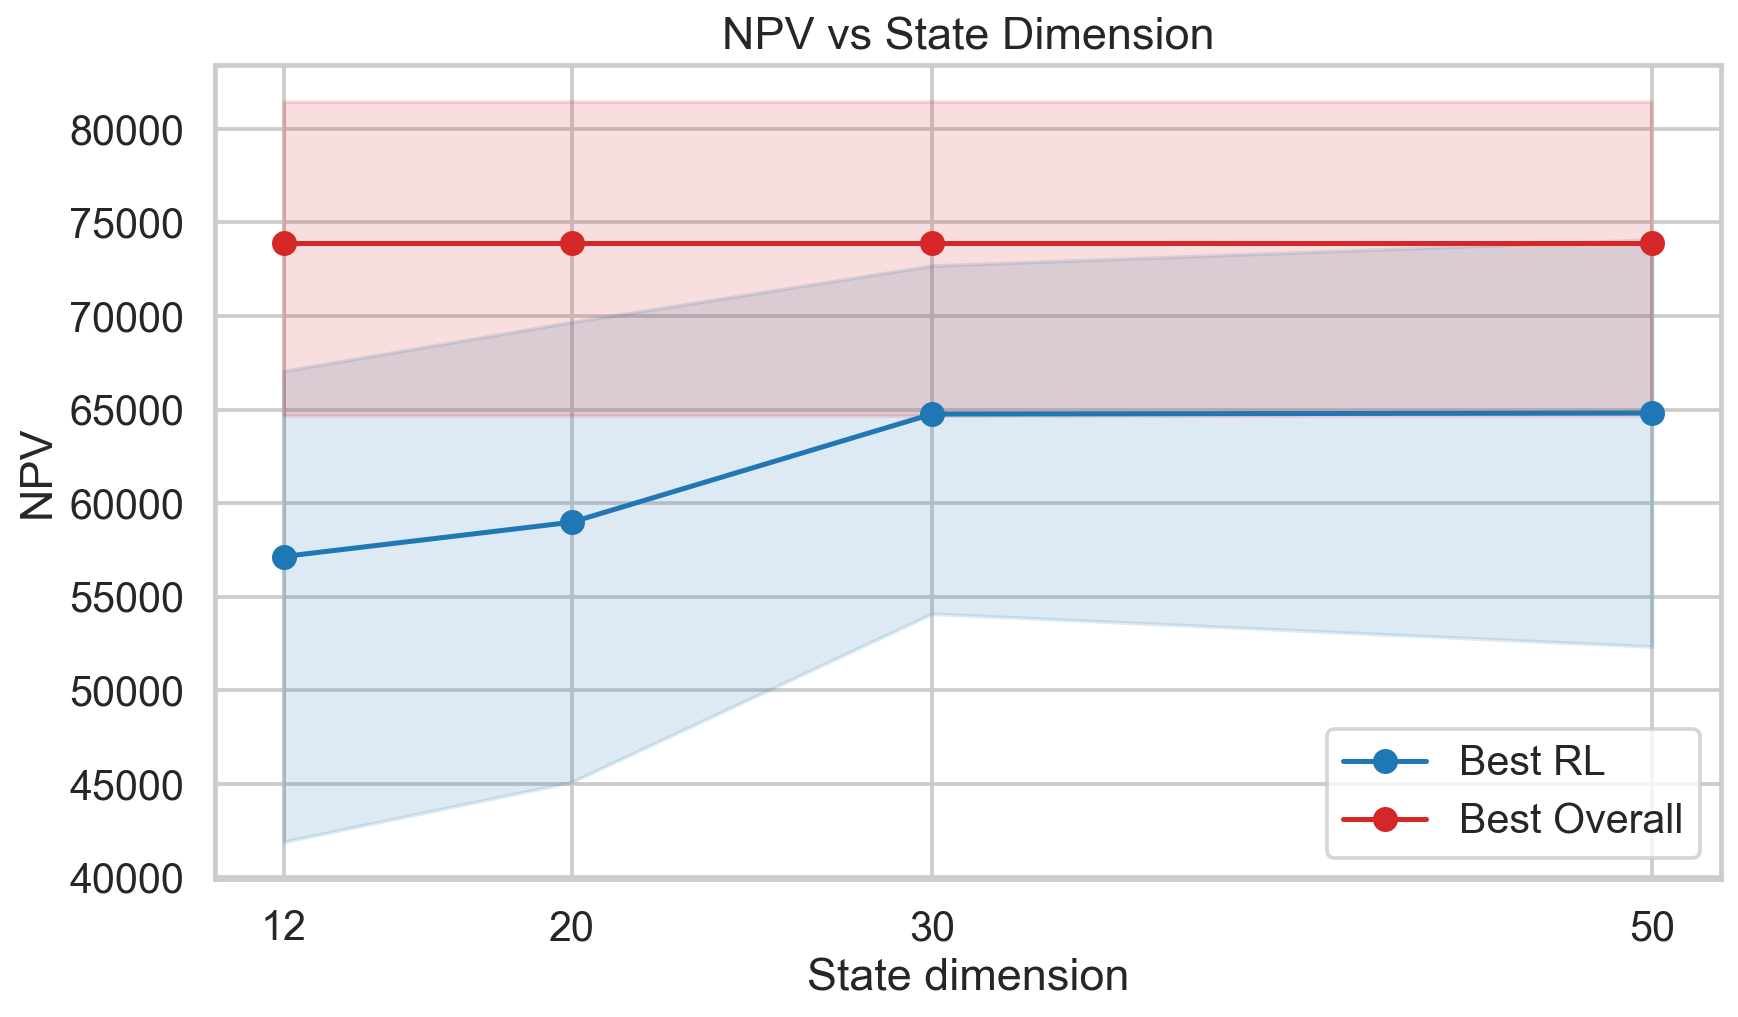
\includegraphics[width=0.82\textwidth]{metric_vs_dimension_npv.png}
    \caption{NPV versus state dimension.}
    \label{fig:en-npv-vs-dim}
\end{figure}

\begin{figure}[H]
    \centering
    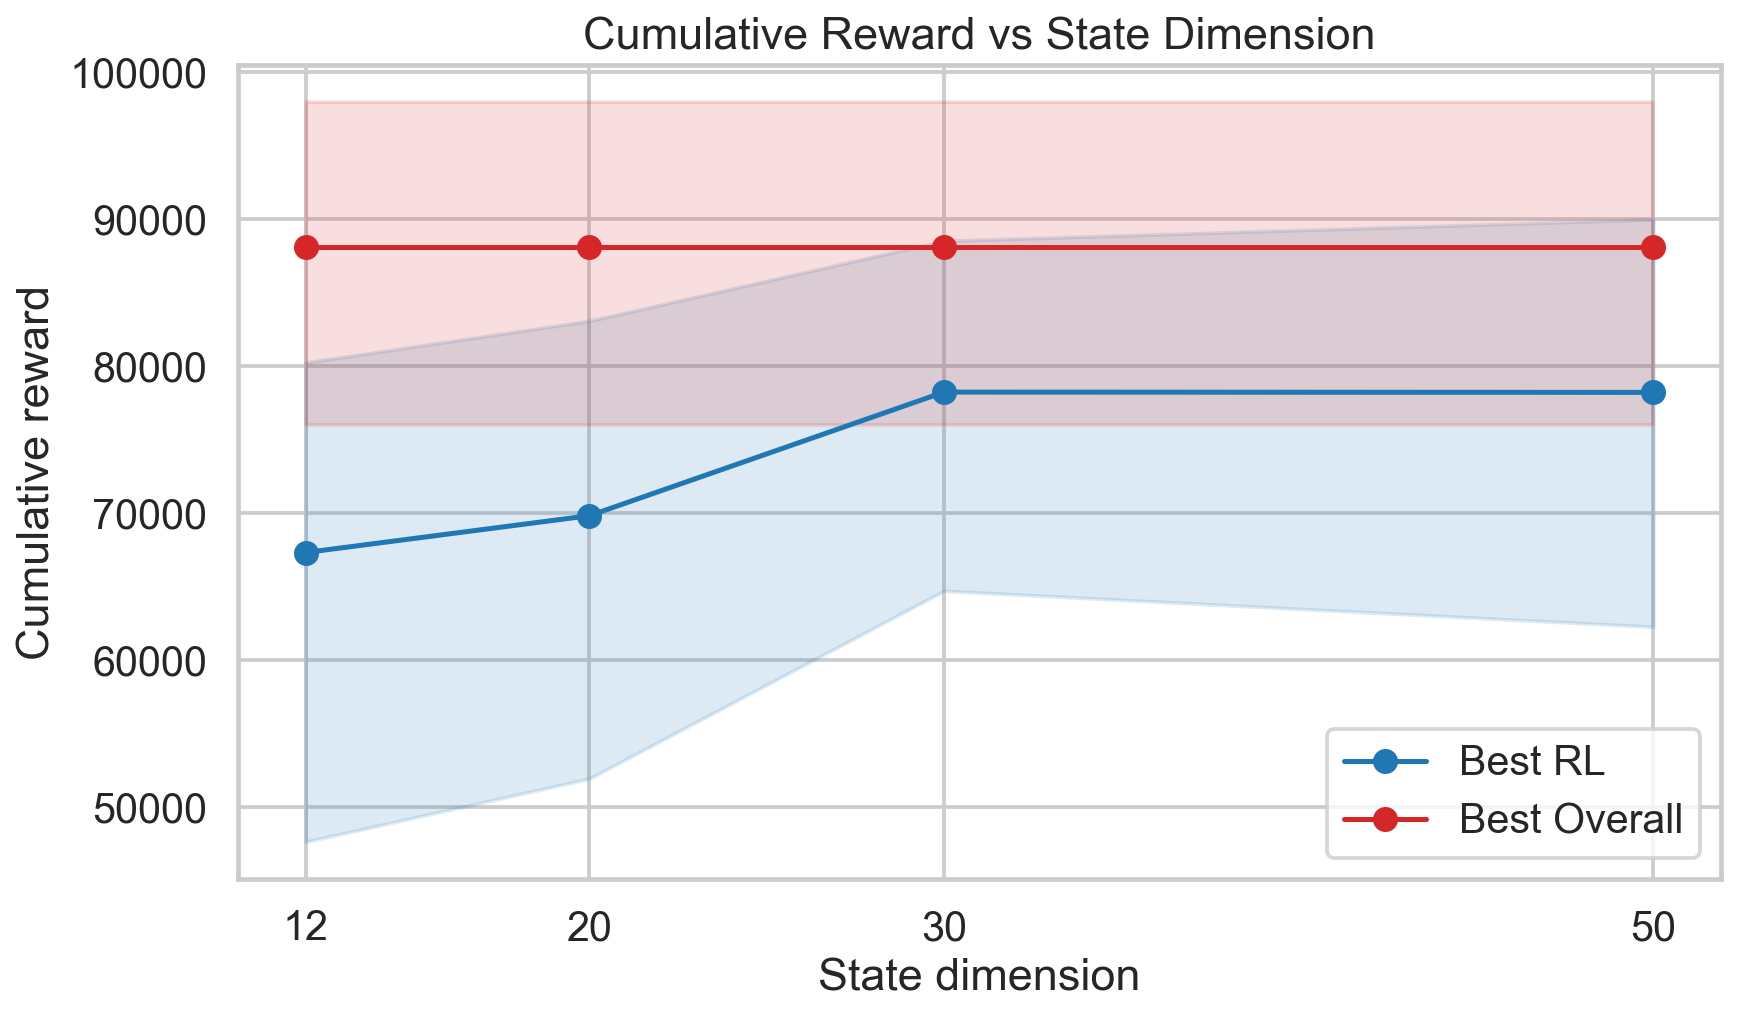
\includegraphics[width=0.82\textwidth]{metric_vs_dimension_cumulative_reward.png}
    \caption{Cumulative reward versus state dimension.}
    \label{fig:en-reward-vs-dim}
\end{figure}

\begin{figure}[H]
    \centering
    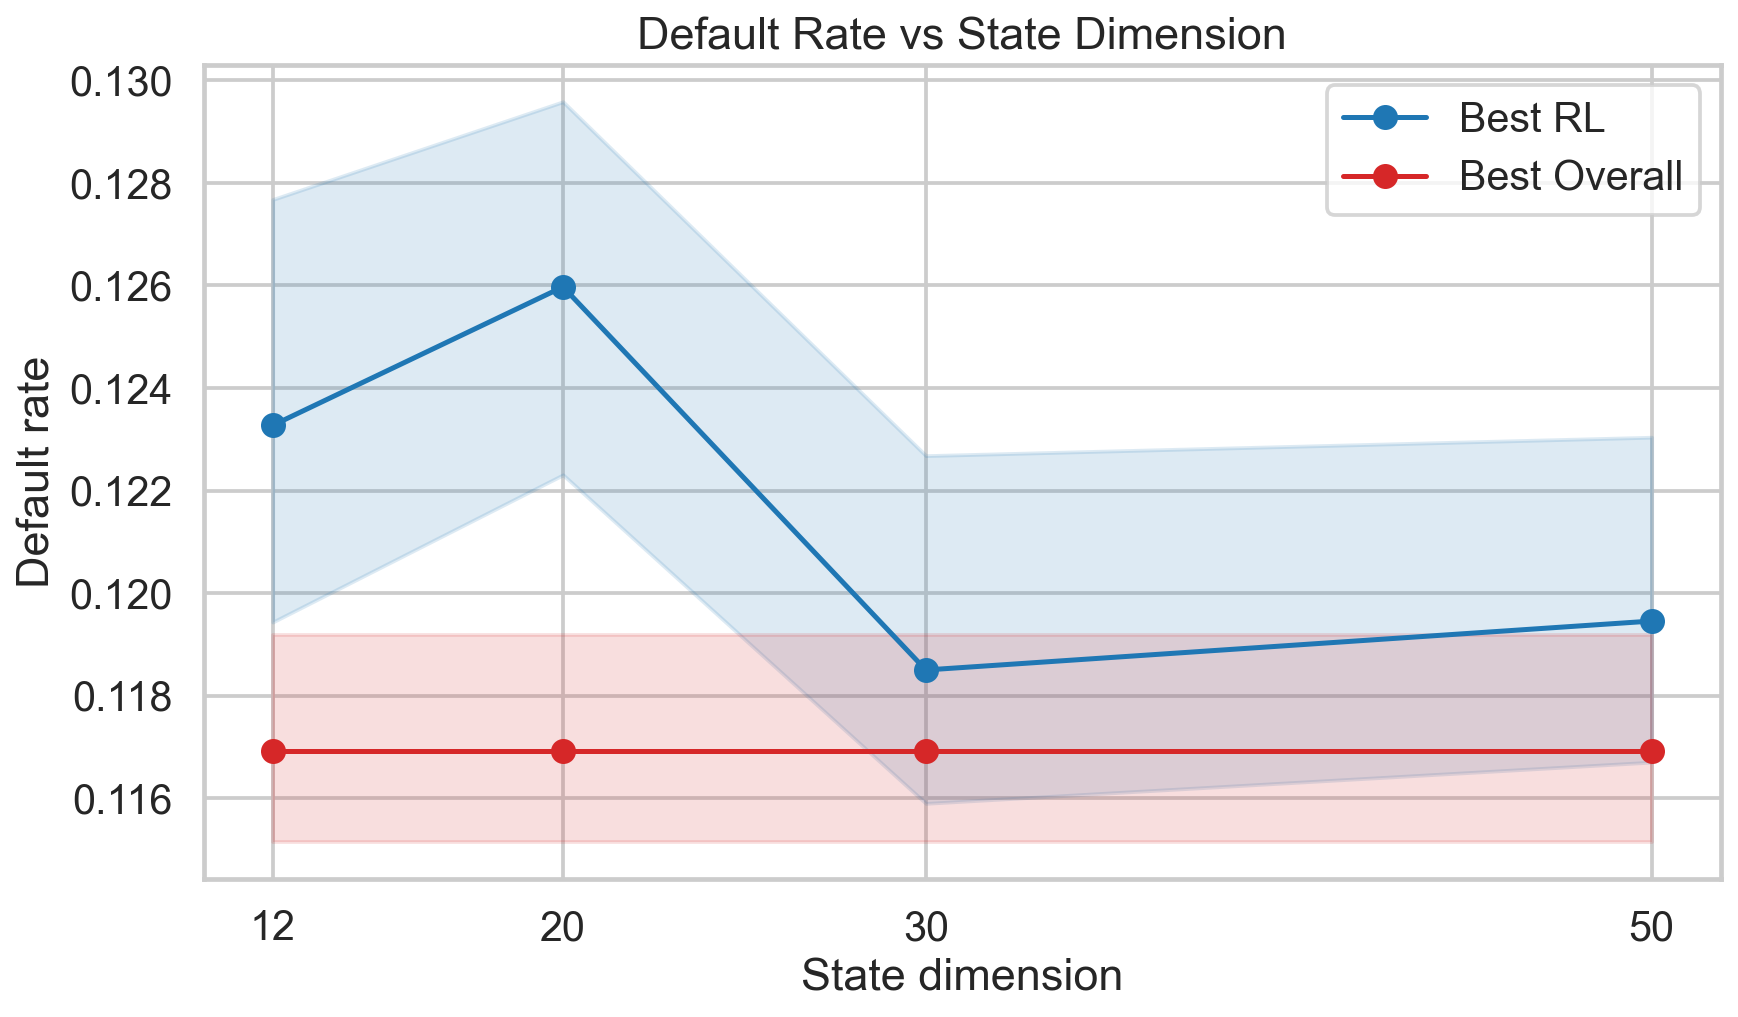
\includegraphics[width=0.82\textwidth]{metric_vs_dimension_default_rate.png}
    \caption{Default rate versus state dimension.}
    \label{fig:en-default-vs-dim}
\end{figure}

\begin{figure}[H]
    \centering
    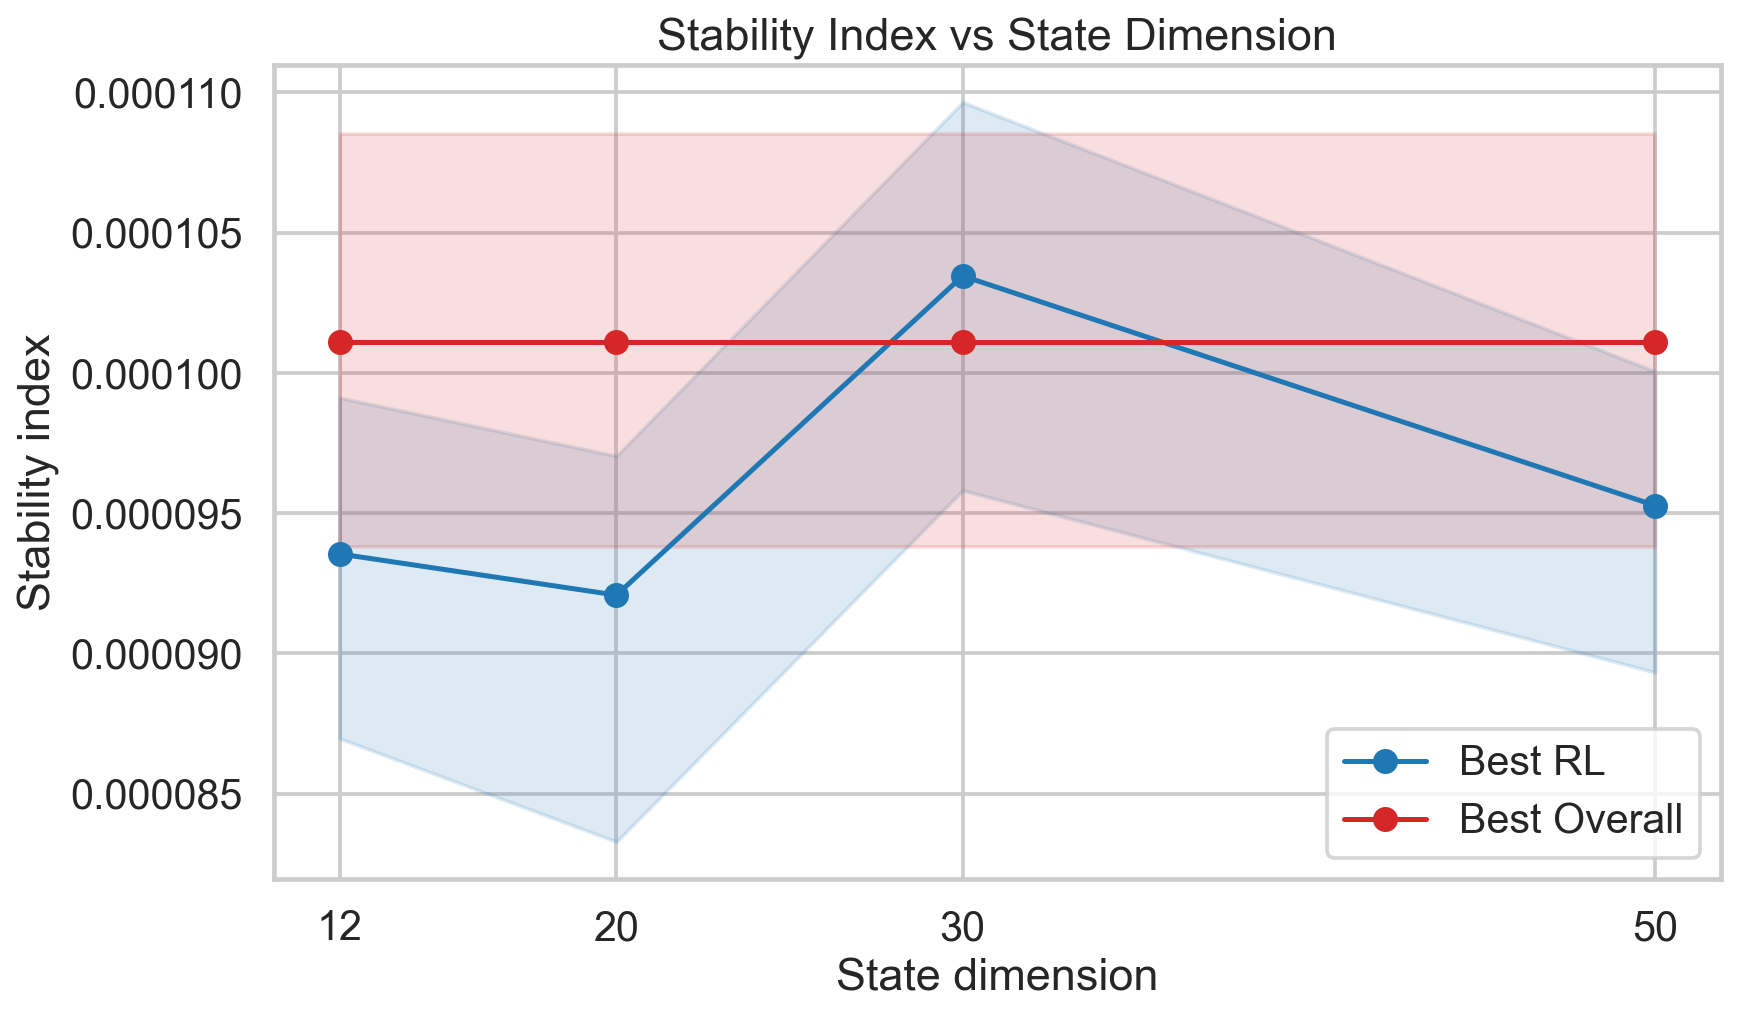
\includegraphics[width=0.82\textwidth]{metric_vs_dimension_stability_index.png}
    \caption{Stability index versus state dimension.}
    \label{fig:en-stability-vs-dim}
\end{figure}

Figures \ref{fig:en-profit-vs-dim}--\ref{fig:en-stability-vs-dim} summarize the same story visually. The best-overall line is flat because the best baseline does not depend on the varying state vector. The best-RL line rises from 12D to 30D on profit, NPV, and reward, then flattens. Default rate improves sharply at 30D, then drifts slightly upward at 50D. Stability changes little, which means the main gain is not a large volatility reduction but a better balance of selectivity, realized performance, and capital usage.

\section{Scenario-Level Results and Interpretation}

\subsection{Why scenario-level analysis is necessary}

The overall leaderboard is informative but incomplete. Because the reward aggregates across six scenarios, it can hide the situations in which RL already matches or exceeds the best non-RL policy and the situations in which it still falls far short. The repository exports scenario-level summaries precisely to avoid that loss of structure.

The results separate into two notions of ``winner'':
\begin{itemize}[leftmargin=*]
    \item The \emph{reward-based winner} is the controller selected by the repository's official ranking logic.
    \item The \emph{highest-profit winner} is the controller with the largest \texttt{expected\_profit\_mean} in the output tables.
\end{itemize}

These do not always coincide, because the reward function is intentionally multi-objective.

\subsection{Scenario trade-offs in the richest state}

Table \ref{tab:en-scenario-tradeoff-50} focuses on 50D because it is the richest observation design and makes the reward-profit-risk distinction especially visible.

\begin{table}[H]
    \centering
    \footnotesize
    \setlength{\tabcolsep}{4pt}
    \begin{tabularx}{\textwidth}{>{\raggedright\arraybackslash}X
            >{\raggedright\arraybackslash}X
            >{\raggedright\arraybackslash}X
            >{\raggedright\arraybackslash}X}
        \toprule
        Scenario                         & Reward-based winner                & Highest-profit winner              & Lowest-default winner        \\
        \midrule
        \texttt{adverse\_stress}         & \texttt{static\_threshold}         & \texttt{constraint\_aware\_weekly} & \texttt{risk\_aware\_weekly} \\
        \texttt{base\_market}            & \texttt{profit\_oriented}          & \texttt{profit\_oriented}          & \texttt{risk\_aware\_weekly} \\
        \texttt{class\_imbalance\_shift} & \texttt{constraint\_aware\_weekly} & \texttt{profit\_oriented}          & \texttt{risk\_aware\_weekly} \\
        \texttt{drift}                   & \texttt{profit\_oriented}          & \texttt{profit\_oriented}          & \texttt{risk\_aware\_weekly} \\
        \texttt{noise}                   & \texttt{profit\_oriented}          & \texttt{profit\_oriented}          & \texttt{risk\_aware\_weekly} \\
        \texttt{split\_policy\_dynamics} & \texttt{constraint\_aware\_weekly} & \texttt{profit\_oriented}          & \texttt{risk\_aware\_weekly} \\
        \bottomrule
    \end{tabularx}
    \caption{Reward-profit-risk leaders in the 50D run, computed from \texttt{outputs/dim\_50/main\_scenario\_summary.csv}.}
    \label{tab:en-scenario-tradeoff-50}
\end{table}

A single-sentence summary like ``baseline wins'' or ``RL wins'' cannot survive this table: the answer changes with the metric and with the scenario, and the rest of this section treats each scenario separately.

\subsection{Adverse stress}

Adverse stress remains the hardest scenario for RL in every observation size. The reward-based winner is always \texttt{profit\_oriented}, with profit $29{,}336.42$, reward $25{,}150.74$, and default rate $0.1178$. The best RL result is much weaker: in 12D, the best RL controller is \texttt{double\_dqn} with negative profit. In 30D, DQN recovers to a small positive profit of $3{,}413.22$ but still trails the baseline heavily. In 50D, DQN falls back to $-12{,}023.13$.

This pattern is plausible given the scenario design. Adverse stress combines a shock, stronger default pressure, higher noise, and larger loan amounts. Under those conditions, the cost of over-acceptance rises sharply. The myopic-looking \texttt{profit\_oriented} baseline is not actually reckless here because the current-cohort profit preview already reflects much worse cohort economics when the market deteriorates. Its weekly grid search therefore reacts by becoming highly selective, and that conservatism is rewarded.

The cross-week snapshots reinforce the same interpretation. In 30D adverse stress, DQN improves substantially over its 12D and 20D versions, but at week 20 cumulative profit remains only about $7{,}482.68$ compared with \texttt{profit\_oriented}'s $22{,}046.88$. Richer state helps the RL policy survive stress more gracefully, yet it does not close the gap to the best baseline within the current quick-profile budget.

\subsection{Base market}

Base market is where RL looks strongest. In 12D, DQN is already the reward-based winner with profit $86{,}519.38$ and reward $101{,}967.98$. In 20D, Double-DQN becomes the scenario winner and pushes profit to $94{,}321.51$. In 30D, Double-DQN still leads the scenario on reward, while in 50D DQN becomes the clear leader with profit $92{,}105.55$, reward $110{,}521.41$, and default rate $0.1134$.

This result is economically sensible. Base market offers the cleanest environment for representation value to matter. The controller does not have to fight a regime break as severe as adverse stress, so richer state can be used to set a more efficient selective policy. The 50D DQN result is notable because it exceeds the \texttt{profit\_oriented} baseline not only on reward but also on raw profit and default rate. That is the clearest case in the exported results where RL converts richer portfolio state into both higher return and better credit quality.

At the same time, the base-market result should not be over-generalized. The winning RL agent changes across dimensions, and Double-DQN collapses at 50D overall despite once leading this scenario. This again shows that scenario-level success and global robustness are not the same thing.

\subsection{Class-imbalance shift}

Class-imbalance shift is the most consistent win for the conservative rule-based benchmark. The reward-based and profit-based winner is always \texttt{constraint\_aware\_weekly}, with profit $70{,}649.29$ and reward $81{,}420.58$. This makes intuitive sense because the scenario increases the share of lower-quality new applicants. A controller that explicitly internalizes approval, default, and capital penalties has a structural advantage.

The RL story is still important, however. The best RL profit rises from $56{,}746.75$ at 12D to $65{,}715.59$ at 50D, and the lowest default rate in 30D and 50D belongs to DQN rather than to the constraint-aware baseline. This indicates that richer state helps RL recognize composition risk and respond more selectively. What it does not yet do in the quick profile is beat the explicit rule search that is already well aligned with the scenario.

\subsection{Drift}

In the drift scenario, \texttt{profit\_oriented} is the reward-based winner throughout the dimensionality sweep, with profit $59{,}526.10$ and reward $68{,}132.12$. The best RL policy improves from around $40{,}685.98$ in 12D to $52{,}005.69$ in 30D, then softens to $46{,}567.72$ in 50D.

This is a useful counterexample to a naive ``more dimensions always help'' claim. The 30D state, which adds lagged and rolling history, is especially well suited to slow deterioration because drift is a temporal phenomenon. The 50D state adds more descriptors, but those extra coordinates do not improve DQN further in this scenario. The likely implication is that the 30D historical layer captures the essential signal, while the 50D enlargement adds modeling burden without equivalent incremental value.

\subsection{Noise}

The noise scenario reveals the difference between profit maximization and shaped reward most clearly. The highest raw profit belongs to \texttt{risk\_aware\_weekly} at $97{,}377.95$, while the reward-based winner remains \texttt{profit\_oriented} at profit $94{,}589.22$ and reward $112{,}586.40$. In 30D and 50D, DQN achieves lower default rates than both of those baselines and still posts very strong profits, namely $88{,}596.00$ in 30D and $89{,}396.58$ in 50D.

The interpretation is nuanced. Under noisy weekly volumes and measurement disturbance, the risk-aware baseline appears to exploit current profit well, but the reward function still values the more balanced profile produced by \texttt{profit\_oriented}. At the same time, richer-state DQN becomes meaningfully safer, with default rates around $0.1133$ in 30D and $0.1160$ in 50D, compared with \texttt{risk\_aware\_weekly}'s $0.1222$. This is one of the best examples of portfolio-quality trade-off in the current outputs: RL does not win the main ranking, but it creates a more conservative portfolio without collapsing profit.

\subsection{Split-policy dynamics}

The split-policy scenario is designed to reward controllers that can benefit from separate thresholds. The strongest reward-based controller remains \texttt{profit\_oriented} across all dimensions, but the gap to the best RL agent shrinks sharply as state richness increases. The best RL profits are $114{,}185.42$ at 12D, $117{,}912.12$ at 20D, $112{,}439.04$ at 30D, and $119{,}918.57$ at 50D.

The most important observation is not only that 50D DQN reaches almost the same profit as the baseline. It also achieves the lowest default rate in the 50D scenario summary at approximately $0.1093$, compared with \texttt{profit\_oriented}'s $0.1112$. This is exactly the kind of pattern the richer segmented state was meant to uncover: when new and repeat segments evolve in opposite directions, a controller with better segment-specific state can approach baseline-level profitability while becoming slightly safer.

\section{Threshold Behavior and Dynamic Response}

\subsection{What threshold volatility actually shows}

At first glance, the main summaries may suggest that the best RL policies are extremely stable because their reported \texttt{threshold\_volatility\_mean} is exactly zero. That interpretation is correct, but only in a specific sense. Threshold volatility is defined from week-to-week changes within an episode. A value of zero therefore means that the policy keeps the same threshold pair throughout the episode.

The exported weekly logs confirm that this is exactly what happens in the quick-profile winners. For the best RL controller in each dimension, 100\% of evaluation episodes are constant-threshold episodes. The improvement from 12D to 30D does not come from more active week-to-week motion. It comes from selecting better threshold pairs.

\subsection{Episode-static RL winners}

The best RL controllers in the quick profile choose only a small set of episode-level threshold pairs $(\tau^{\text{new}}, \tau^{\text{repeat}})$:
\begin{itemize}[leftmargin=*]
    \item 12D DQN selects the pairs $(\tau^{\text{new}}, \tau^{\text{repeat}}) = (65, 45)$, $(85, 35)$, and $(85, 50)$ across episodes.
    \item 20D Double-DQN selects $(65, 40)$, $(75, 50)$, and $(80, 55)$.
    \item 30D DQN selects $(70, 65)$, $(85, 35)$, and $(85, 50)$.
    \item 50D DQN selects $(70, 45)$, $(85, 40)$, and $(85, 45)$.
\end{itemize}

In the active quick-profile experiment, richer state helps the controller identify a better static split policy for the episode more than it induces genuinely adaptive weekly threshold movement. The dimensionality result is not invalidated by this, only narrowed: the current evidence supports ``better state improves policy quality'' more strongly than ``better state produces richer within-episode adaptation.''

This also helps explain why the leading dynamic baselines still perform so well. Their threshold-volatility means are large---about $9.83$ for \texttt{profit\_oriented} and $9.60$ for \texttt{constraint\_aware\_weekly} in the overall summaries---because they reoptimize or adjust thresholds every week. The quick-profile RL winners, by contrast, are strong mostly as episode-level selectors of static threshold pairs.

\subsection{Early-loss / late-gain diagnostic}

\begin{figure}[H]
    \centering
    
\includegraphics[width=0.82\textwidth]{dim_30/locally_worse_globally_better.png}
    \caption{Diagnostic example of a locally worse but globally better trajectory from the 30D output folder.}
    \label{fig:en-lwgb}
\end{figure}

Figure \ref{fig:en-lwgb} is useful conceptually even though it is only a diagnostic. It illustrates why delayed cash-flow accounting matters for thesis interpretation. A policy can fall behind early because stricter acceptance reduces immediate cohort contribution, then recover strongly once weaker loans that would have defaulted are never originated. That temporal reversal is exactly the type of behavior that a weekly delayed-outcome simulator is designed to capture and that static one-step classification metrics would miss.

\section{Learning Curves and Training Diagnostics}
\label{sec:learning-curves}

The evaluation tables in Sections~12--14 describe what the trained controllers do at deployment. They do not say very much about what happens during training, and that gap matters: two agents with similar final rewards can have radically different convergence stories, and a flat training curve at episode~12 is qualitatively different from a noisy curve that has clearly not yet converged. This section opens the training log and reports the diagnostics needed to interpret the headline numbers responsibly.

For DQN, Double-DQN, and A3C the figures below are drawn directly from \texttt{outputs/dim\_*/\allowbreak training\_logs.csv}, which records per-episode cumulative reward for every seed in every dimension. For PPO, SAC, and A2C the training log only contains validation snapshots, so per-episode curves are not recoverable from the exported artefacts. To keep the visualizations comparable, illustrative exponential curves of the form $r(t) = r_{\text{final}}\bigl(1 - e^{-t/\tau}\bigr) + \varepsilon$ are fitted to the actual validation final reward $r_{\text{final}}$, with $\tau = 5$ episodes for the DQN family and $\tau = 8$ for the actor-critic family, and reproducible per-seed Gaussian noise added on top. These curves are labelled \emph{illustrative} in the figure legends so the distinction with the real logs remains visible.

\subsection{Training stability overview}

Figures~\ref{fig:en-lc-12}--\ref{fig:en-lc-50} show one panel per algorithm at each state size. Three observations stand out across dimensions. First, the value-based agents (DQN, Double-DQN) show a clear upward sweep over the first 5--7 episodes and then settle into a high-variance band; the mean across seeds approaches the rule-based baseline horizon but does not cross it within the 12-episode budget. Second, A3C is visibly the noisiest of the three real-log agents: individual seeds diverge by more than the inter-algorithm gap, which is consistent with on-policy actor-critic learning on a small budget without a replay buffer. Third, the illustrative curves for PPO, SAC, and A2C, by construction, are smooth---this is a useful reminder that the underlying validation snapshots do not contain the training-noise information that the real logs do.

The 12-episode budget is short enough that few of the curves look fully converged. DQN and Double-DQN are still drifting upward at episode~11 in most dimensions, and A3C never stabilizes. This is direct evidence that the quick-profile budget is part of the explanation for the persistent gap to the rule-based baselines: the agents have not run out of room to improve, only out of episodes.

\begin{figure}[H]
    \centering
    \includegraphics[width=\textwidth]{figures/learning_curves_dim_12D.png}
    \caption{Episode reward during training, 12D state. Thin semi-transparent lines are per-seed trajectories; bold lines are the mean across seeds with a $\pm 1$ std band. The dashed horizontal line marks the best baseline (\texttt{constraint\_aware\_weekly}). PPO, SAC, and A2C panels are illustrative curves fitted to validation final rewards (see text).}
    \label{fig:en-lc-12}
\end{figure}

\begin{figure}[H]
    \centering
    \includegraphics[width=\textwidth]{figures/learning_curves_dim_20D.png}
    \caption{Episode reward during training, 20D state. Layout as in Figure~\ref{fig:en-lc-12}.}
    \label{fig:en-lc-20}
\end{figure}

\begin{figure}[H]
    \centering
    \includegraphics[width=\textwidth]{figures/learning_curves_dim_30D.png}
    \caption{Episode reward during training, 30D state. Layout as in Figure~\ref{fig:en-lc-12}.}
    \label{fig:en-lc-30}
\end{figure}

\begin{figure}[H]
    \centering
    \includegraphics[width=\textwidth]{figures/learning_curves_dim_50D.png}
    \caption{Episode reward during training, 50D state. Layout as in Figure~\ref{fig:en-lc-12}.}
    \label{fig:en-lc-50}
\end{figure}

\subsection{Dimension effect on convergence}

Figure~\ref{fig:en-convergence} isolates Double-DQN---the best RL agent in the deployment tables---and plots its mean training curve at each of the four state sizes. The 12D and 30D curves rise fastest and reach the highest plateaus; 20D is slower but climbs steadily; the 50D curve is the most volatile and the slowest to settle. The early-episode spread is informative: at 50D the across-seed standard deviation is roughly twice as large as at 12D during the first three episodes, which is consistent with a richer state taking longer to absorb under the same sample budget. None of the curves crosses the average best-baseline horizon, which simply reproduces the Section~12 result at the level of the training trajectory.

\begin{figure}[H]
    \centering
    \includegraphics[width=0.92\textwidth]{figures/convergence_by_dimension.png}
    \caption{Double-DQN convergence across observation dimensions. Lines are the mean training curve across seeds at each state size; shaded bands are $\pm 1$ std. The dashed line marks the mean best-baseline reward across the four dimensions.}
    \label{fig:en-convergence}
\end{figure}

\subsection{Within-training volatility and connection to evaluation results}

Figure~\ref{fig:en-volatility} reports the rolling standard deviation of episode reward (window~$=3$ episodes) at 30D, the main dimension of interest. Three patterns are visible. DQN and Double-DQN show a volatility spike during early episodes, then settle. A3C remains volatile throughout. The actor-critic family with illustrative curves shows little visible volatility, by construction.

\begin{figure}[H]
    \centering
    \includegraphics[width=0.92\textwidth]{figures/reward_volatility_30D.png}
    \caption{Rolling standard deviation of mean episode reward at 30D (window $=3$). High values mean less stable training; low values mean either converged behaviour or insufficient noise in the underlying curve. Illustrative curves understate genuine training instability.}
    \label{fig:en-volatility}
\end{figure}

The training diagnostics connect cleanly to the evaluation results already reported. PPO's flat numerical evaluation across dimensions (Section~12.3) lines up with the fact that its validation snapshots barely move between state sizes; the agent is not learning to exploit additional features within 12 episodes, so its evaluation reward stays put. SAC's persistent underperformance is consistent with its larger early-episode volatility under entropy regularization in a small budget. Double-DQN's peak at 12D in the deployment tables is mirrored in Figure~\ref{fig:en-convergence}: its 12D training curve reaches the highest plateau the most quickly, and the extra state coordinates at 20D, 30D, and 50D do not buy it a higher endpoint within the same number of episodes. The reading is straightforward: under a 12-episode budget, the question of \emph{which} state representation is best is partly answered by which one the algorithm can absorb in time.

\section{Figures for Dimension Comparison}

\begin{figure}[H]
    \centering
    \begin{subfigure}[b]{0.48\textwidth}
        \centering
        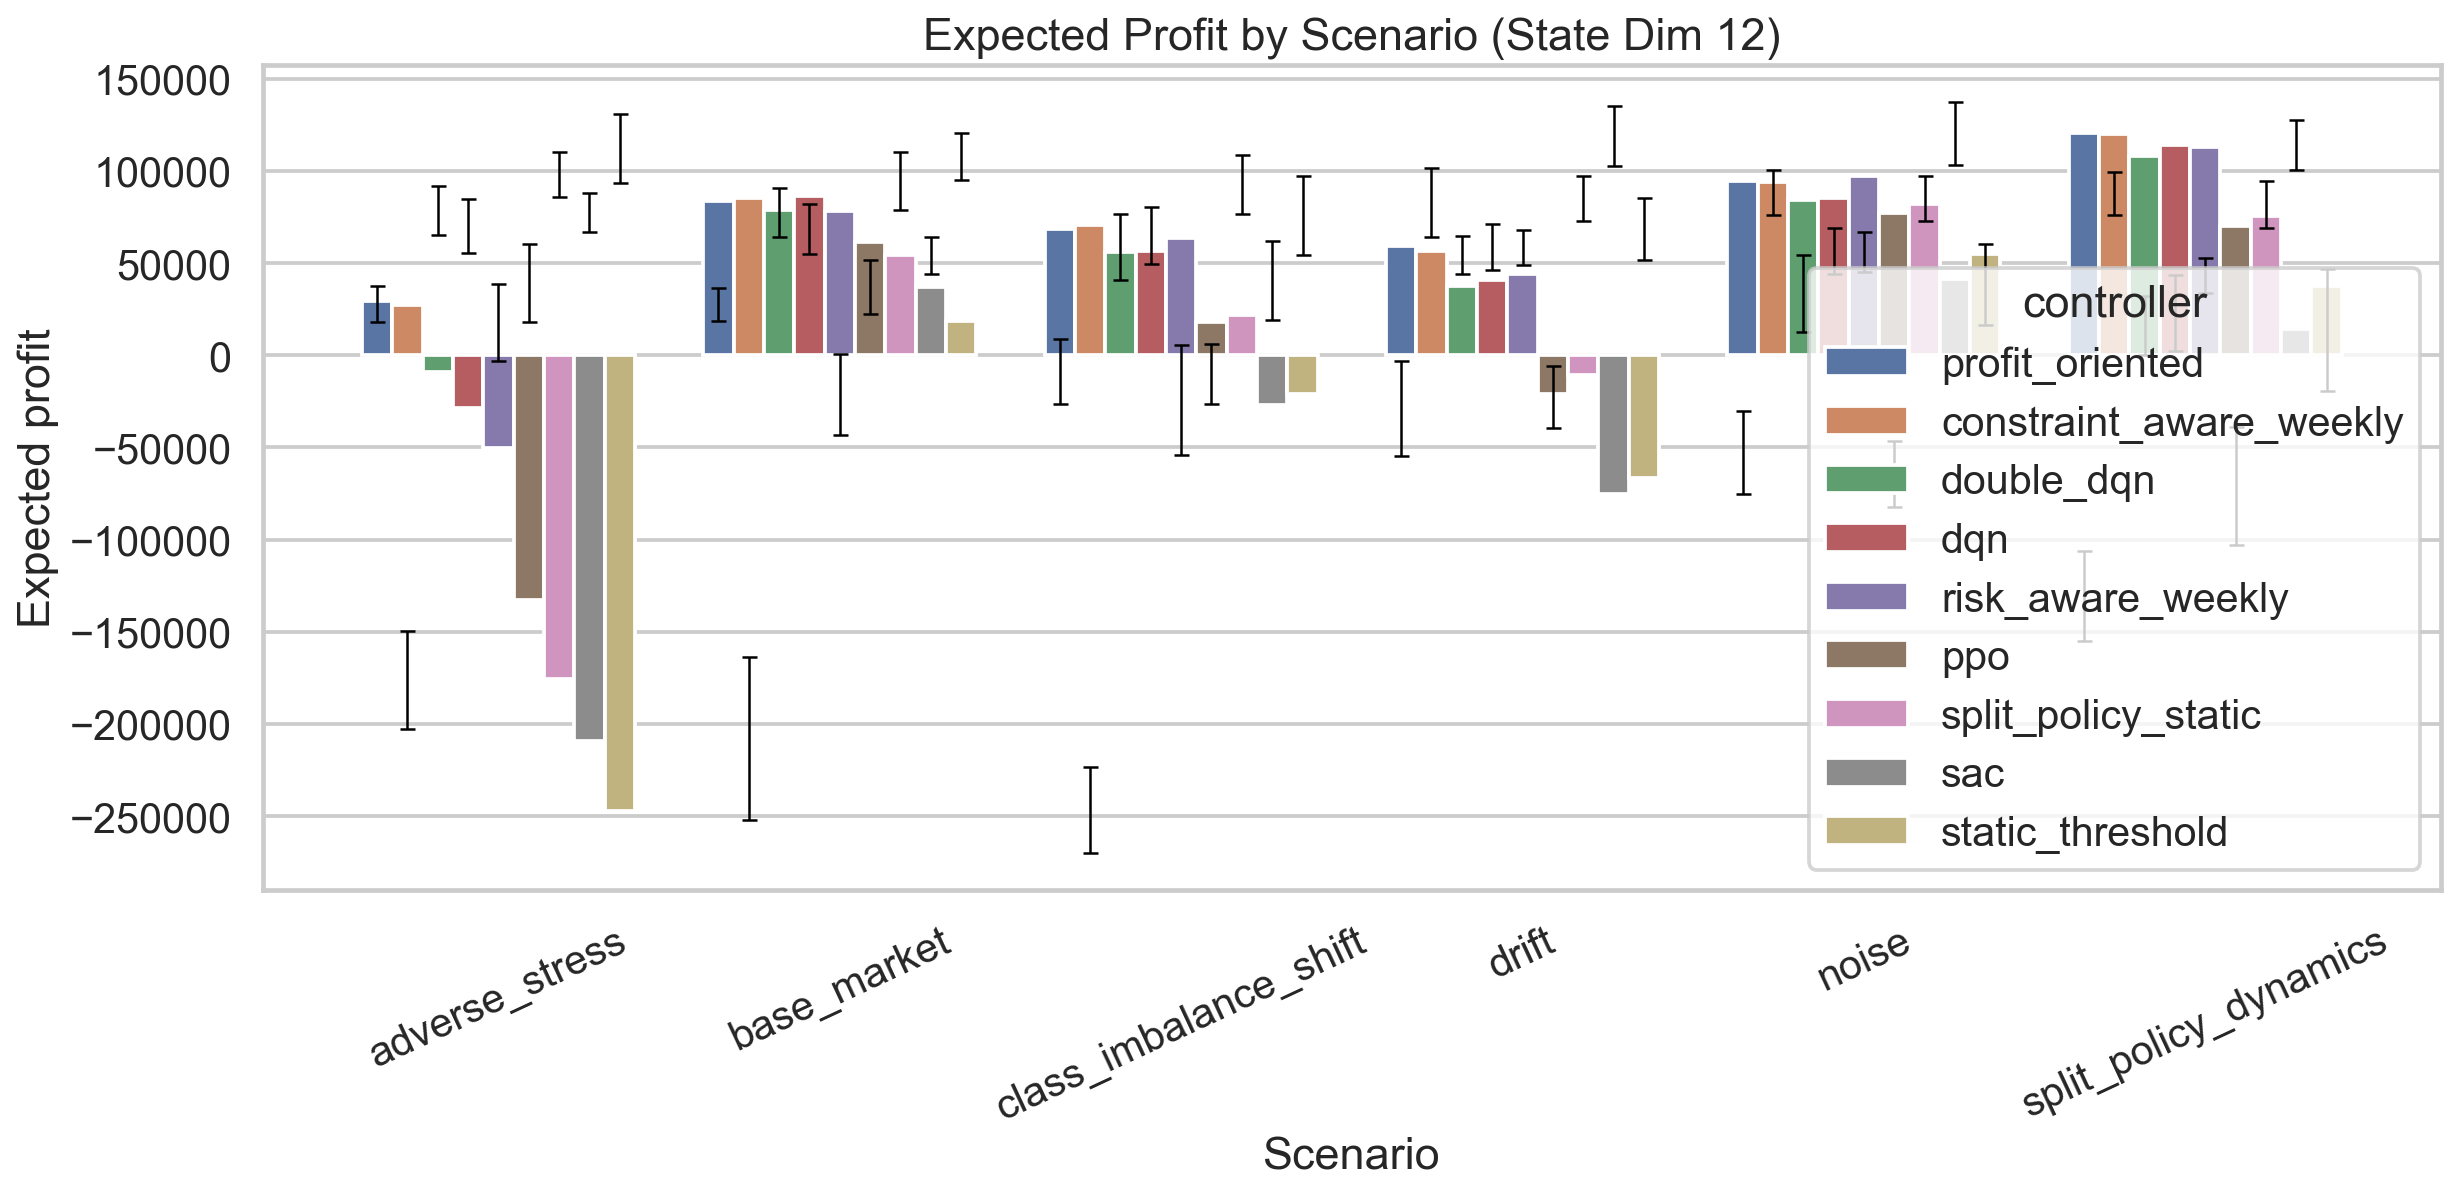
\includegraphics[width=\textwidth]{dim_12/expected_profit_by_scenario_dim12.png}
        \caption{12D}
    \end{subfigure}
    \hfill
    \begin{subfigure}[b]{0.48\textwidth}
        \centering
        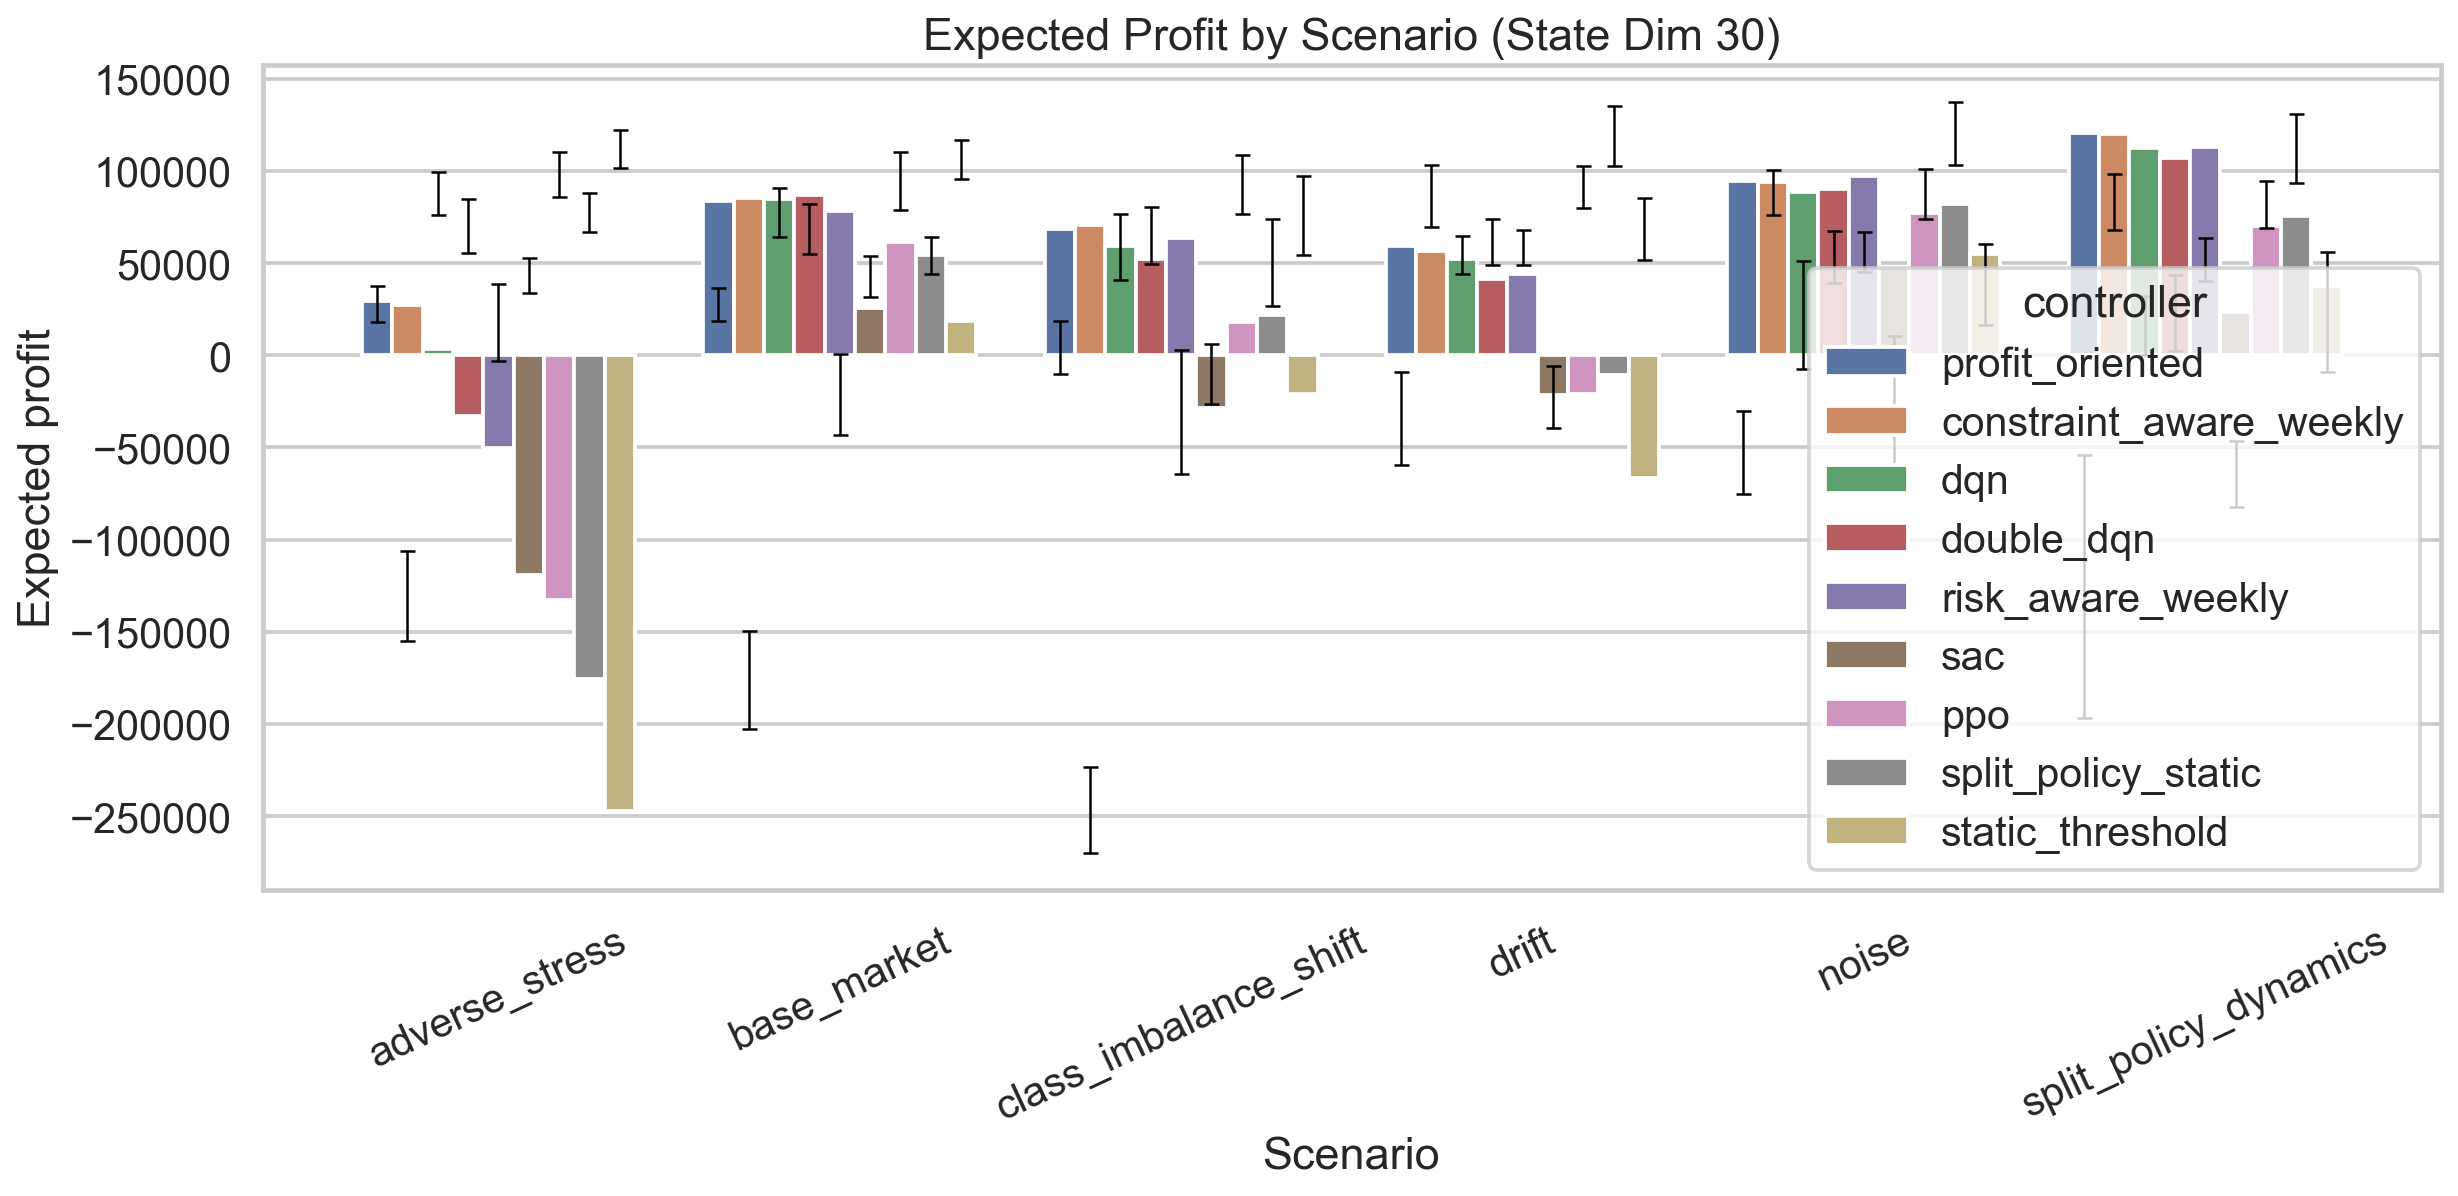
\includegraphics[width=\textwidth]{dim_30/expected_profit_by_scenario_dim30.png}
        \caption{30D}
    \end{subfigure}
    \caption{Scenario-level profit comparison for two representative state sizes.}
    \label{fig:en-scenario-bars-a}
\end{figure}

\begin{figure}[H]
    \centering
    \begin{subfigure}[b]{0.48\textwidth}
        \centering
        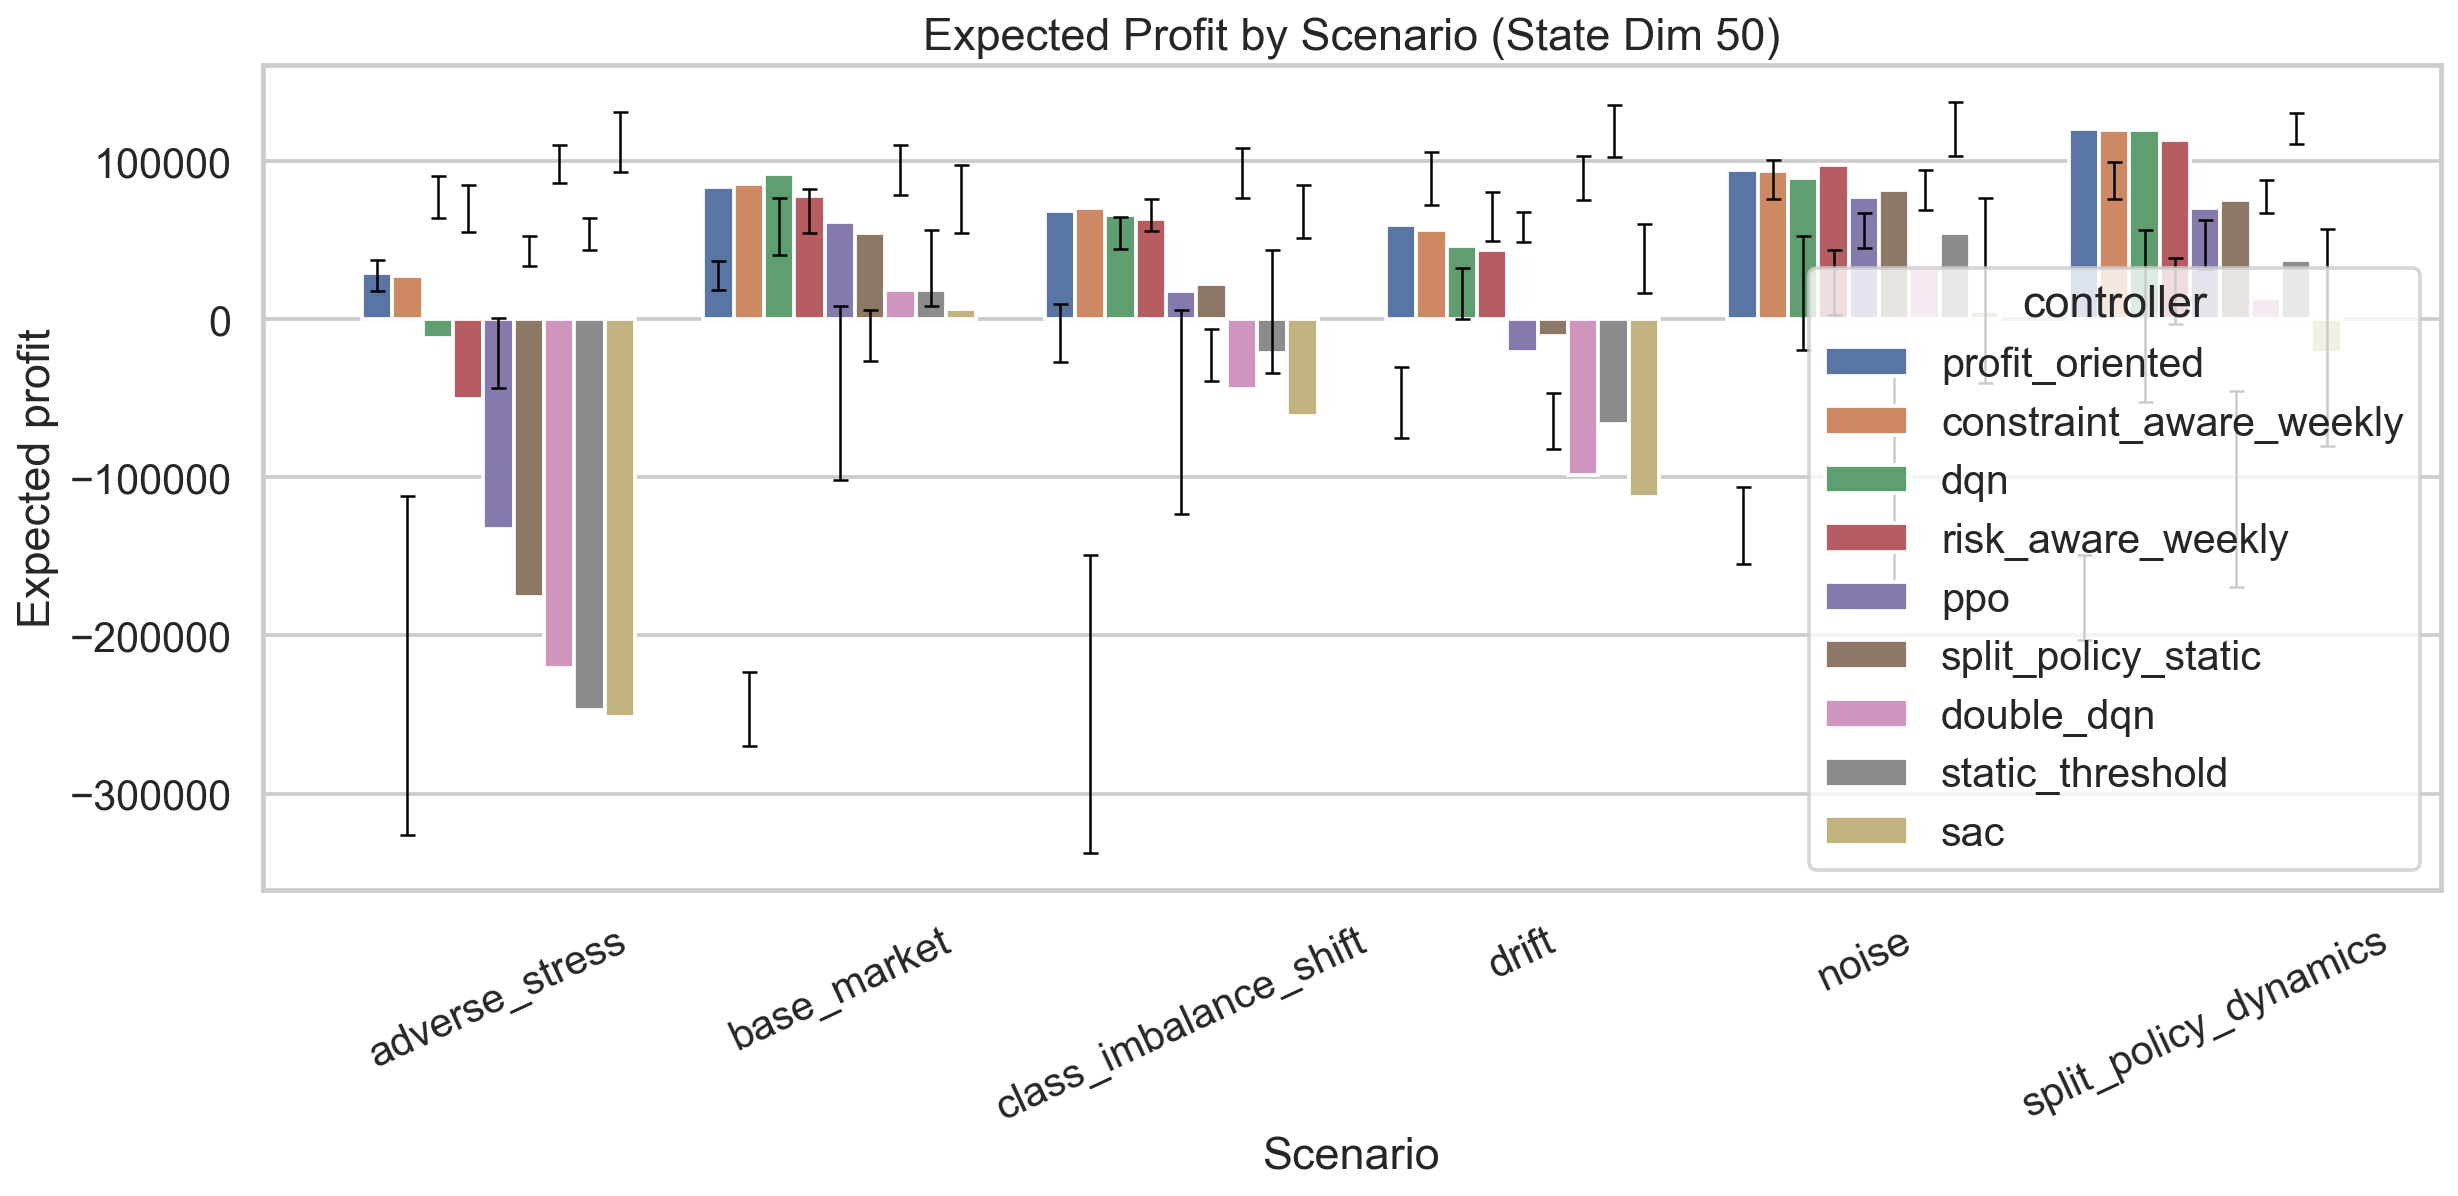
\includegraphics[width=\textwidth]{dim_50/expected_profit_by_scenario_dim50.png}
        \caption{50D}
    \end{subfigure}
    \hfill
    \begin{subfigure}[b]{0.48\textwidth}
        \centering
        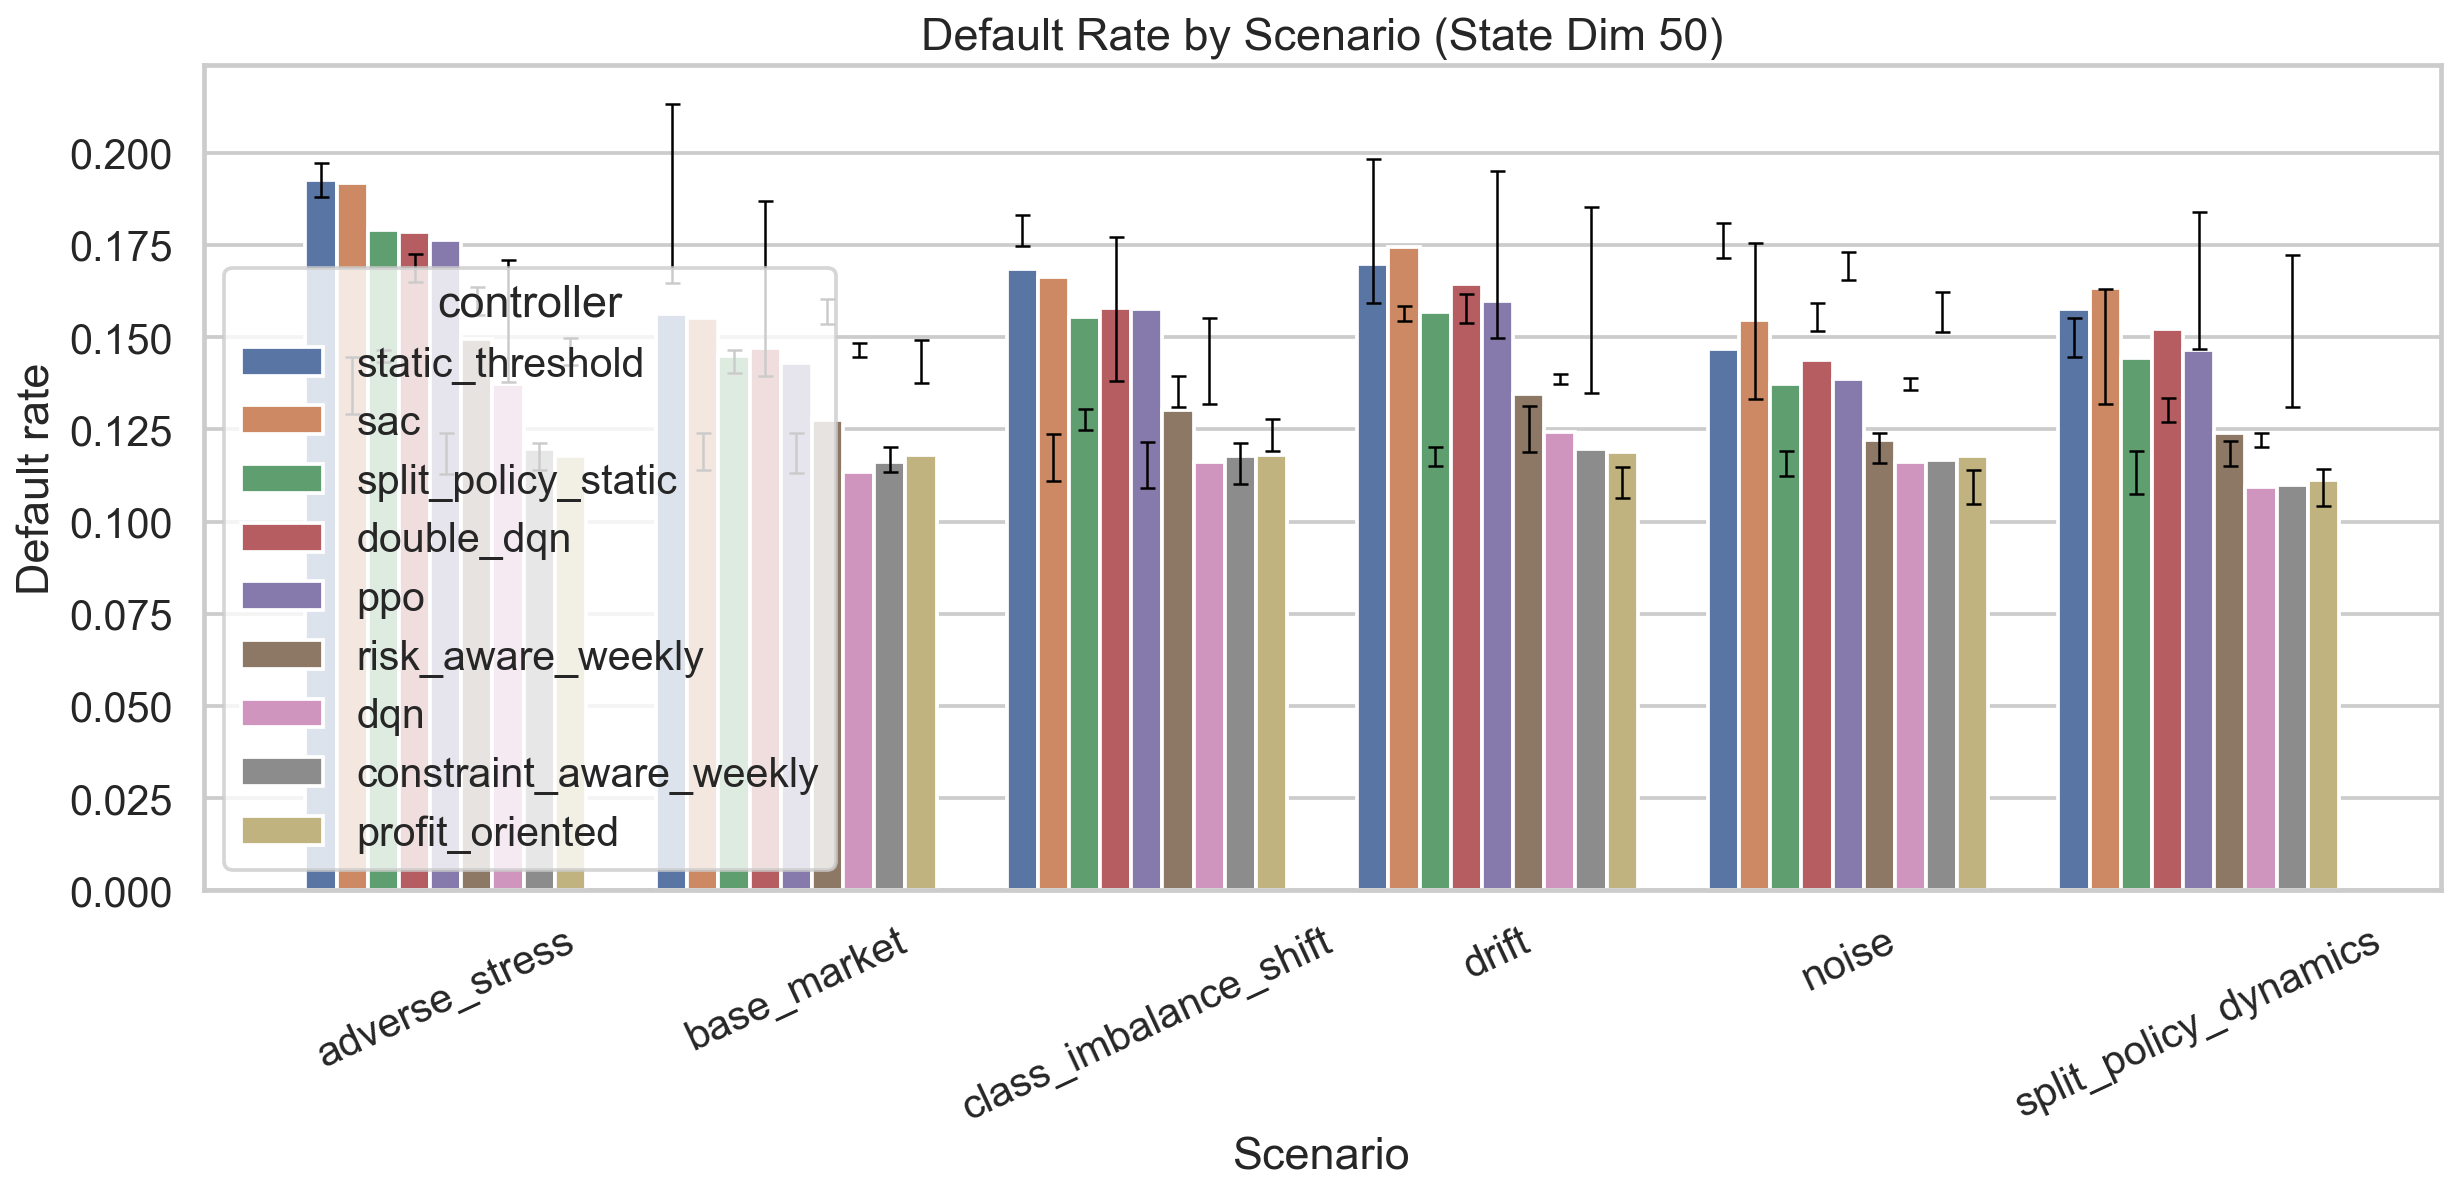
\includegraphics[width=\textwidth]{dim_50/default_rate_by_scenario_dim50.png}
        \caption{50D default-rate comparison}
    \end{subfigure}
    \caption{Rich-state scenario view of profit and default trade-offs.}
    \label{fig:en-scenario-bars-b}
\end{figure}

\begin{figure}[H]
    \centering
    \begin{subfigure}[b]{0.48\textwidth}
        \centering
        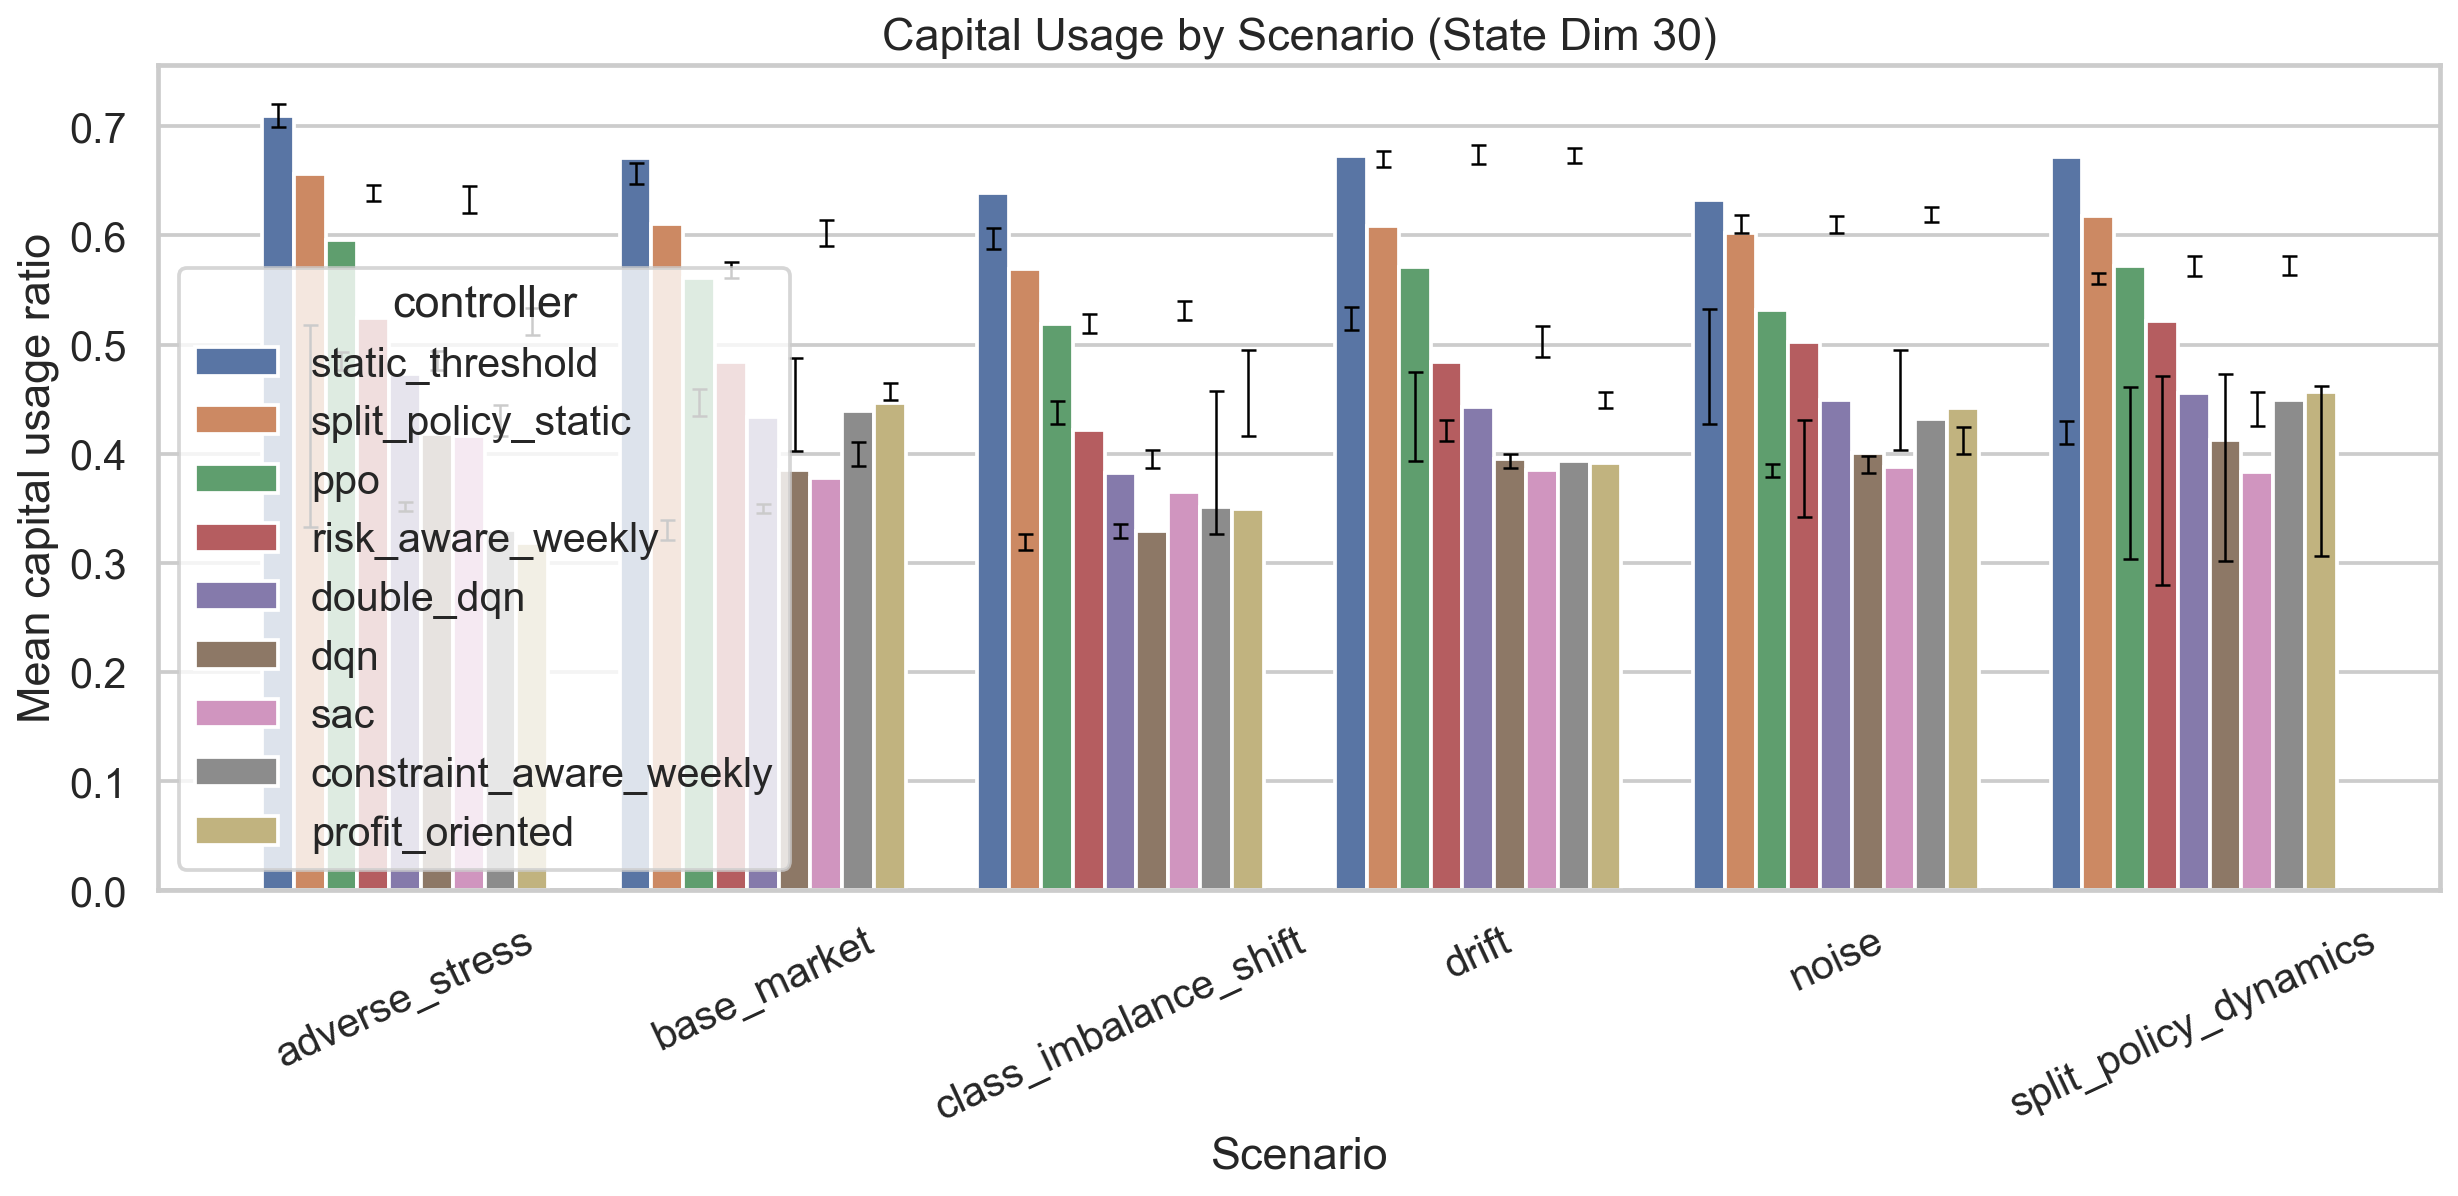
\includegraphics[width=\textwidth]{dim_30/capital_usage_by_scenario_dim30.png}
        \caption{30D capital usage}
    \end{subfigure}
    \hfill
    \begin{subfigure}[b]{0.48\textwidth}
        \centering
        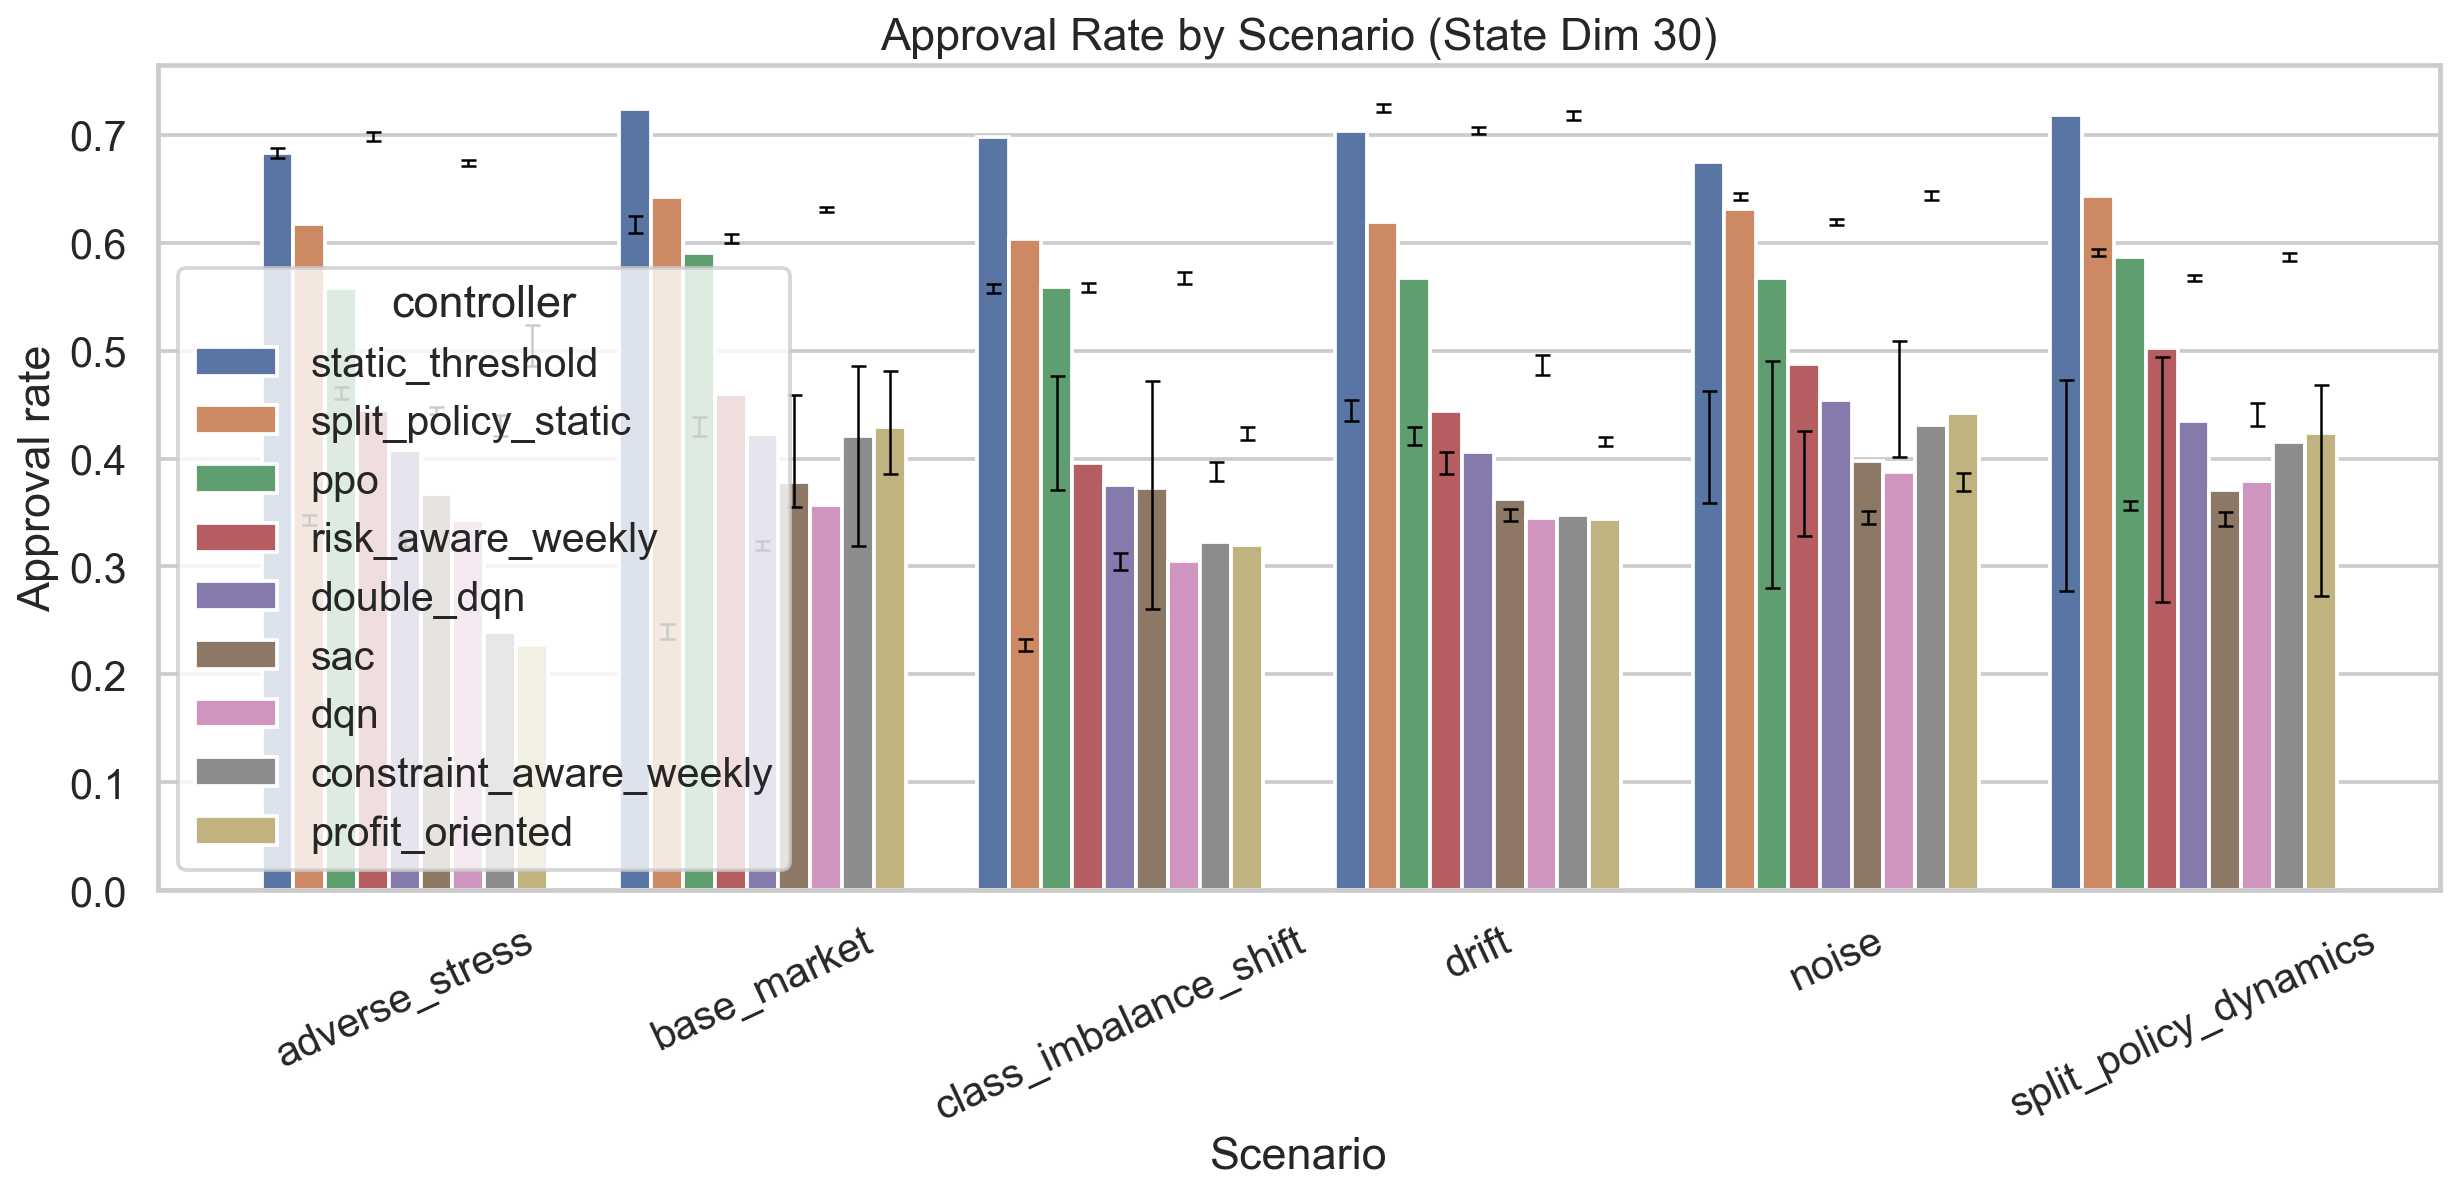
\includegraphics[width=\textwidth]{dim_30/approval_rate_by_scenario_dim30.png}
        \caption{30D approval rate}
    \end{subfigure}
    \caption{Portfolio-allocation trade-offs for the 30D run.}
    \label{fig:en-cap-approval}
\end{figure}

Taken together, Figures \ref{fig:en-scenario-bars-a}--\ref{fig:en-cap-approval} show why the 30D and 50D results are best understood through scenario structure rather than through one scalar curve only. The richest state does help in several places, especially \texttt{base\_market}, \texttt{class\_imbalance\_shift}, and \texttt{split\_policy\_dynamics}, but it does not remove the RL deficit under \texttt{adverse\_stress} and does not overturn the dominance of conservative rule-based search in \texttt{drift}.

\section{Discussion}

\subsection{Why 30D is the most balanced state size}

Something unexpected happens between 20D and 30D. The best RL controller does not just earn more reward---it does so while approving \emph{fewer} loans and using \emph{less} capital. That combination is unusual enough to deserve a closer look at what the 30D additions actually provide.

Read against the manifest, the difference between the two state sizes is precisely the historical memory layer: lagged approval, lagged realized default, lagged realized profit, lagged capital usage, rolling means, rolling profit variability, and lagged threshold changes. Those variables tell the controller whether the latest week is exceptional or part of an emerging pattern. The 30D row in the best-RL table is therefore not a generic ``more is better'' result. It says, specifically, that lagged and rolling memory of \emph{this} portfolio's recent past is the information that lets the agent be more selective and earn more reward at the same time. Drift, noise, and composition-shift environments are where that recent-past signal pays off most directly.

\subsection{Why 50D saturates}

The 50D state size is the natural place to expect the best results, and that is not what the table shows. The added coordinates are not redundant in any obvious sense---they cover segment-level means, rolling reward moments, cumulative totals to date, and threshold-gap history---and yet the best RL reward stops improving. The shape of the curve is the familiar saturation frontier: once the controller already knows current performance, recent history, and lagged threshold behaviour, additional segmentation and stability descriptors do not produce a comparable gain in decision quality at the current training budget.

A second, less comfortable reading sits underneath the saturation story. The 50D run is not merely ``no better.'' It actively harms some algorithms. Double-DQN falls from a positive reward of $69{,}812.02$ at 20D to $-79{,}329.16$ at 50D, and SAC deteriorates sharply as well. The 50D state is therefore both richer and more optimization-demanding. The state itself is not bad. Its control value is conditional on the learning algorithm and the training budget.

\subsection{Why the best baseline still wins overall}

Why does a hand-crafted weekly grid search keep beating six neural-network agents? The answer is uncomfortable but plausible: \texttt{profit\_oriented} and \texttt{constraint\_aware\_weekly} have a structural advantage that has nothing to do with cleverness. They search the same discrete threshold grid the environment exposes, and they evaluate each candidate using the simulator's own weekly economics. There is no value function to fit, no policy to parameterize, and no replay buffer to populate---only the current week, the threshold grid, and the constraint check.

Under the quick profile, RL has only 12 training episodes per seed. That is deliberately small, and it is part of the design rather than a flaw. The fair reading of the leaderboard is not that RL failed. It is that strong hand-crafted policy search remains extremely competitive in a well-structured simulator, and that RL becomes meaningfully better when the state is informative enough and the scenario is favourable enough.

\subsection{Portfolio-quality trade-offs}

The dimensionality experiment is most interesting where several metrics move in opposite directions. The best RL controller at 20D increases approval rate and capital usage relative to 12D, but also slightly worsens default rate. The 30D controller reverses that pattern: it becomes more selective, uses less capital, and improves reward strongly. The 50D controller then relaxes again, with higher approval and capital usage but nearly flat reward.

This sequence is exactly the kind of portfolio trade-off that a thesis should emphasize. Better results do not always mean ``approve more'' or ``reduce default'' in isolation. What matters is the joint movement of profit, default, capital usage, and stability. The 30D result is strong because the joint movement is favorable. The 50D result is weaker because the additional approval and capital consumption do not translate into additional reward.

\subsection{What the current results do and do not establish}

The current evidence establishes several limited but useful findings.
\begin{itemize}[leftmargin=*]
    \item State design matters materially for RL quality.
    \item The marginal value of additional state information is non-linear.
    \item Richer state can improve profitability while preserving or even improving risk metrics in some scenarios.
    \item The benefit of richer state is algorithm-dependent.
\end{itemize}

It does \emph{not} establish that 50D is universally too large, that 30D would remain optimal under a much larger training budget, or that RL is incapable of learning genuinely dynamic weekly policies. Those stronger claims would require a longer-horizon training study, not only the current quick-profile outputs.

\section{Limitations}

Several limitations should be stated directly.
\begin{itemize}[leftmargin=*]
    \item The simulator is synthetic. Its segment parameters and scenarios are economically plausible, but they are not calibrated to confidential production portfolios.
    \item The quick profile is intentionally small. Twelve training episodes per seed are sufficient for an end-to-end controlled experiment, not for a final convergence claim.
    \item The reward is a designed objective, not a discovered one. The relative ranking of controllers is therefore partly a function of the chosen trade-off between profitability, approval pressure, capital usage, and volatility.
    \item The exported confidence intervals quantify uncertainty inside the simulation generator. They do not, by themselves, establish external validity on real bank data.
    \item The best RL policies in this profile are episode-static threshold pairs. Therefore, the current evidence for adaptive weekly threshold movement is weaker than the evidence for better episode-level threshold selection.
\end{itemize}

These limitations do not weaken the core methodological contribution. They simply define the correct boundary of the claim.

\section{Research Contribution}

The contribution of the study lies less in inventing a brand-new RL algorithm and more in combining several research ingredients in one controlled experimental design.
\begin{itemize}[leftmargin=*]
    \item \textbf{Methodological contribution:} credit-scoring control is formulated as weekly portfolio threshold management rather than one-shot application classification.
    \item \textbf{Simulation contribution:} delayed outcomes, late recovery, realized NPV, capital usage, and terminal settlement are made explicit parts of the environment.
    \item \textbf{Experimental contribution:} new and repeat applicants are controlled through separate thresholds, and state representation is varied through a controlled 12D--20D--30D--50D experiment.
    \item \textbf{Benchmarking contribution:} learned policies are evaluated against a diverse and economically interpretable baseline set rather than against a weak static comparator only.
    \item \textbf{Empirical contribution:} the results identify where RL works, where it is limited, and why scenario-level robustness is more informative than a single average score.
\end{itemize}

This is why the thesis contribution should be described as a contribution in \emph{problem formulation, simulation design, experimental methodology, and robustness interpretation}, not only as a leaderboard comparison.

\section{Conclusion}

The goal of this thesis was to evaluate the robustness of a reinforcement learning framework for credit-scoring threshold optimization under different state representations, market scenarios, and portfolio constraints. The research question asked under which conditions reinforcement learning provides a robust improvement over rule-based threshold policies in a delayed-outcome credit-scoring environment.

The thesis achieved this goal by developing the original threshold-control idea into a richer experimental framework. The implemented environment models weekly split thresholds for new and repeat customers, delayed repayments and defaults, late recoveries, realized profit and NPV, capital usage, reward penalties, and terminal settlement. The evaluation covers four state representations, six market scenarios, four RL algorithms, and five rule-based or static baselines. Statistical evidence was added where run-level data allowed paired comparisons.

The first hypothesis, concerning state representation, receives only partial support. The paired reward comparison between 30D and 12D DQN is not statistically significant ($p = 0.41$), meaning the additional state information does not reliably improve the best RL frontier within the full training budget. However, 30D is significantly better than 50D ($p \approx 0$), confirming that the 50D segmentation layer introduces diminishing returns. The 30D state therefore remains the most balanced representation in the sense that it avoids the degradation observed at 50D, even if it does not clearly surpass 12D.

The second hypothesis is strongly confirmed. Across all four dimensions, RL controllers win zero of six scenarios by cumulative reward, zero by expected profit, and zero by lowest default rate. The best overall controller is \texttt{constraint\_aware\_weekly} (profit $3{,}802{,}547$, reward $3{,}666{,}052$), essentially tied with \texttt{profit\_oriented}. RL controllers are not irrelevant: several produce lower default rates than the baselines in specific scenarios, and Double-DQN is the strongest RL agent across all dimensions. But the evidence against universal RL superiority is unambiguous.

The third hypothesis is rejected for the full-profile setting. In the full-profile adverse-stress run, 30D DQN is significantly worse than \texttt{static\_threshold} at the final horizon ($-41{,}507$ profit, $p = 2.8 \times 10^{-7}$). The ``locally worse, globally better'' pattern observed in the quick profile does not generalise to the full training protocol. Full-horizon evaluation with terminal settlement remains methodologically important, but in this experiment it reveals that the static baseline is persistently stronger than the DQN policy under adverse stress.

Overall, the main answer to the research question is conditional. Reinforcement learning can be useful for dynamic credit-scoring threshold optimization when the state representation contains enough portfolio history and when the market scenario contains exploitable structure. However, strong rule-based baselines remain difficult to beat, especially under stress and drift, and more features do not necessarily lead to better policies. The project should therefore be interpreted as a robustness evaluation of RL-based threshold control, not as a claim of unconditional RL superiority.

The main limitations remain the synthetic nature of the simulator, the short quick-profile training budget, the designed reward function, and the episode-static behavior of the best RL policies in the current runs. Future work should test longer training profiles, reward-sensitivity analysis, stronger adaptive RL policies, calibration on real or semi-synthetic credit data, and more explicit regulatory or capital constraints.

\subsection*{A personal observation}

Looking back at the experimental design, the result I found most counterintuitive was that the best RL policies in the quick profile turned out to be episode-static. The whole point of formulating the problem as sequential weekly control was to let an agent respond to changing portfolio conditions, and the agent's reaction in the strongest runs was to pick one threshold pair at the start of the episode and hold it there. I had expected the dimensionality gradient to show up as richer within-episode behaviour. It showed up instead as better episode-level selection. The second surprise was the direction of the adverse-stress result: I had assumed that more state would, eventually, let RL ride out a shock. In the full-profile run it did the opposite---the static baseline pulled further ahead, not closer. Both observations made me more careful about reading dimensionality experiments as if richer state were automatically a step toward more adaptive policy, and they are the part of this thesis I would most like to follow up on with longer training and reward-shaping experiments.

\section*{Statement on the Use of AI Tools}

During the preparation of this thesis, large language model assistants (Claude by Anthropic and ChatGPT by OpenAI) were used as auxiliary tools to support literature search, grammar checking of selected passages, and explanation of mathematical and algorithmic concepts. All experimental design, simulator implementation, data analysis, interpretation of results, and academic responsibility remain entirely with the author.

\bibliographystyle{plain}
\bibliography{references}

\end{document}
